% Rapport — Mini-projet 1 : dimensionnement et planification d'un réseau LTE à Zaghouan
% Compilation : latexmk -pdf rapport.tex
\documentclass[11pt,a4paper,oneside,openany]{report}

% ---------- langue, polices ----------
\usepackage[T1]{fontenc}
\usepackage[utf8]{inputenc}
\usepackage[french]{babel}
\addto\captionsfrench{\renewcommand{\tablename}{Tableau}}
\usepackage{lmodern}
\usepackage{pdfpages}
\usepackage{textcomp}
\DeclareUnicodeCharacter{00D7}{\ensuremath{\times}}
\DeclareUnicodeCharacter{2248}{\ensuremath{\approx}}
\DeclareUnicodeCharacter{00B7}{\ensuremath{\cdot}}
\DeclareUnicodeCharacter{00B1}{\ensuremath{\pm}}
\usepackage{microtype}
\usepackage{csquotes}

% ---------- mise en page ----------
\usepackage[a4paper,left=26mm,right=26mm,top=26mm,bottom=28mm,headsep=9mm,headheight=14pt,footskip=12mm]{geometry}
\usepackage{xcolor}
\definecolor{foret}{HTML}{2E5B3C}
\definecolor{foret2}{HTML}{4F7A45}
\definecolor{mousse}{HTML}{DFE7CB}
\definecolor{eau}{HTML}{1F6485}
\definecolor{terre}{HTML}{B8431F}
\definecolor{or}{HTML}{C4922A}
\definecolor{encre}{HTML}{15211A}
\definecolor{gris}{HTML}{56634F}
\definecolor{papier}{HTML}{F4F5EC}
\linespread{1.08}
\setlength{\parskip}{0.45em}
\setlength{\parindent}{0pt}

\usepackage{graphicx}
\graphicspath{{figures/}{../04-atoll/exports/}{../04-atoll/captures/}{../02-dimensionnement/figures/}{../05-presentation/deck/assets/atoll/}}
\usepackage{booktabs,tabularx,multirow,array,colortbl,longtable}
\usepackage[font=small,labelfont=bf,labelsep=period,format=plain,justification=justified,singlelinecheck=true]{caption}
\usepackage{subcaption}
\usepackage{float}
\usepackage{enumitem}
\setlist{itemsep=0.15em,topsep=0.3em}
\usepackage[locale=FR,per-mode=symbol,group-minimum-digits=4]{siunitx}
\sisetup{range-phrase={ à },list-final-separator={ et }}
\DeclareSIUnit\dBm{dBm}
\DeclareSIUnit\dBi{dBi}
\DeclareSIUnit\kbps{kbps}
\DeclareSIUnit\Mbps{Mbps}
\usepackage{amsmath}
\usepackage{tikz}
\usetikzlibrary{positioning,arrows.meta,shapes.geometric,calc,fit,backgrounds}
\usepackage[most]{tcolorbox}

% ---------- titres ----------
\usepackage{titlesec}
\titleformat{\chapter}[display]
  {\normalfont\bfseries}
  {\large\chaptertitlename\ \thechapter}
  {0.8em}
  {\huge}[\vspace{0.3em}\titlerule]
\titleformat{name=\chapter,numberless}[display]
  {\normalfont\bfseries}{}{0pt}{\huge}[\vspace{0.3em}\titlerule]
\titlespacing*{\chapter}{0pt}{-12pt}{24pt}
\titleformat{\section}{\normalfont\Large\bfseries}{\thesection}{0.8em}{}
\titleformat{\subsection}{\normalfont\large\bfseries}{\thesubsection}{0.7em}{}
\titleformat{\subsubsection}{\normalfont\normalsize\bfseries}{}{0em}{}
\titlespacing*{\section}{0pt}{1.4em}{0.5em}
\titlespacing*{\subsection}{0pt}{1.1em}{0.35em}

% ---------- en-têtes ----------
\usepackage{fancyhdr}
\pagestyle{fancy}
\fancyhf{}
\renewcommand{\chaptermark}[1]{\markboth{#1}{}}
\renewcommand{\sectionmark}[1]{\markright{\thesection\ #1}}
\fancyhead[L]{\small\itshape\leftmark}
\fancyhead[R]{\small\itshape\rightmark}
\fancyfoot[C]{\thepage}
\renewcommand{\headrulewidth}{0.4pt}
\fancypagestyle{plain}{\fancyhf{}\fancyfoot[C]{\thepage}\renewcommand{\headrulewidth}{0pt}}

% ---------- encadrés ----------
\newtcolorbox{retenir}[1][Synthèse]{enhanced,breakable,colback=mousse!45,colframe=foret,boxrule=0pt,leftrule=3pt,arc=2pt,
  left=10pt,right=10pt,top=6pt,bottom=6pt,fonttitle=\bfseries\small,coltitle=foret,colbacktitle=mousse!45,
  title={#1},attach title to upper={\par\smallskip},before skip=10pt,after skip=10pt}
\newtcolorbox{verdict}[1][Verdict]{enhanced,breakable,colback=or!10,colframe=or,boxrule=0pt,leftrule=3pt,arc=2pt,
  left=10pt,right=10pt,top=6pt,bottom=6pt,fonttitle=\bfseries\small,coltitle=or!70!black,colbacktitle=or!10,
  title={#1},attach title to upper={\par\smallskip},before skip=10pt,after skip=10pt}

\newtcolorbox{cours}[1]{enhanced,breakable,colback=white,colframe=eau,boxrule=0.5pt,arc=1.5pt,
  left=9pt,right=9pt,top=5pt,bottom=5pt,fonttitle=\bfseries\small,coltitle=white,colbacktitle=eau,
  title={Rappel du cours : #1},segmentation style={dashed,eau!50,line width=0.4pt},
  before skip=10pt,after skip=10pt}
\newcommand{\application}{\tcblower\textbf{Dans notre projet.}\ }

% ---------- tableaux ----------
\newcolumntype{L}{>{\raggedright\arraybackslash}X}
\newcolumntype{C}{>{\centering\arraybackslash}X}
\renewcommand{\arraystretch}{1.18}
\newcommand{\ok}{{\color{foret}\textbf{atteint}}}
\newcommand{\ko}{{\color{terre}\textbf{non atteint}}}
\newcommand{\gardee}{{\color{foret}\textbf{gardée}}}
\newcommand{\rejetee}{{\color{terre}\textbf{rejetée}}}
\newcommand{\thead}[1]{\bfseries\begin{tabular}[b]{@{}c@{}}#1\end{tabular}}

% ---------- bibliographie, liens ----------
\usepackage[numbers,sort&compress]{natbib}
\bibliographystyle{abbrvnat}
\usepackage[hidelinks,pdfusetitle]{hyperref}
\hypersetup{pdftitle={Réseau LTE Zaghouan — rapport du mini-projet 1},pdfauthor={Youssef Hamdani, Rayen Hamza},pdfsubject={Planification et optimisation des réseaux, RT5, INSAT}}
\usepackage[nameinlink,noabbrev]{cleveref}
\crefname{figure}{figure}{figures}\crefname{table}{tableau}{tableaux}\crefname{chapter}{chapitre}{chapitres}
\newcommand{\crefpairconjunction}{ et }\newcommand{\crefmiddleconjunction}{, }\newcommand{\creflastconjunction}{ et }\newcommand{\crefrangeconjunction}{ à }
\crefname{section}{section}{sections}\crefname{equation}{équation}{équations}\crefname{appendix}{annexe}{annexes}

\begin{document}

% =====================================================================  PAGE DE GARDE

\includepdf[pages=1]{page-de-garde.pdf}
\setcounter{page}{1}

\pagenumbering{roman}
\chapter*{Résumé}
\addcontentsline{toc}{chapter}{Résumé}

Ce rapport présente le dimensionnement, la planification et l'optimisation d'un réseau LTE (bande~3, \SI{1800}{\mega\hertz}, porteuse de \SI{20}{\mega\hertz}) sur une zone réelle de \num{10} × \SI{10}{\kilo\metre} autour de Zaghouan (Tunisie), qui réunit un centre urbain dense, une campagne et le massif du Djebel Zaghouan. Dans une première étape, un dimensionnement analytique fixe les marges (effet de masque log-normal, pénétration, interférence), établit le bilan de liaison avec le modèle COST-231 Hata et en déduit le rayon des cellules : \SI{0,64}{\kilo\metre} en ville (indoor) et \SI{2,06}{\kilo\metre} en campagne (outdoor), la liaison montante étant limitante. La couverture impose 21 sites tri-sectoriels, alors que la capacité n'en demanderait que 5 dans le centre ; la réutilisation de fréquences retenue est $K = 1$.

Dans une seconde étape, ce réseau est construit dans Atoll 3.3 sur des cartes réelles (relief Copernicus, occupation du sol ESA WorldCover, population WorldPop) avec le modèle Cost-Hata et la diffraction sur le relief. Les prédictions de niveau de signal, de serveur, de recouvrement, de C/(I+N) et de débit, puis des simulations Monte-Carlo à 10, 100 et \num{1000} utilisateurs, montrent un réseau couvert en ville (\SI{99,5}{\percent} en indoor) mais troué derrière le massif (\SI{83,4}{\percent} de la campagne en outdoor), et dont les rejets d'utilisateurs viennent du signal et non de la capacité. Huit actions d'optimisation, mesurées une à une (tilt, retrait d'un site, deux nouveaux sites, ACP, ANR), portent la couverture rurale à \SI{94,3}{\percent} de la surface (\SI{97,9}{\percent} de la population) et la couverture urbaine à \SI{99,7}{\percent}, avec 21 sites, le nombre prévu par le calcul. Sur les mêmes \num{1041} utilisateurs simulés, les rejets passent de 108 à 71. Le calcul analytique a donc donné le bon nombre de sites, et la simulation sur le relief réel leurs bons emplacements.

\medskip
\textbf{Mots-clés :} LTE, planification radio, bilan de liaison, COST-231 Hata, Atoll, Monte-Carlo, DCFI, optimisation, ACP.

\vspace{2em}
\section*{Abstract}

This report covers the dimensioning, planning and optimisation of an LTE network (band~3, 1800~MHz, 20~MHz carrier) over a real 10 × 10~km area around Zaghouan, Tunisia. An analytical link budget with the COST-231 Hata model gives uplink-limited cell radii of 0.64~km (urban, indoor) and 2.06~km (rural, outdoor), hence 21 tri-sector sites with frequency reuse 1. The network is then built in Atoll 3.3 on real terrain, land-cover and population data. Coverage, interference and throughput predictions, followed by Monte-Carlo simulations with 10, 100 and 1000 users, show that the remaining problem is coverage behind the mountain, not capacity. Eight measured optimisation actions raise rural outdoor coverage from 83.4\,\% to 94.3\,\% while keeping 21 sites, the number predicted by the analytical step.

\cleardoublepage
{\hypersetup{linkcolor=encre}\tableofcontents}
\cleardoublepage
\listoffigures
\listoftables
\cleardoublepage
\pagenumbering{arabic}

\chapter{Introduction}
\label{ch-intro}

\section{Contexte}

Un opérateur souhaite déployer un réseau 4G sur la ville de Zaghouan et sa campagne. Le sujet du mini-projet~\cite{afif2026sujet} nous place dans le rôle de l'ingénieur planification radio chargé de l'étude : établir le cahier des charges de l'interface radio, dimensionner le réseau, le construire et le vérifier dans l'outil de planification Atoll~\cite{atoll33}, l'optimiser, puis présenter le résultat à la direction.

La zone d'étude est un carré de \num{10} × \SI{10}{\kilo\metre} (\SI{100}{\kilo\metre\squared}) qui contient trois milieux très différents : le centre urbain de Zaghouan, une campagne de prairies et de cultures parsemée de villages, et le Djebel Zaghouan, un massif boisé qui culmine à \SI{1238}{\metre} sur notre modèle de terrain. Nous avons choisi cette zone pour traiter les deux parties du dimensionnement demandées par le sujet, par la capacité en ville et par la couverture en campagne. Le relief y crée en plus des zones d'ombre radio, qui donnent matière à l'optimisation.

\section{Objectifs}

Le travail suit les deux étapes du sujet :
\begin{enumerate}
  \item \textbf{Étape 1, dimensionnement analytique :} norme, environnement, objectifs de couverture et de trafic ; bilan de liaison, rayon de cellule, nombre et position des sites ; capacité, motif de réutilisation et plan de fréquences.
  \item \textbf{Étape 2, planification avec Atoll :} import du terrain, construction du réseau issu de l'Étape 1, prédictions de couverture et de débit, simulations Monte-Carlo pour 10, 100 et \num{1000} utilisateurs, comparaison aux objectifs, optimisation itérative.
\end{enumerate}
Le rapport se termine par une comparaison critique entre les résultats des deux étapes et par les limites de l'étude.

\section{Démarche}

La zone, la bande, le modèle de propagation et les hypothèses de trafic sont les mêmes dans l'Étape 1 et dans Atoll, ce qui permet de comparer les deux étapes à la fin. Toutes les valeurs d'entrée sont rassemblées dans un tableau d'hypothèses unique (\cref{ch-cdc}), repris par notre script de calcul et par la configuration d'Atoll. Pendant l'optimisation, chaque action est appliquée seule, mesurée avec le même script sur les rasters exportés d'Atoll, puis gardée ou annulée.

\begin{figure}[H]
\centering
\begin{tikzpicture}[
  node distance=5mm and 2mm,
  box/.style={draw=foret,fill=mousse!50,rounded corners=2pt,align=center,font=\scriptsize,text width=26mm,minimum height=13mm,inner sep=3pt},
  arr/.style={-{Stealth[length=2.2mm]},foret,thick}]
  \node[box] (a) {\textbf{Cahier des charges}\\zone, norme,\\objectifs};
  \node[box,right=of a] (b) {\textbf{Dimensionnement}\\bilan de liaison,\\$R$, sites, $K$};
  \node[box,right=of b] (c) {\textbf{Atoll}\\cartes réelles,\\20 sites};
  \node[box,right=of c] (d) {\textbf{Prédictions}\\signal, C/(I+N),\\débits};
  \node[box,right=of d] (e) {\textbf{Monte-Carlo}\\10, 100, 1\,000\\utilisateurs};
  \node[box,below=10mm of e,fill=or!15,draw=or] (f) {\textbf{Optimisation}\\une action\\à la fois};
  \node[box,fill=white] (g) at (b |- f) {\textbf{Bilan}\\Étape 1 contre\\Étape 2};
  \draw[arr] (a)--(b); \draw[arr] (b)--(c); \draw[arr] (c)--(d); \draw[arr] (d)--(e); \draw[arr] (e)--(f); \draw[arr] (f)--(g);
  \draw[arr,or!80!black] (f.north west) to[bend left=25] node[pos=0.55,left,font=\tiny,text=gris,align=right]{chaque action\\est re-mesurée} (d.south);
\end{tikzpicture}
\caption{Démarche du projet.}
\label{fig-demarche}
\end{figure}

\section{Outils et données}

\begin{itemize}
  \item \textbf{Atoll 3.3} (Forsk), module LTE~\cite{atoll33}, installé dans une machine virtuelle Windows.
  \item \textbf{Données géographiques ouvertes :} relief Copernicus DEM GLO-30~\cite{copernicusdem}, occupation du sol ESA WorldCover 2021~\cite{worldcover2022}, population WorldPop 2020~\cite{worldpop2018}.
  \item \textbf{Données de marché :} tableau de bord trimestriel de l'Instance Nationale des Télécommunications~\cite{intt2025tr4}.
  \item \textbf{Scripts Python} (calcul de l'Étape 1, préparation des cartes, mesure de la couverture par zone sur les rasters d'Atoll, tracé des DCFI) ; ils sont fournis avec le projet.
\end{itemize}

\section{Organisation du rapport}

Le \cref{ch-cdc} présente le cahier des charges. Le \cref{ch-dim} détaille le dimensionnement analytique. Le \cref{ch-atoll} décrit la construction du réseau dans Atoll, le \cref{ch-pred} les prédictions et le \cref{ch-mc} les simulations Monte-Carlo. Le \cref{ch-opt} présente la démarche d'optimisation, action par action. Le \cref{ch-disc} compare les deux étapes et discute les limites, avant la conclusion.

\chapter{Cahier des charges}
\label{ch-cdc}

Ce chapitre fixe le cadre de l'étude : zone, norme et bande, équipements, objectifs et modèle de trafic. Chaque valeur est sourcée ; celles qui relèvent de notre jugement sont signalées comme hypothèses.

\section{La zone d'étude}
\label{sec-zone}

La zone couvre \num{10} × \SI{10}{\kilo\metre} en projection UTM 32N (EPSG:32632), de X = \SIrange{596}{606}{\kilo\metre} et Y = \SIrange{4022}{4032}{\kilo\metre}. Elle compte \num{25359} habitants d'après WorldPop 2020~\cite{worldpop2018}. L'occupation du sol, mesurée sur ESA WorldCover~\cite{worldcover2022}, se répartit en prairies (\SI{38,0}{\percent}), forêt (\SI{27,5}{\percent}), arbustes (\SI{13,3}{\percent}), cultures (\SI{13,0}{\percent}), bâti (\SI{6,6}{\percent}), sol nu (\SI{1,3}{\percent}) et eau (\SI{0,1}{\percent}).

Nous l'avons découpée en trois zones à partir des cartes (\cref{fig-zone,tab-zones}) :
\begin{itemize}
  \item le \textbf{centre urbain}, défini comme l'ensemble des pixels de \SI{100}{\metre} dont la densité atteint \SI{1000}{hab\per\kilo\metre\squared} ;
  \item le \textbf{massif}, au-dessus de \SI{600}{\metre} d'altitude : il correspond au parc national du Djebel Zaghouan, presque inhabité, où aucun site n'est autorisé et où nous ne fixons pas d'objectif ;
  \item la \textbf{zone rurale}, qui forme le reste.
\end{itemize}

\begin{figure}[H]
\centering
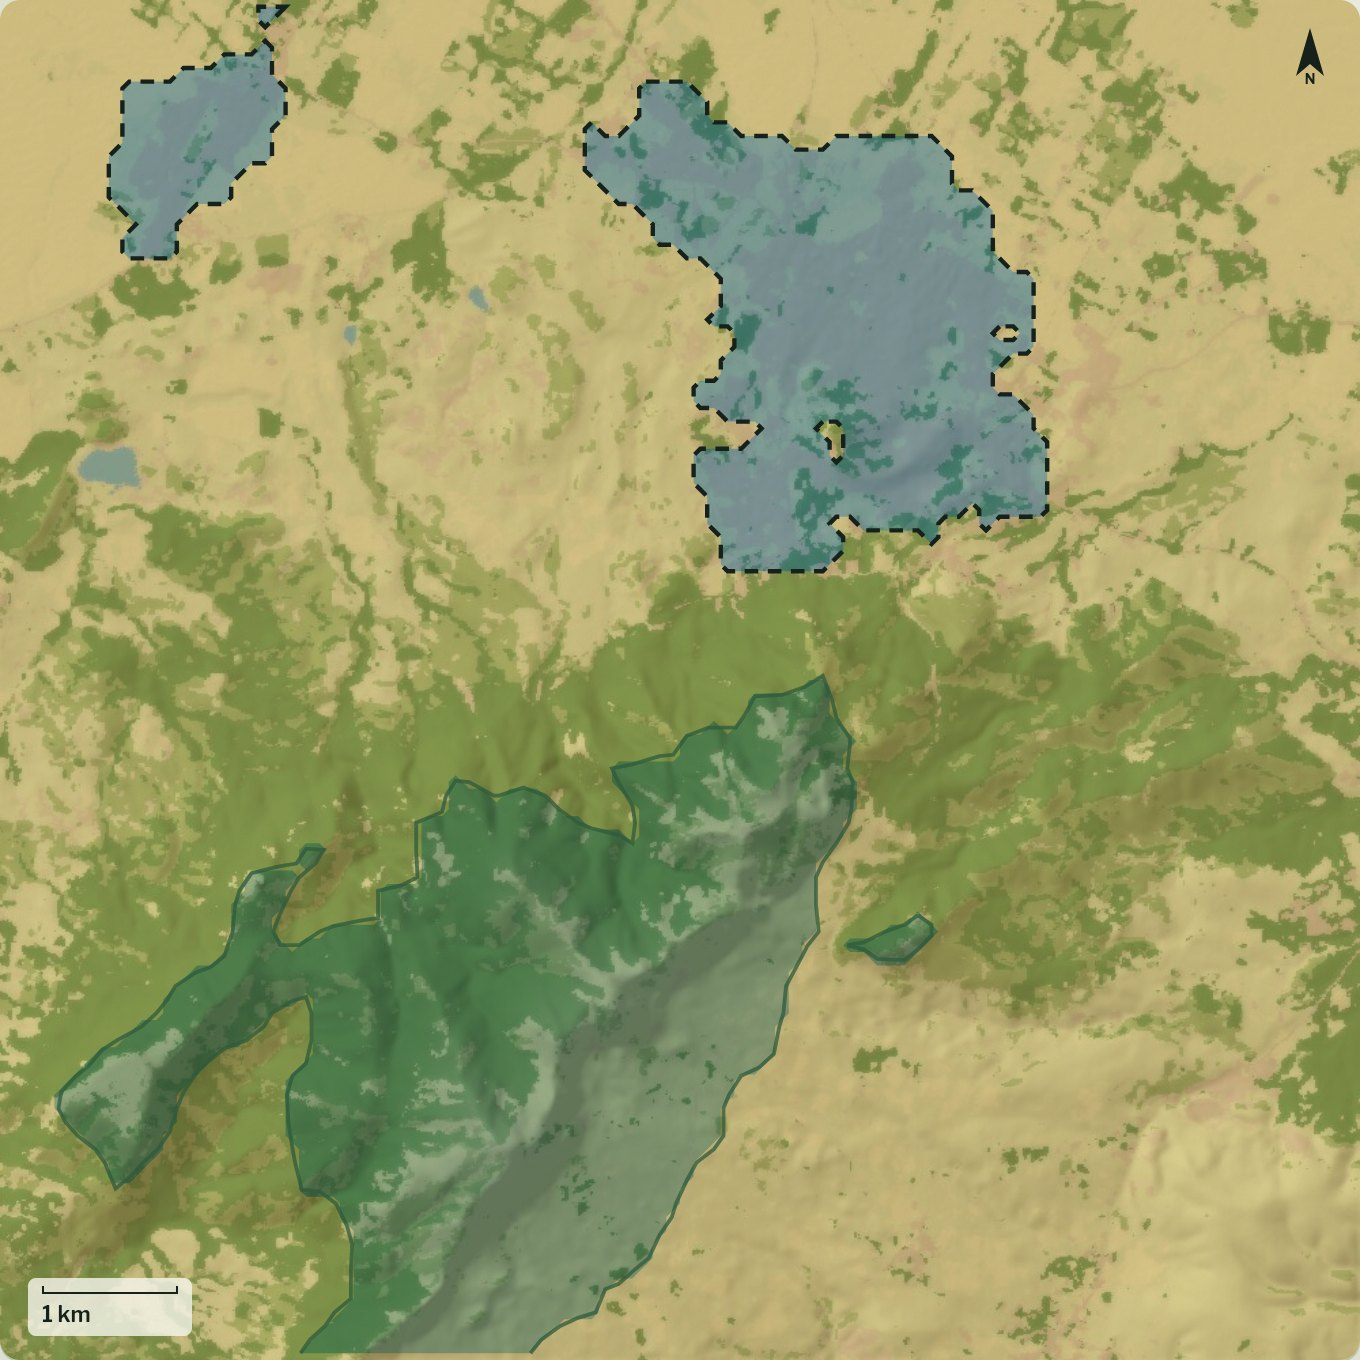
\includegraphics[width=0.62\textwidth]{zone.jpg}
\caption{Zone d'étude et découpage en trois zones.}
\label{fig-zone}
\end{figure}

La \cref{fig-zone} superpose l'occupation du sol (ESA WorldCover) au relief ombré (Copernicus). Le centre urbain est tracé en bleu, le massif au-dessus de \SI{600}{\metre} en vert foncé.

\begin{table}[H]
\centering
\caption{Les trois zones de l'étude.}
\label{tab-zones}
\begin{tabularx}{\textwidth}{@{}lLrrL@{}}
\toprule
\thead{Zone} & \thead{Définition} & \thead{Surface} & \thead{Habitants} & \thead{Stratégie} \\
\midrule
Centre urbain & densité $\geq$ \SI{1000}{hab\per\kilo\metre\squared} & \SI{8,57}{\kilo\metre\squared} & \num{13590} & capacité, objectif indoor \\
Rural & reste de la zone & \SI{76,95}{\kilo\metre\squared} & \num{11476} & couverture, objectif outdoor \\
Massif & altitude $\geq$ \SI{600}{\metre} & \SI{14,48}{\kilo\metre\squared} & \num{292} & aucun site, aucun objectif \\
\midrule
\textbf{Total} & & \SI{100}{\kilo\metre\squared} & \num{25359} & \\
\bottomrule
\end{tabularx}
\end{table}

\begin{cours}{objectif selon le contexte}
En zone urbaine ou suburbaine, l'objectif est d'assurer une capacité en trafic suffisante pour un grand nombre d'abonnés. En zone rurale, l'objectif est la couverture la plus complète possible, sans besoin de capacité élevée~\cite{afif2026cours}.
\application Le centre urbain est dimensionné par la capacité (§\,3.3 du sujet) et la campagne par la couverture (§\,3.2). Dans chaque zone, nous calculons quand même les deux besoins et gardons le plus grand (\cref{tab-sites-final}).
\end{cours}

\section{Choix de la norme}

\paragraph{LTE plutôt que GSM.} Le sujet demande des cartes de débit en liaison descendante (DL) et montante (UL) ainsi que des simulations Monte-Carlo. Dans Atoll 3.3, ces deux outils existent pour l'UMTS, le WiMAX et le LTE, mais pas pour le GSM. Nous avons retenu le LTE, la mieux documentée des trois~\cite{holma2011,sesia2011}. Le cours et le sujet sont rédigés dans la logique GSM (canaux, Erlang, motif de réutilisation) ; nous traduisons chaque étape en LTE au \cref{ch-dim}. En Tunisie, le LTE porte aussi l'essentiel du trafic : fin 2025, \SI{84}{\percent} des smartphones sont compatibles 4G et \SI{9}{\percent} compatibles 5G~\cite{intt2025tr4}.

\paragraph{Bande 3 (\SI{1800}{\mega\hertz}) plutôt que bande 20 (\SI{800}{\mega\hertz}).} Les deux bandes sont utilisées en Tunisie. La bande~20 ne fait que $2 × \SI{30}{\mega\hertz}$ pour trois opérateurs, soit au plus \SI{10}{\mega\hertz} chacun, alors que la bande~3 ($2 × \SI{75}{\mega\hertz}$) permet une porteuse de \SI{20}{\mega\hertz}~\cite{ts36101}. Le calcul du \cref{sec-800-1800} compare les deux bandes : le \SI{800}{\mega\hertz} porte plus loin et demande moins de sites aujourd'hui, mais sature en capacité quand le trafic augmente.

\begin{table}[H]
\centering
\caption{Norme et spectre retenus.}
\label{tab-norme}
\begin{tabularx}{\textwidth}{@{}lLl@{}}
\toprule
\thead{Paramètre} & \thead{Valeur} & \thead{Source} \\
\midrule
Norme & LTE (E-UTRA) FDD ; OFDMA en DL, SC-FDMA en UL & \cite{ts36211} \\
Bande & bande 3 : UL \SIrange{1710}{1785}{\mega\hertz}, DL \SIrange{1805}{1880}{\mega\hertz} & \cite{ts36101} \\
Porteuse & \SI{20}{\mega\hertz}, 100 blocs de ressources (RB) ; EARFCN 1300 : centre DL \SI{1815}{\mega\hertz}, UL \SI{1720}{\mega\hertz} & Atoll \\
Réutilisation & $K = 1$ : la même porteuse dans toutes les cellules (\cref{sec-reuse}) & calcul \\
\bottomrule
\end{tabularx}
\end{table}

\section{Équipements}

Les paramètres des équipements (\cref{tab-equip}) reprennent les modèles LTE fournis par Atoll, adaptés à notre porteuse de \SI{20}{\mega\hertz}. Les modèles de station d'Atoll sont prévus pour \SI{10}{\mega\hertz} et \SI{43}{\dBm}, ce qui donne une puissance par sous-porteuse du signal de référence (RS EPRE) de $43 - 10\log_{10} 600 = \SI{15,2}{\dBm}$. Pour garder cette puissance par sous-porteuse sur \num{1200} sous-porteuses, il faut $15{,}2 + 10\log_{10} 1200 = \SI{46}{\dBm}$. À puissance constante, doubler la bande ferait perdre \SI{3}{\deci\bel} par sous-porteuse.

\begin{table}[H]
\centering
\caption{Paramètres des équipements.}
\label{tab-equip}
\begin{tabularx}{\textwidth}{@{}lLl@{}}
\toprule
\thead{Paramètre} & \thead{Valeur} & \thead{Source} \\
\midrule
Puissance de l'eNodeB & \SI{46}{\dBm} (\SI{40}{\watt}) sur \SI{20}{\mega\hertz} & Atoll, calcul \\
Facteur de bruit de l'eNodeB & \SI{5}{\deci\bel} & Atoll \\
Antenne & tri-secteur \ang{65}, \SI{18}{\dBi} ; à \SI{30}{\metre} ; tilt électrique \ang{4} (urbain), \ang{2} (rural) ; MIMO 2 × 2 & Atoll \\
Pertes d'émission et de réception & \SI{1}{\deci\bel} (tête radio déportée en haut du mât) & hypothèse \\
Puissance du terminal & \SI{23}{\dBm} (classe de puissance 3) & \cite{ts36101} \\
Facteur de bruit du terminal & \SI{8}{\deci\bel} ; gain d'antenne \SI{0}{\dBi} & Atoll \\
Perte de corps & \SI{3}{\deci\bel} en VoIP, \SI{0}{\deci\bel} en données & Atoll \\
\bottomrule
\end{tabularx}
\end{table}

Le choix d'une tête radio déportée en haut du mât ramène les pertes de câble à environ \SI{1}{\deci\bel}, au lieu d'environ \SI{2,3}{\deci\bel} pour \SI{30}{\metre} de câble coaxial ; un amplificateur de mât devient alors inutile.

\section{Objectifs de couverture et de qualité}
\label{sec-objectifs}

\begin{table}[H]
\centering
\caption{Objectifs du cahier des charges.}
\label{tab-objectifs}
\begin{tabularx}{\textwidth}{@{}lL@{}}
\toprule
\thead{Objectif} & \thead{Valeur} \\
\midrule
Couverture du centre urbain & \SI{95}{\percent} de la surface, \textbf{en indoor} \\
Couverture de la campagne & \SI{95}{\percent} de la surface, \textbf{en outdoor} \\
Massif & aucun objectif \\
Débit en bord de cellule & \SI{1024}{\kbps} en DL, \SI{128}{\kbps} en UL \\
Charge maximale d'une cellule à l'heure chargée & \SI{80}{\percent} \\
\bottomrule
\end{tabularx}
\end{table}

Le débit visé en bord de cellule est celui du service \enquote{High Speed Internet} d'Atoll (\SI{1024}{\kbps} en DL, \SI{128}{\kbps} en UL), ce qui permet de le vérifier directement sur les cartes de débit et dans les simulations. Le bearer le plus robuste accepté par ce service est le bearer~4 (QPSK 1/3), avec un seuil de SINR de \SI{-1}{\deci\bel} dans Atoll : c'est la qualité minimale à garantir en bord de cellule. La charge maximale de \SI{80}{\percent} joue en LTE le rôle du taux de blocage de la loi d'Erlang~B, en gardant une réserve dans chaque cellule.

\section{Modèle de trafic}
\label{sec-trafic}

Les données de marché viennent du tableau de bord de l'INTT pour le quatrième trimestre 2025~\cite{intt2025tr4}.

\begin{table}[H]
\centering
\caption{Hypothèses de trafic.}
\label{tab-trafic}
\begin{tabularx}{\textwidth}{@{}lLl@{}}
\toprule
\thead{Paramètre} & \thead{Valeur} & \thead{Source} \\
\midrule
Pénétration de la data mobile & \SI{93,9}{\percent} par habitant & \cite{intt2025tr4} \\
Part de marché de l'opérateur & \SI{30}{\percent}, part médiane des trois opérateurs (\SI{43,5}{\percent}, \SI{30,4}{\percent}, \SI{25,8}{\percent}) & \cite{intt2025tr4} \\
Terminaux compatibles LTE & \SI{93}{\percent} (\SI{84}{\percent} 4G + \SI{9}{\percent} 5G) & \cite{intt2025tr4} \\
Volume de données & \SI{9,5}{Go} par abonné et par mois (\SI{6,8}{Go} fin 2023) & \cite{intt2025tr4} \\
Part de l'heure chargée & \SI{10}{\percent} du trafic journalier & hypothèse \\
Répartition DL / UL & \SI{90}{\percent} / \SI{10}{\percent} & hypothèse \\
\bottomrule
\end{tabularx}
\end{table}

Le débit moyen d'un abonné à l'heure chargée vaut donc
\begin{equation}
  \frac{\SI{9,5}{Go} × 8}{30~\text{jours}} × \SI{10}{\percent} × \frac{1}{\SI{3600}{\second}} \approx \SI{70,4}{\kbps},
\end{equation}
dont \SI{63,3}{\kbps} en DL et \SI{7,0}{\kbps} en UL. Le volume mensuel a augmenté d'environ \SI{40}{\percent} en deux ans (de 6,8 à \SI{9,5}{Go}) : nous utilisons ce rythme pour vérifier que le réseau tient dans cinq ans.

\chapter{Dimensionnement analytique}
\label{ch-dim}

Ce chapitre correspond à l'Étape 1 du sujet. Tous les résultats sont produits par notre script de calcul à partir du tableau d'hypothèses du \cref{ch-cdc}.

\section{Les marges}
\label{sec-marges}

\subsection{Effet de masque et probabilité de couverture}

Autour de la valeur moyenne donnée par le modèle de propagation, le niveau reçu varie d'un point à l'autre à cause du relief et des bâtiments. Cette variation, l'effet de masque, suit une loi log-normale : en décibels, une loi normale d'écart-type $\sigma$~\cite{rappaport2002}. Nous retenons $\sigma = \SI{8}{\deci\bel}$ en ville et $\sigma = \SI{6}{\deci\bel}$ en campagne, valeurs usuelles pour ces milieux.

L'objectif porte sur \SI{95}{\percent} de la \emph{surface} de la cellule. Le bord est le point le plus défavorable, donc une probabilité plus faible y suffit. La formule de Jakes~\cite{jakes1974} relie les deux probabilités :
\begin{equation}
  F_u = \frac{1}{2}\left[1 - \operatorname{erf}(a) + \exp\!\left(\frac{1 - 2ab}{b^2}\right)\left(1 - \operatorname{erf}\!\left(\frac{1 - ab}{b}\right)\right)\right],
  \qquad a = \frac{-M}{\sigma\sqrt{2}}, \quad b = \frac{10\,n\log_{10} e}{\sigma\sqrt{2}},
  \label{eq-jakes}
\end{equation}
où $F_u$ est la fraction de la surface couverte, $M$ la marge au bord de la cellule et $n$ l'exposant d'affaiblissement. Avec le modèle de Hata (\cref{sec-hata}), la pente vaut $44{,}9 - 6{,}55\log_{10} 30 = \SI{35,2}{\deci\bel}$ par décade, soit $n = 3{,}52$. La résolution de l'équation~\eqref{eq-jakes} pour $F_u = \SI{95}{\percent}$ donne le \cref{tab-jakes}.

\begin{table}[H]
\centering
\caption{Marges d'effet de masque (Jakes, $n = 3{,}52$).}
\label{tab-jakes}
\begin{tabular}{@{}lccccc@{}}
\toprule
\thead{Zone} & \thead{$\sigma$ (dB)} & \thead{$b$} & \thead{$a$} & \thead{Probabilité au bord} & \thead{Marge (dB)} \\
\midrule
Urbain & 8 & 1,352 & $-0{,}767$ & \SI{86,1}{\percent} & \textbf{8,7} \\
Rural & 6 & 1,803 & $-0{,}690$ & \SI{83,5}{\percent} & \textbf{5,9} \\
\bottomrule
\end{tabular}
\end{table}

\begin{figure}[H]
\centering
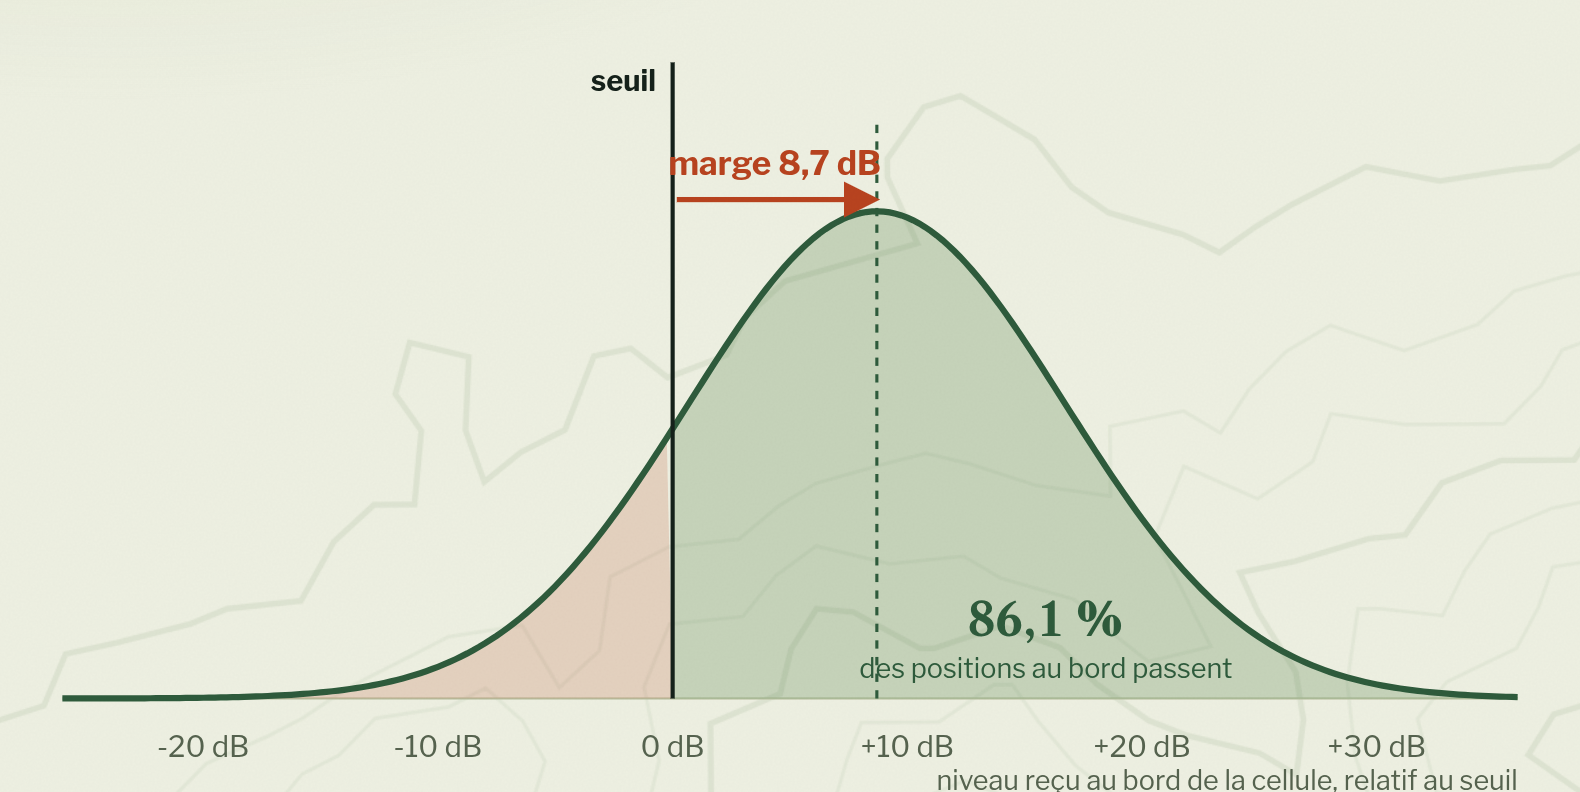
\includegraphics[width=0.72\textwidth]{marges-gauss.png}
\caption{Marge d'effet de masque au bord d'une cellule urbaine.}
\label{fig-gauss}
\end{figure}

La \cref{fig-gauss} montre la distribution du niveau reçu au bord d'une cellule urbaine ($\sigma = \SI{8}{\deci\bel}$). Avec une moyenne \SI{8,7}{\deci\bel} au-dessus du seuil, \SI{86,1}{\percent} des positions du bord sont couvertes, et donc \SI{95}{\percent} de la surface.

\subsection{Les autres marges}

La pénétration dans les bâtiments est de \SI{15}{\deci\bel} pour le bâti dense à \SI{1800}{\mega\hertz} et de \SI{10}{\deci\bel} pour les autres classes ; elle ne s'applique qu'à l'objectif indoor de la ville. La marge d'interférence est de \SI{2}{\deci\bel} en UL et \SI{3}{\deci\bel} en DL, pour tenir compte de la charge des cellules voisines en réutilisation~1.

\begin{cours}{évanouissements rapides}
La prise en compte du fading de Rayleigh impose des marges de fading de 10 à \SI{15}{\deci\bel}~\cite{afif2026cours}.
\application Nous prenons une marge de \SI{0}{\deci\bel}. Le cours raisonne sur un système FDMA à bande étroite. En LTE, les seuils de SINR des bearers d'Atoll sont issus de simulations au niveau du lien qui intègrent déjà le canal à évanouissements, la diversité et les retransmissions~\cite{holma2011}, et Atoll n'ajoute aucune marge de ce type. Ajouter \SI{10}{\deci\bel} compterait le phénomène deux fois : le rayon urbain passerait de \SI{0,64}{\kilo\metre} à \SI{0,33}{\kilo\metre}, soit environ 3,7 fois plus de sites.
\end{cours}

\section{Le bilan de liaison}
\label{sec-bilan}

\begin{cours}{bilan de liaison}
La frontière d'une cellule est l'ensemble des points où un mobile de la plus faible puissance autorisée peut communiquer avec sa station \emph{dans les deux sens}. Les liaisons montante et descendante doivent être équilibrées~\cite{afif2026cours}.
\application Nous calculons les deux bilans et retenons le plus contraignant. L'utilisateur de bord de cellule est servi au bearer~4 (SINR $\geq \SI{-1}{\deci\bel}$) ; il lui faut 2 RB pour \SI{128}{\kbps} en UL et 15 RB pour \SI{1024}{\kbps} en DL.
\end{cours}

\paragraph{Sensibilité.} La sensibilité du récepteur de la station en UL, sur 2 RB (\SI{360}{\kilo\hertz}), vaut
\begin{equation}
  S = \underbrace{-174 + 10\log_{10}(\num{360e3})}_{\text{bruit thermique : } -118{,}4} + \underbrace{5}_{\text{NF}} \; \underbrace{-\,1}_{\text{SINR}} = \SI{-114,4}{\dBm}.
\end{equation}

\paragraph{Affaiblissement maximal (MAPL).} L'affaiblissement de parcours maximal admissible est la somme algébrique des gains, des pertes et des marges :
\begin{equation}
  \text{MAPL} = P_{\text{UE}} + G_{\text{eNB}} - L_{\text{eNB}} - S - M_{\text{masque}} - M_{\text{interf}} - L_{\text{indoor}} - M_{\text{fading}}.
  \label{eq-mapl}
\end{equation}

\begin{table}[H]
\centering
\caption{Bilan de liaison du centre urbain (indoor, tri-secteur).}
\label{tab-bilan}
\small
\begin{tabular}{@{}lr@{\hspace{1.6em}}lr@{}}
\toprule
\thead{Liaison montante (UL)} & & \thead{Liaison descendante (DL)} & \\
\midrule
Puissance du terminal & \SI{23,0}{\dBm} & Puissance eNB par RB (\SI{46}{\dBm} / 100) & \SI{26,0}{\dBm} \\
Gain antenne eNB $-$ pertes & \SI{17,0}{\deci\bel} & Gain antenne $-$ pertes & \SI{17,0}{\deci\bel} \\
Sensibilité eNB (2 RB) & \SI{-114,4}{\dBm} & Sensibilité terminal (1 RB) & \SI{-114,5}{\dBm} \\
Marge de masque & \SI{-8,7}{\deci\bel} & Marge de masque & \SI{-8,7}{\deci\bel} \\
Marge d'interférence & \SI{-2,0}{\deci\bel} & Marge d'interférence & \SI{-3,0}{\deci\bel} \\
Pénétration indoor & \SI{-15,0}{\deci\bel} & Pénétration indoor & \SI{-15,0}{\deci\bel} \\
Évanouissement rapide & \SI{0}{\deci\bel} & Évanouissement rapide & \SI{0}{\deci\bel} \\
\midrule
\textbf{MAPL} & \textbf{\SI{128,8}{\deci\bel}} & \textbf{MAPL} & \textbf{\SI{130,8}{\deci\bel}} \\
\bottomrule
\end{tabular}
\end{table}

La liaison montante est limitante de \SI{2,0}{\deci\bel}, en ville comme en campagne (MAPL rural : \SI{146,6}{\deci\bel} en UL contre \SI{148,6}{\deci\bel} en DL), car la station émet \SI{46}{\dBm} et le terminal seulement \SI{23}{\dBm}. Un écart de \SI{2}{\deci\bel} reste faible : le bilan est presque équilibré, comme le demande le cours. La PIRE de la station vaut $46 + 18 - 1 = \SI{63}{\dBm}$.

\begin{figure}[H]
\centering
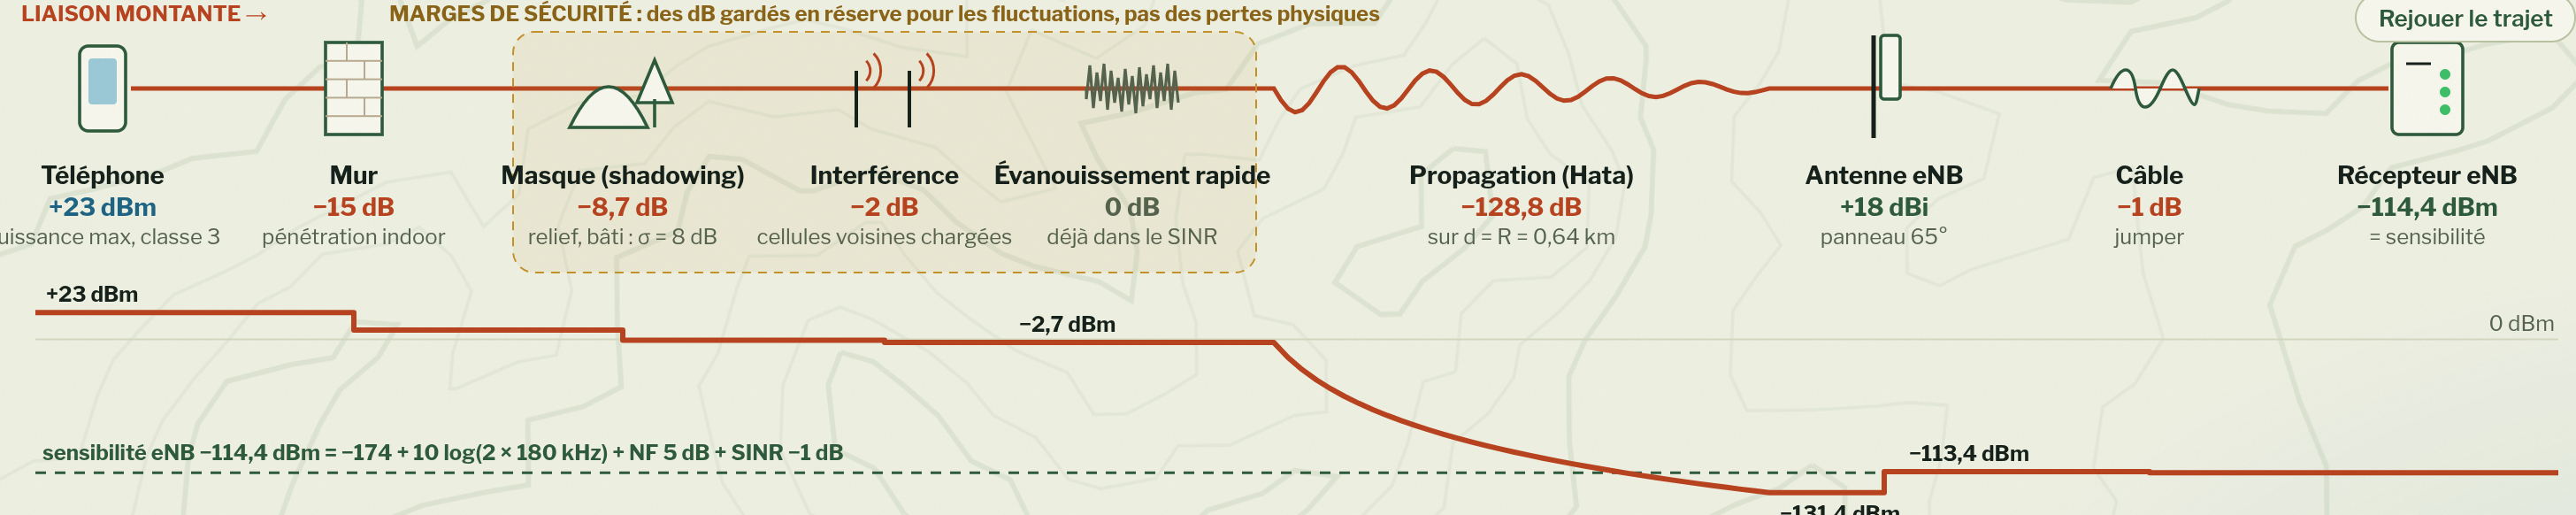
\includegraphics[width=\textwidth]{bilan-chaine.png}
\caption{Bilan de liaison montante, du terminal à la station.}
\label{fig-chaine}
\end{figure}

La \cref{fig-chaine} suit le signal du téléphone (\SI{+23}{\dBm}) jusqu'au récepteur de la station. Les marges (cadre pointillé) ne sont pas des pertes physiques mais des réserves pour les fluctuations ; à la distance $R$, le signal arrive exactement à la sensibilité de \SI{-114,4}{\dBm}.

\subsection{Le modèle de propagation et le rayon}
\label{sec-hata}

À \SI{1800}{\mega\hertz}, nous utilisons le modèle COST-231 Hata~\cite{cost231}, extension du modèle de Hata~\cite{hata1980} (lui-même tiré des mesures d'Okumura~\cite{okumura1968}) à la plage \SIrange{1500}{2000}{\mega\hertz} :
\begin{equation}
  L = 46{,}3 + 33{,}9\log_{10} f - 13{,}82\log_{10} h_b - a(h_m) + (44{,}9 - 6{,}55\log_{10} h_b)\log_{10} d + C_m,
  \label{eq-hata}
\end{equation}
\begin{equation}
  a(h_m) = (1{,}1\log_{10} f - 0{,}7)\,h_m - (1{,}56\log_{10} f - 0{,}8),
\end{equation}
avec $f$ en \si{\mega\hertz}, $d$ en \si{\kilo\metre}, $h_b = \SI{30}{\metre}$, $h_m = \SI{1,5}{\metre}$ et $C_m = \SI{0}{\deci\bel}$ (ville moyenne). À $f = \SI{1720}{\mega\hertz}$ (UL), on obtient $a(h_m) = \SI{0,04}{\deci\bel}$, $L(\SI{1}{\kilo\metre}) = \SI{135,5}{\deci\bel}$ et une pente de \SI{35,2}{\deci\bel} par décade. Le rayon est la distance où l'affaiblissement atteint le MAPL :
\begin{align}
  R &= 10^{(\text{MAPL} - 135{,}5)/35{,}2}, \\
  R_{\text{urbain}} &= 10^{(128{,}8 - 135{,}5)/35{,}2} = \SI{0,64}{\kilo\metre},
  \qquad
  R_{\text{rural}} = 10^{(146{,}6 - 135{,}5)/35{,}2} = \SI{2,06}{\kilo\metre}.
\end{align}
La même formule \enquote{ville moyenne} est utilisée en campagne. C'est un choix prudent, et c'est aussi le réglage par défaut d'Atoll, qui applique cette variante à toutes les classes d'occupation du sol. Le modèle est validé pour $d \geq \SI{1}{\kilo\metre}$ ; le rayon urbain de \SI{0,64}{\kilo\metre} en est une légère extrapolation, que nous acceptons car Atoll utilise le même modèle et que l'écart reste dans l'incertitude de l'effet de masque.

\section{Nombre de sites par la couverture}
\label{sec-sites}

La surface couverte par un site vaut $A_{\text{site}} = k R^2$, avec $k = \tfrac{3\sqrt{3}}{2} \approx 2{,}6$ pour une cellule omnidirectionnelle hexagonale et $k = 1{,}95$ pour un site tri-sectoriel. Le nombre de sites est le rapport de la surface de la zone à celle d'un site. Le gain d'antenne entre dans le bilan, donc chaque configuration a son propre rayon (\cref{tab-sites}).

\begin{table}[H]
\centering
\caption{Sites nécessaires à la couverture selon l'antenne.}
\label{tab-sites}
\begin{tabular}{@{}lccccc@{}}
\toprule
\thead{Configuration} & \thead{$R$ urbain} & \thead{Sites urbains} & \thead{$R$ rural} & \thead{Sites ruraux} & \thead{Total} \\
\midrule
Omni, \SI{11}{\dBi} & \SI{0,41}{\kilo\metre} & 20 & \SI{1,30}{\kilo\metre} & 18 & 38 \\
\rowcolor{mousse!50} \textbf{Tri-secteur \ang{65}, \SI{18}{\dBi}} & \SI{0,64}{\kilo\metre} & \textbf{11} & \SI{2,06}{\kilo\metre} & \textbf{10} & \textbf{21} \\
6 secteurs \ang{33}, \SI{21}{\dBi} & \SI{0,78}{\kilo\metre} & 6 & \SI{2,51}{\kilo\metre} & 5 & 11 \\
\bottomrule
\end{tabular}
\end{table}

Pour la configuration retenue :
\begin{equation}
  N_{\text{urbain}} = \frac{8{,}57}{1{,}95 × 0{,}64^2} = 10{,}7 \;\rightarrow\; 11,
  \qquad
  N_{\text{rural}} = \frac{76{,}95}{1{,}95 × 2{,}06^2} = 9{,}3 \;\rightarrow\; 10.
\end{equation}
La configuration à six secteurs demande moins de sites, mais 66 cellules au lieu de 63 et beaucoup plus de recouvrement en réutilisation~1. Nous gardons le tri-secteur, qui est la configuration recommandée par le cours (un site unique couvre trois cellules avec des antennes sectorielles, pour réduire le nombre de sites à installer et à gérer~\cite{afif2026cours}) et celle des modèles standard d'Atoll.

\begin{figure}[H]
\centering
\begin{subfigure}[b]{0.36\textwidth}\centering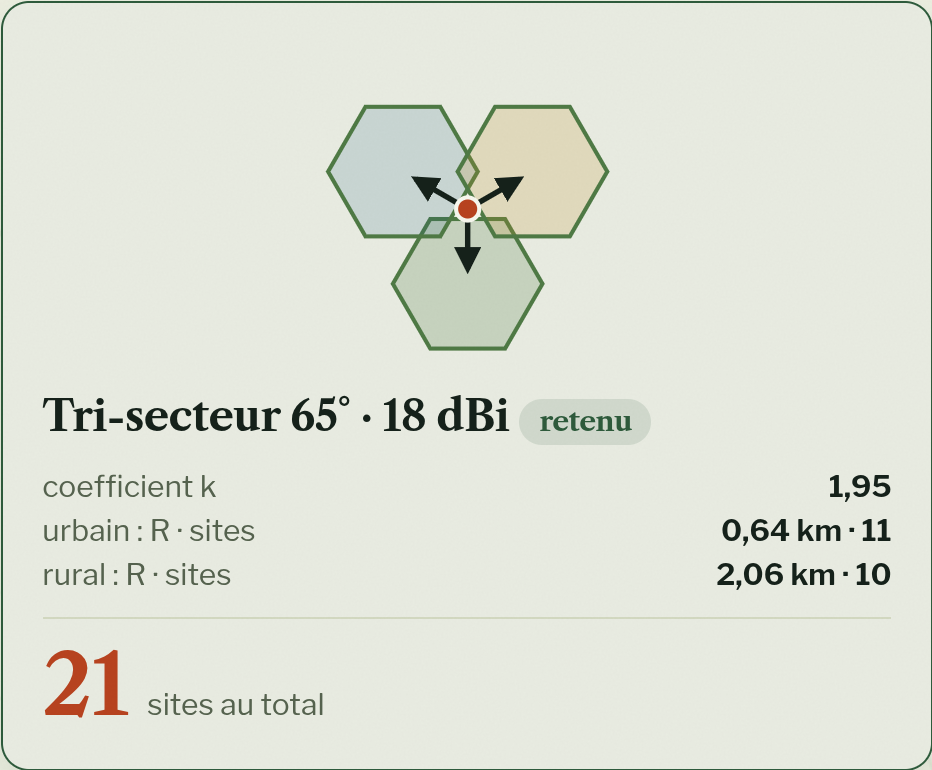
\includegraphics[width=\textwidth]{site-tri.png}\caption{Schéma du site.}\end{subfigure}\hfill
\begin{subfigure}[b]{0.6\textwidth}\centering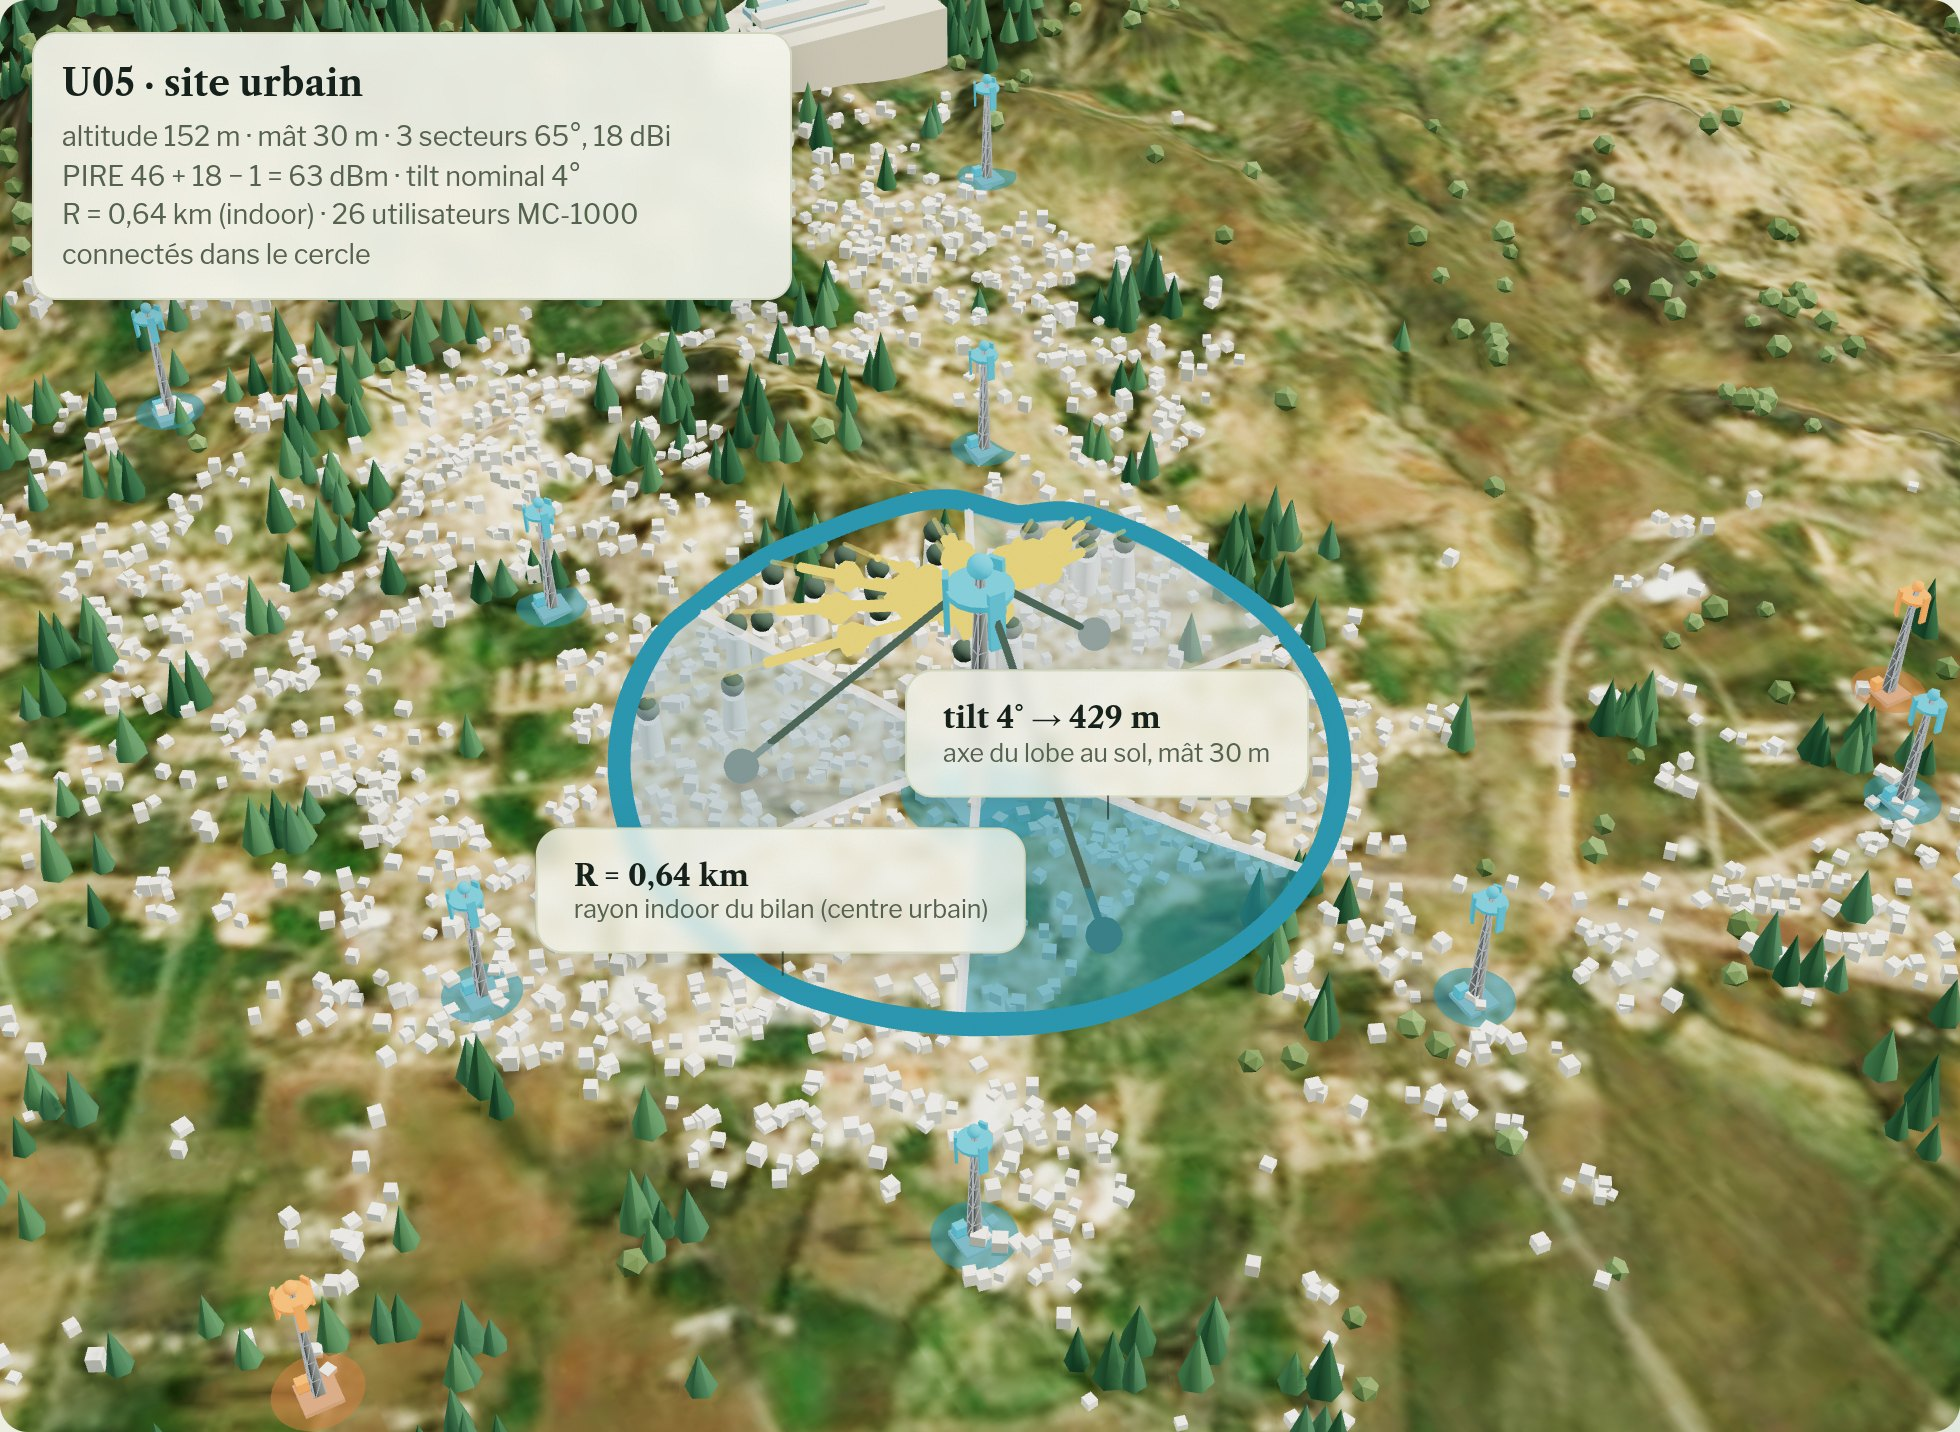
\includegraphics[width=\textwidth]{station-3d.jpg}\caption{Site U05 sur le terrain réel.}\end{subfigure}
\caption{Le site tri-sectoriel retenu.}
\label{fig-site}
\end{figure}

Sur la \cref{fig-site}b, le site U05 porte trois secteurs de \ang{65} ; le cercle a pour rayon $R = \SI{0,64}{\kilo\metre}$. Avec un tilt de \ang{4}, l'axe du lobe touche le sol à $30/\tan 4^\circ \approx \SI{430}{\metre}$.

\section{Dimensionnement par la capacité}
\label{sec-capa}

\subsection{Traduction de la logique GSM en LTE}

Le sujet décrit le dimensionnement par la capacité dans la logique GSM : fréquences par cellule, canaux de trafic égaux aux canaux totaux moins deux canaux de signalisation, abonnés par cellule par la loi d'Erlang~B, puis cellules et sites. Le LTE n'alloue pas de circuits mais des ressources temps-fréquence partagées. Nous gardons la même suite d'étapes en traduisant chaque notion (\cref{tab-gsm-lte}).

\begin{table}[H]
\centering
\caption{Étapes du sujet (GSM) et leur équivalent LTE.}
\label{tab-gsm-lte}
\begin{tabularx}{\textwidth}{@{}LLr@{}}
\toprule
\thead{Étape du sujet (GSM)} & \thead{Équivalent LTE} & \thead{Valeur} \\
\midrule
Fréquences par cellule & une porteuse de \SI{20}{\mega\hertz}, réutilisation 1 & 100 RB \\
Canaux de trafic = total $-$ 2 de signalisation & éléments de ressource (RE) par RB, moins le canal de contrôle (PDCCH) et les signaux de référence & DL 120/168 ; UL 144/168 \\
Abonnés par cellule (Erlang B, GoS) & débit de la cellule × charge maximale \SI{80}{\percent} / débit d'un abonné & 272 \\
Cellules = abonnés / abonnés par cellule & idem & 14 \\
Sites = cellules / 3 & idem (tri-secteur) & \textbf{5} \\
\bottomrule
\end{tabularx}
\end{table}

\begin{cours}{capacité d'un système cellulaire}
La capacité intrinsèque vaut $C_{\text{int}} = \dfrac{n}{K \cdot B}$, où $n$ est le nombre de canaux par porteuse, $K$ la taille du motif et $B$ la bande duplex d'un canal. En GSM ($n = 8$, $B = \SI{0,4}{\mega\hertz}$, $K = 9$), $C_{\text{int}} = 2{,}2$ canaux par cellule et par MHz. La capacité du réseau est $\dfrac{n\,\eta}{K \cdot B \cdot \pi R^2}$ en \si{Er\per\hertz\per\kilo\metre\squared}, où le rendement $\eta$ est le rapport entre canaux de trafic et canaux totaux~\cite{afif2026cours}.
\application Le rendement $\eta$ du cours est la ligne \enquote{canaux de trafic} du \cref{tab-gsm-lte}. Pour une porteuse GSM, $\eta = (8 - 2)/8 = 0{,}75$. En LTE, $\eta = 120/168 = 0{,}71$ en DL et $144/168 = 0{,}86$ en UL : la signalisation consomme une part comparable de la ressource. La formule montre aussi les deux leviers de capacité que nous utilisons : un motif $K$ petit (ici $K = 1$, \cref{sec-reuse}) et des cellules plus petites (rayon $R$).
\end{cours}

\subsection{Débit moyen d'une cellule}

Le débit d'une cellule dépend de la qualité de signal de ses utilisateurs. Nous avons appliqué la formule de C/I du cours (six interféreurs, \cref{sec-reuse}) en \emph{chaque point} d'une cellule hexagonale, converti chaque valeur en bearer Atoll grâce aux seuils de SINR, puis moyenné l'efficacité spectrale obtenue : \SI{1,894}{bit} par élément de ressource. Avec 120 RE utiles par RB et par milliseconde, 100 RB et le facteur applicatif de 0,95 d'Atoll,
\begin{equation}
  D_{\text{cellule}} = 1{,}894 × 120 × 100 × \num{1000} × 0{,}95 \approx \SI{21,6}{\Mbps} \text{ en DL}
\end{equation}
(\SI{25,9}{\Mbps} en UL). Le gain du MIMO, possible au-dessus de \SI{12}{\deci\bel} sur \SI{24}{\percent} de la cellule, n'est pas compté, ce qui rend l'estimation prudente.

\subsection{Demande et nombre de sites}

\begin{align}
  \text{abonnés LTE (centre)} &= \num{13590} × 0{,}939 × 0{,}30 × 0{,}93 \approx \num{3560}, \\
  \text{demande DL à l'heure chargée} &= \num{3560} × \SI{63,3}{\kbps} \approx \SI{225}{\Mbps}, \\
  \text{abonnés par cellule} &= \frac{\SI{21,6}{\Mbps} × 0{,}80}{\SI{63,3}{\kbps}} \approx 272, \\
  \text{cellules} &= \num{3560} / 272 \approx 13{,}1 \;\rightarrow\; 14, \qquad \text{sites} = 14 / 3 \;\rightarrow\; \mathbf{5}.
\end{align}
La capacité ne demande que 5 sites dans le centre, contre 11 pour la couverture indoor : la ville est aujourd'hui limitée par la couverture. Au rythme de croissance observé (+\SI{40}{\percent} en deux ans, soit $1{,}4^{5/2} \approx 2{,}3$ en cinq ans), le besoin en capacité atteindrait 11 sites dans cinq ans, ce que le réseau dimensionné par la couverture peut absorber. En campagne, la capacité demanderait 4 sites, contre 10 pour la couverture.

\section{Motif de réutilisation et plan de fréquences}
\label{sec-reuse}

\begin{cours}{réutilisation et rapport C/I}
Le nombre de cellules d'un motif vaut $K = i^2 + ij + j^2$ ($i$, $j$ entiers). La distance de réutilisation et le rapport de réutilisation co-canal sont
\begin{equation}
  D = \sqrt{3K}\,R, \qquad q = \frac{D}{R}.
\end{equation}
Avec $K_1$ cellules co-canal au premier anneau, $C \propto R^{-\alpha}$ et, pour un mobile en bord de cellule, $I_k \propto (D - R)^{-\alpha}$ :
\begin{equation}
  \frac{C}{I} = \frac{1}{\sum_{k=1}^{K_1} (q - 1)^{-\alpha}} = \frac{(q - 1)^{\alpha}}{6} \quad (K_1 = 6).
  \label{eq-ci}
\end{equation}
Seuils donnés dans le cours : \SI{18}{\deci\bel} en FDMA ; \SI{9}{\deci\bel} en GSM, d'où un motif de 7 ou 9 cellules ; \SI{3}{\deci\bel}, d'où un motif de 3 ou 4 cellules. Le système doit fonctionner avec le C/I le plus faible possible, pour réduire $D$ et la taille du motif~\cite{afif2026cours}.
\application L'indice du milieu $\alpha$ est la pente de notre modèle de Hata, $\alpha = 3{,}52$. Le seuil LTE est celui du bearer~4, \SI{-1}{\deci\bel}. Le \cref{tab-reuse} applique la formule~\eqref{eq-ci} à chaque motif.
\end{cours}

\begin{table}[H]
\centering
\caption{C/I dans le pire cas du cours selon le motif ($\alpha = 3{,}52$).}
\label{tab-reuse}
\small\setlength{\tabcolsep}{4.5pt}
\begin{tabular}{@{}ccccccc@{}}
\toprule
\thead{$K$} & \thead{$(i, j)$} & \thead{$q$} & \thead{C/I pire cas} & \thead{GSM ($\geq$ \SI{9}{\deci\bel})} & \thead{LTE ($\geq$ \SI{-1}{\deci\bel})} & \thead{Spectre par cellule} \\
\midrule
\rowcolor{mousse!50} \textbf{1} & (1, 0) & 1,73 & \SI{-12,6}{\deci\bel} & non & non & \textbf{\SI{20,0}{\mega\hertz}} \\
3 & (1, 1) & 3,00 & \SI{2,8}{\deci\bel} & non & oui & \SI{6,7}{\mega\hertz} \\
4 & (2, 0) & 3,46 & \SI{6,0}{\deci\bel} & non & oui & \SI{5,0}{\mega\hertz} \\
7 & (2, 1) & 4,58 & \SI{11,7}{\deci\bel} & oui & oui & \SI{2,9}{\mega\hertz} \\
9 & (3, 0) & 5,20 & \SI{14,2}{\deci\bel} & oui & oui & \SI{2,2}{\mega\hertz} \\
\bottomrule
\end{tabular}
\end{table}

Avec notre pente, nous retrouvons les ordres de grandeur du cours : le seuil GSM de \SI{9}{\deci\bel} conduit à $K = 7$ ou 9, et un seuil de \SI{3}{\deci\bel} à $K = 3$ ou 4. Pour le LTE (\SI{-1}{\deci\bel}), ce pire cas conduirait à $K = 3$. Il suppose cependant que l'utilisateur est en bord de cellule et que les six interféreurs sont tous au plus près en même temps. En calculant le C/I en chaque point de la cellule (\cref{fig-ci}), seuls \SI{8,4}{\percent} de la surface passent sous \SI{-1}{\deci\bel}, et la médiane est de \SI{5,4}{\deci\bel}. Comme le LTE adapte la modulation et le codage au SINR de chaque utilisateur, il tolère une qualité faible en bord de cellule. Nous retenons donc $K = 1$ : chaque cellule dispose des \SI{20}{\mega\hertz}, trois fois plus de spectre qu'avec $K = 3$. C'est la règle du cours (C/I le plus faible possible, donc motif le plus petit) appliquée jusqu'à $K = 1$ ; l'interférence en bord de cellule est ensuite traitée par la planification (tilt, azimut).

\begin{figure}[H]
\centering
\begin{subfigure}[b]{0.38\textwidth}\centering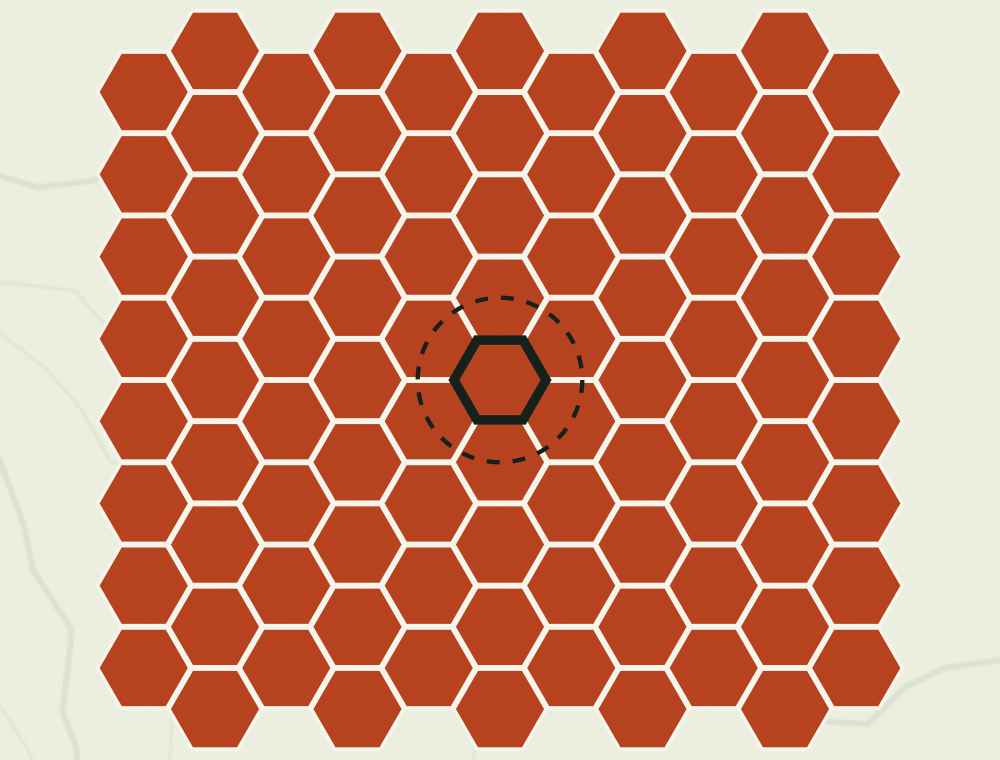
\includegraphics[width=\textwidth]{reuse-k1.png}\caption{Interféreurs co-canal, $K = 1$.}\end{subfigure}\hfill
\begin{subfigure}[b]{0.58\textwidth}\centering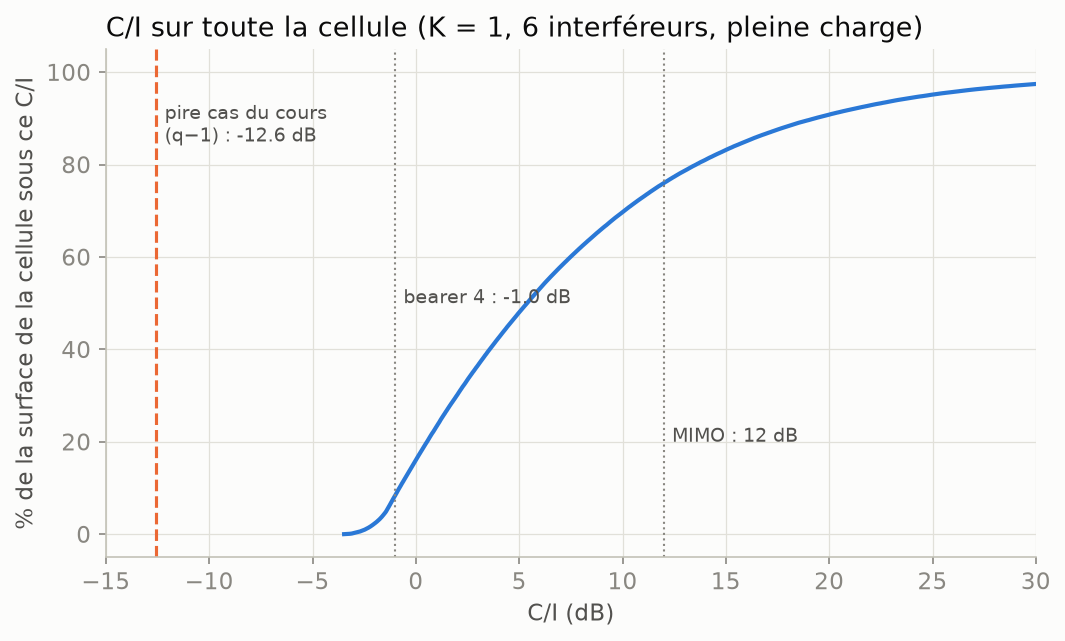
\includegraphics[width=\textwidth]{fig3_CI_cellule.png}\caption{C/I en chaque point de la cellule.}\end{subfigure}
\caption{C/I en réutilisation 1 : pire cas et distribution sur la cellule.}
\label{fig-ci}
\end{figure}

\paragraph{Plan de fréquences.} Toutes les cellules utilisent la même porteuse de \SI{20}{\mega\hertz} (EARFCN 1300, 100 RB). En LTE, la planification porte alors sur les identifiants physiques de cellule (PCI) : le site numéro $s$ reçoit les PCI $3s$, $3s + 1$ et $3s + 2$. Les trois secteurs d'un site ont ainsi des valeurs modulo 3 différentes, et leurs signaux de référence ne se superposent pas en fréquence~\cite{sesia2011}.

\section{Synthèse et choix de la bande}
\label{sec-800-1800}

\begin{table}[H]
\centering
\caption{Nombre de sites retenu par zone.}
\label{tab-sites-final}
\begin{tabular}{@{}lcccl@{}}
\toprule
\thead{Zone} & \thead{Couverture} & \thead{Capacité} & \thead{Retenu} & \thead{Contrainte} \\
\midrule
Centre urbain & 11 & 5 & 11 & couverture indoor \\
Rural & 10 & 4 & 10 & couverture outdoor \\
\midrule
\textbf{Total} & & & \textbf{21} & \\
\bottomrule
\end{tabular}
\end{table}

Dans chaque zone, le nombre retenu est le plus grand des deux besoins. Le même calcul a été mené à \SI{800}{\mega\hertz} (bande 20, \SI{10}{\mega\hertz}, modèle d'Okumura-Hata), avec les mêmes marges, les mêmes antennes et la même puissance par RB (\cref{tab-800-1800}).

\begin{table}[H]
\centering
\caption{Bandes 800 et \SI{1800}{\mega\hertz} comparées.}
\label{tab-800-1800}
\small\setlength{\tabcolsep}{5pt}
\begin{tabular}{@{}lccccc@{}}
\toprule
\thead{Bande} & \thead{$R$ urbain} & \thead{$R$ rural} & \thead{Sites\\couverture} & \thead{Total\\aujourd'hui} & \thead{Total dans\\5 ans} \\
\midrule
\SI{800}{\mega\hertz}, \SI{10}{\mega\hertz} & \SI{1,22}{\kilo\metre} & \SI{3,91}{\kilo\metre} & 6 & 12 & 24 \\
\SI{1800}{\mega\hertz}, \SI{20}{\mega\hertz} & \SI{0,64}{\kilo\metre} & \SI{2,06}{\kilo\metre} & 21 & 21 & \textbf{21} \\
\bottomrule
\end{tabular}
\end{table}

Le \SI{800}{\mega\hertz} demande moins de sites aujourd'hui (12 contre 21), car il porte plus loin. Avec \SI{10}{\mega\hertz} seulement, la ville y est limitée par la capacité (9 sites aujourd'hui), et il faudrait 24 sites dans cinq ans avec un trafic multiplié par 2,3. À \SI{1800}{\mega\hertz}, les 21 sites restent suffisants. Le \SI{800}{\mega\hertz} reste une bonne couche de couverture, que nous citons en perspective (\cref{ch-disc}).

\section{Le plan nominal}
\label{sec-nominal}

Les sites sont placés automatiquement sur une grille hexagonale de distance inter-sites $1{,}5\,R$ : \SI{0,96}{\kilo\metre} en ville et \SI{3,1}{\kilo\metre} en campagne, sans aucun site sur le massif. Les effets de bord donnent 20 sites (10 urbains, 10 ruraux) au lieu des 21 de la formule. Nous n'avons rien corrigé à la main : deux sites ruraux (R01, R02) tombent près de sites urbains et R07 tombe sur le flanc du massif. Ce plan brut est le réseau initial d'Atoll ; ses défauts sont corrigés au \cref{ch-opt}, avec une mesure avant et après chaque action.

\begin{figure}[H]
\centering
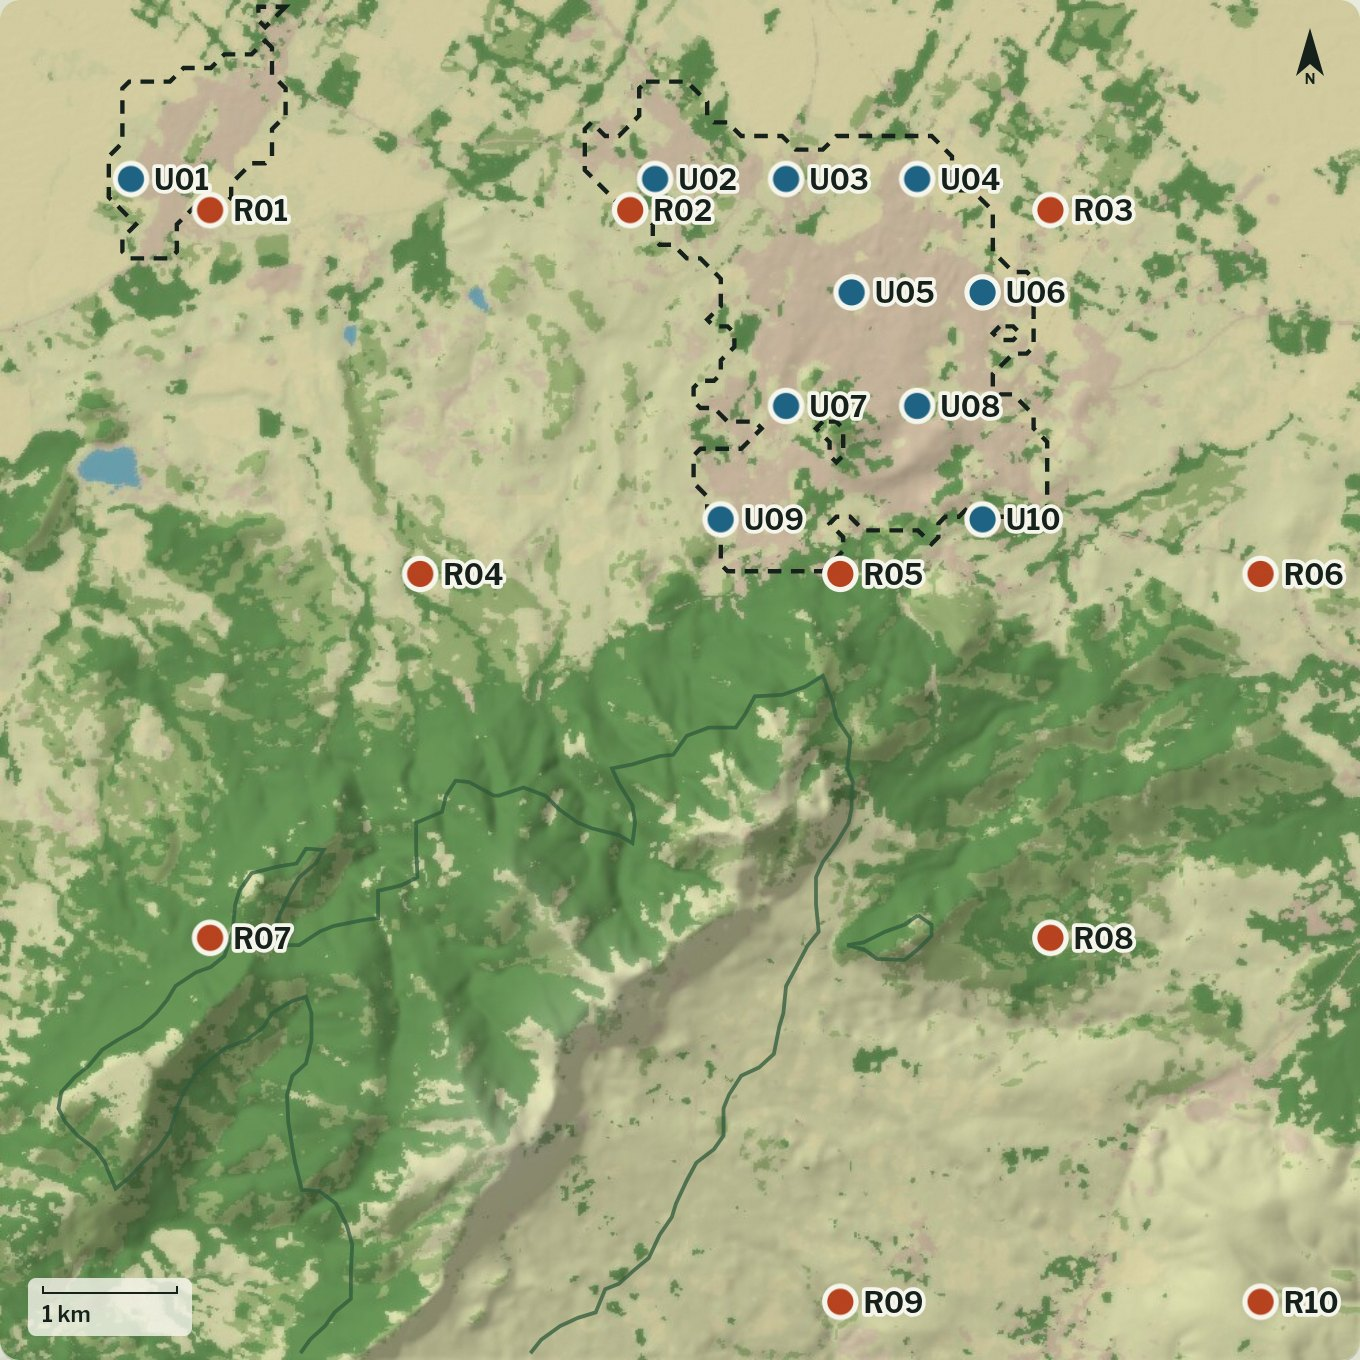
\includegraphics[width=0.6\textwidth]{plan-nominal.jpg}
\caption{Plan nominal (20 sites).}
\label{fig-nominal}
\end{figure}

Sur la \cref{fig-nominal}, les sites urbains sont en bleu et les sites ruraux en terre cuite ; leurs coordonnées sont données en \cref{ann-sites}.

\begin{retenir}
Le bilan de liaison donne un rayon de \SI{0,64}{\kilo\metre} en ville et \SI{2,06}{\kilo\metre} en campagne, limité par la liaison montante. La couverture impose 21 sites tri-sectoriels ; la capacité n'en demanderait que 5 dans le centre. La réutilisation retenue est $K = 1$, avec une porteuse de \SI{20}{\mega\hertz}.
\end{retenir}

\chapter{Mise en œuvre dans Atoll}
\label{ch-atoll}

Ce chapitre décrit la construction, dans Atoll 3.3, du réseau calculé à l'Étape 1, avec la même zone, le même modèle de propagation, les mêmes équipements et les mêmes marges. Les captures de chaque réglage sont fournies avec le projet.

\section{Les cartes}

Trois couches ont été préparées à partir des données ouvertes et importées dans un projet en WGS~84 / UTM~32N :

\begin{table}[H]
\centering
\caption{Couches géographiques importées.}
\label{tab-cartes}
\begin{tabularx}{\textwidth}{@{}llLl@{}}
\toprule
\thead{Couche} & \thead{Grille} & \thead{Contenu} & \thead{Source} \\
\midrule
Relief (MNT) & \num{400} × \num{400}, \SI{25}{\metre} & altitude de 101 à \SI{1238}{\metre} & \cite{copernicusdem} \\
Occupation du sol & \num{1000} × \num{1000}, \SI{10}{\metre} & 8 classes WorldCover & \cite{worldcover2022} \\
Population & \num{100} × \num{100}, \SI{100}{\metre} & densité en \si{hab\per\kilo\metre\squared}, total \num{25360} & \cite{worldpop2018} \\
\bottomrule
\end{tabularx}
\end{table}

Deux difficultés ont été rencontrées. Le lecteur TIFF d'Atoll 3.3 refusait nos fichiers (\enquote{Unsupported bit depth}) : il a fallu les réécrire en entiers non compressés, pixels contigus, sans palette, avec un fichier de géoréférencement \texttt{.tfw}. Ensuite, la carte de population importée comme \enquote{nombre par pixel} apparaissait 100 fois trop grande (\num{285700} au lieu de \SI{2857}{hab\per\kilo\metre\squared} au centre) : elle doit être déclarée comme une densité. Chaque valeur importée a été vérifiée au survol contre le fichier source.

\section{Propagation et occupation du sol}

Le modèle retenu dans Atoll est Cost-Hata, la même formule que l'Étape 1 (équation~\eqref{eq-hata}), avec l'option \enquote{Add diffraction loss} activée. Atoll calcule alors l'obstruction du relief entre l'antenne et chaque point, que la formule de Hata seule ignore ; c'est cette option qui fait apparaître l'ombre du massif. Nous n'avons pas retenu le modèle SPM : ses coefficients se calibrent sur des mesures terrain que nous n'avons pas, et ses valeurs par défaut sont celles de Hata.

Atoll applique l'effet de masque et la pénétration indoor \emph{par classe d'occupation du sol}. Nous avons saisi trois niveaux d'écart-type cohérents avec l'Étape 1 : \SI{8}{\deci\bel} pour le bâti, \SI{7}{\deci\bel} pour la forêt et les arbustes (la végétation fait varier davantage le signal que le terrain ouvert), \SI{6}{\deci\bel} pour les classes ouvertes. La pénétration indoor est de \SI{15}{\deci\bel} pour le bâti et \SI{10}{\deci\bel} pour les autres classes à \SI{1800}{\mega\hertz}.

\section{Les modèles de station}

Les modèles de station fournis par Atoll sont prévus pour \SI{10}{\mega\hertz} en bande~1 (\SI{2100}{\mega\hertz}). Nous avons créé deux modèles \enquote{20 MHz -- B3 -- Urbain / Rural (3 secteurs)} : bande~3 en \SI{20}{\mega\hertz}, \SI{46}{\dBm}, modèle Cost-Hata, pertes de \SI{1}{\deci\bel}, facteur de bruit de \SI{5}{\deci\bel}, charge maximale de \SI{80}{\percent}, hauteur de \SI{30}{\metre}, tilt électrique de \ang{4} (urbain) ou \ang{2} (rural). Le RS EPRE affiché par Atoll, \SI{15,4}{\dBm}, est cohérent avec les \SI{15,2}{\dBm} calculés : la puissance de \SI{46}{\dBm} est bien réglée. L'antenne est le modèle \enquote{65deg 18dBi} de la bibliothèque d'Atoll, défini à \SI{2100}{\mega\hertz} ; nous n'avons pas utilisé de version à \SI{1800}{\mega\hertz}.

\begin{figure}[H]
\centering
\begin{subfigure}[b]{0.3\textwidth}\centering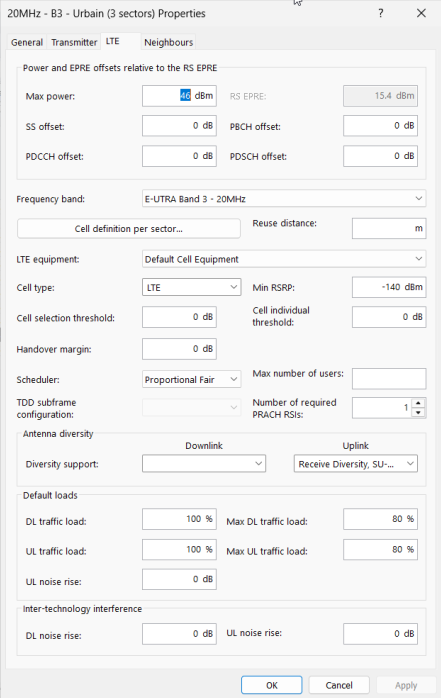
\includegraphics[width=\textwidth]{template_lte.png}\caption{Modèle de station : bande 3, \SI{20}{\mega\hertz}, \SI{46}{\dBm}.}\end{subfigure}\hfill
\begin{subfigure}[b]{0.66\textwidth}\centering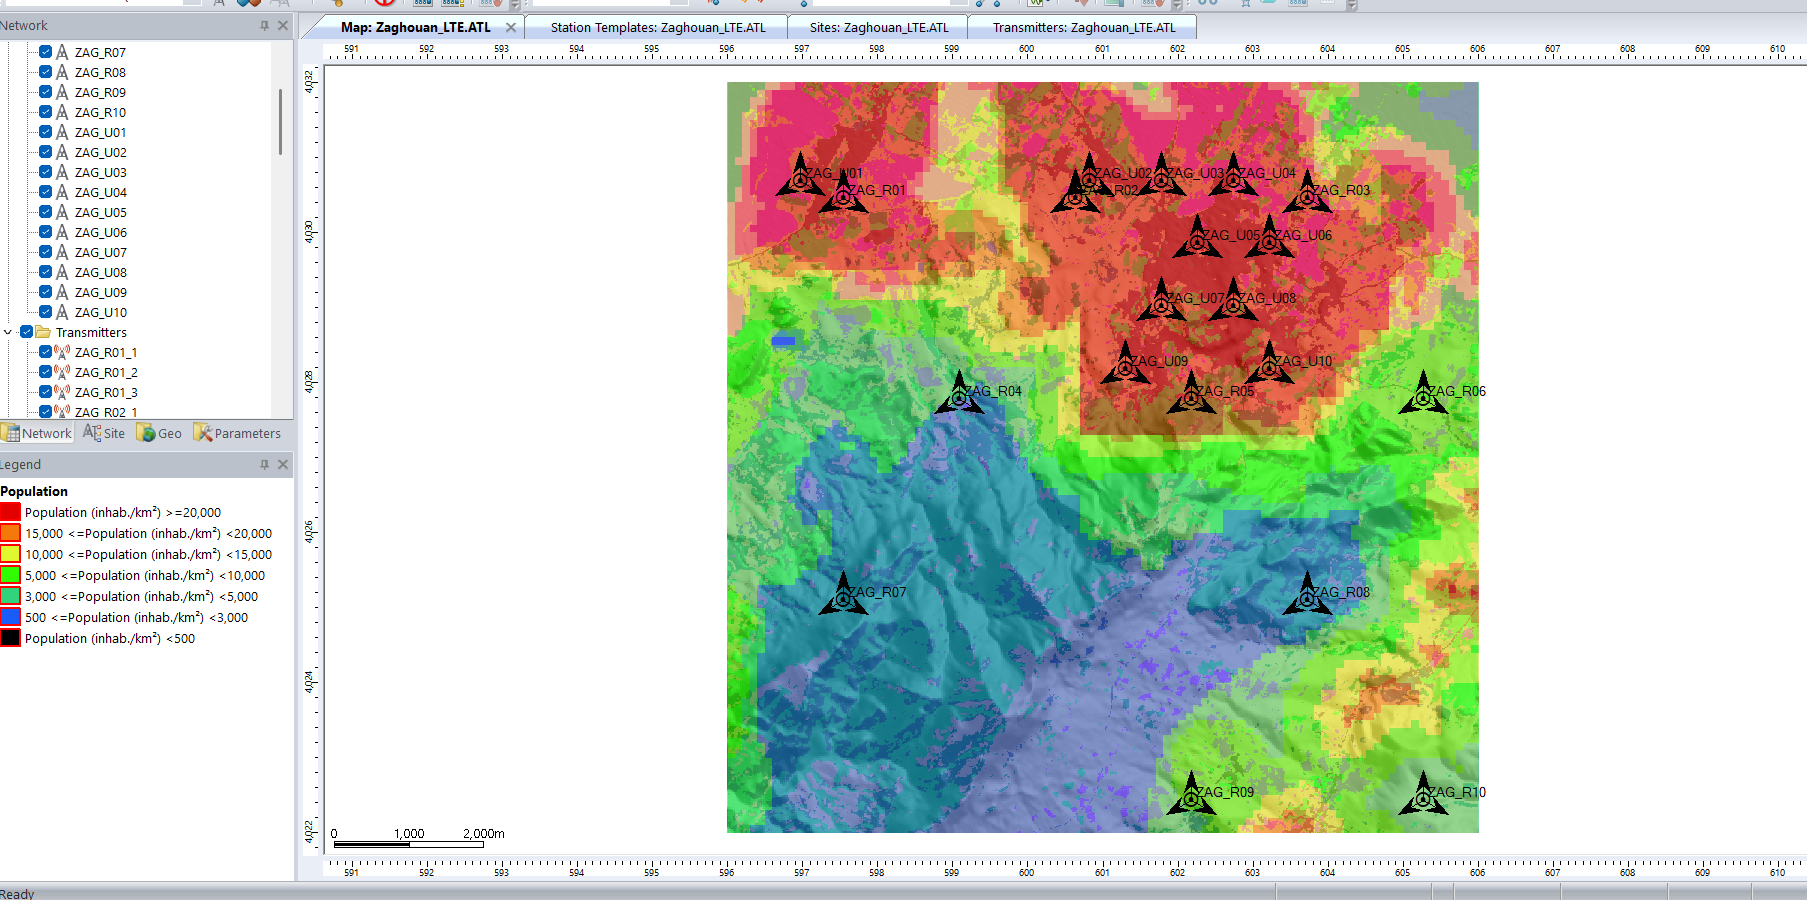
\includegraphics[width=\textwidth]{S02-05_reseau_complet.png}\caption{Le réseau initial : 20 sites, 60 émetteurs.}\end{subfigure}
\caption{Le réseau de l'Étape 1 construit dans Atoll.}
\label{fig-atoll-reseau}
\end{figure}

\section{Le réseau initial}

Les 20 sites du plan nominal (\cref{sec-nominal}) ont été collés dans la table des sites depuis le fichier de coordonnées produit par l'Étape 1 ; Atoll a lu leurs altitudes sur le MNT, cohérentes avec les nôtres. Chaque site a reçu une station de trois secteurs, d'azimuts \ang{0}, \ang{120} et \ang{240}, soit \textbf{60 émetteurs}. Le critère de couverture est un seuil unique sur le niveau du signal de référence (RSRP), déduit du même bilan de liaison. Atoll ajoute lui-même, par classe, l'effet de masque et la pénétration indoor ; le seuil ne doit donc contenir que la marge d'interférence. L'affaiblissement limite en UL vaut alors $P_{\text{UE}} + G - L - S - M_{\text{interf}}$, et le RSRP reçu à cet affaiblissement vaut $\text{RS EPRE} + G - L$ moins cet affaiblissement. Les gains d'antenne s'annulent :
\begin{equation}
  \text{RSRP}_{\min} = \text{RS EPRE} - P_{\text{UE}} + S + M_{\text{interf}} = 15{,}2 - 23 - 114{,}4 + 2 \approx \SI{-120}{\dBm}.
\end{equation}

\section{Le trafic}

Le trafic des simulations Monte-Carlo suit la population : une carte de densité d'utilisateurs a été créée à partir de notre carte de population (\enquote{1 habitant = 1 utilisateur potentiel}), avec tous les utilisateurs actifs en UL et en DL. Chaque simulation applique ensuite un facteur d'échelle qui fixe le nombre d'utilisateurs tirés. Le mélange de services, de mobilités et de terminaux est une hypothèse de travail :

\begin{table}[H]
\centering
\caption{Paramètres de trafic des simulations Monte-Carlo.}
\label{tab-mix}
\begin{tabularx}{\textwidth}{@{}lL@{}}
\toprule
\thead{Paramètre} & \thead{Valeur} \\
\midrule
Services & High Speed Internet \SI{60}{\percent}, Mobile Internet Access \SI{25}{\percent}, VoIP \SI{15}{\percent} \\
Mobilités & piéton \SI{70}{\percent}, \SI{50}{\kilo\metre\per\hour} \SI{20}{\percent}, fixe \SI{10}{\percent} \\
Terminal & MIMO 2 × 2 (\SI{100}{\percent}) \\
Part d'utilisateurs à l'intérieur & \SI{70}{\percent} dans le bâti, \SI{0}{\percent} ailleurs \\
\bottomrule
\end{tabularx}
\end{table}

\begin{retenir}
Le réseau d'Atoll est exactement celui de l'Étape 1 : mêmes 20 sites, même modèle Hata, même puissance, mêmes antennes, mêmes marges. La seule différence voulue est la diffraction sur le relief réel.
\end{retenir}

\chapter{Prédictions de couverture et de débit}
\label{ch-pred}

Ce chapitre présente les livrables de prédiction du sujet sur le réseau initial (20 sites) : niveau de signal, couverture par émetteur et recouvrement, qualité C/(I+N), débits DL et UL. Chaque carte est l'export d'Atoll avec sa légende. Pour comparer chaque résultat aux objectifs \emph{par zone}, nous avons exporté les prédictions en raster (\SI{50}{\metre}) et écrit un script qui les croise avec les zones de l'Étape 1, en surface et en population. Le même script mesure ensuite chaque action d'optimisation.

\section{Niveau de signal}
\label{sec-signal}

La prédiction \enquote{Coverage by Signal Level (DL)} est calculée avec le seuil de \SI{-120}{\dBm}, l'effet de masque activé avec une probabilité de \SI{86}{\percent} au bord de la cellule (celle de la formule de Jakes, \cref{tab-jakes}) et une résolution de \SI{50}{\metre}. Deux versions ont été produites : indoor (objectif urbain) et outdoor (objectif rural).

\begin{figure}[H]
\centering
\begin{subfigure}[b]{0.58\textwidth}\centering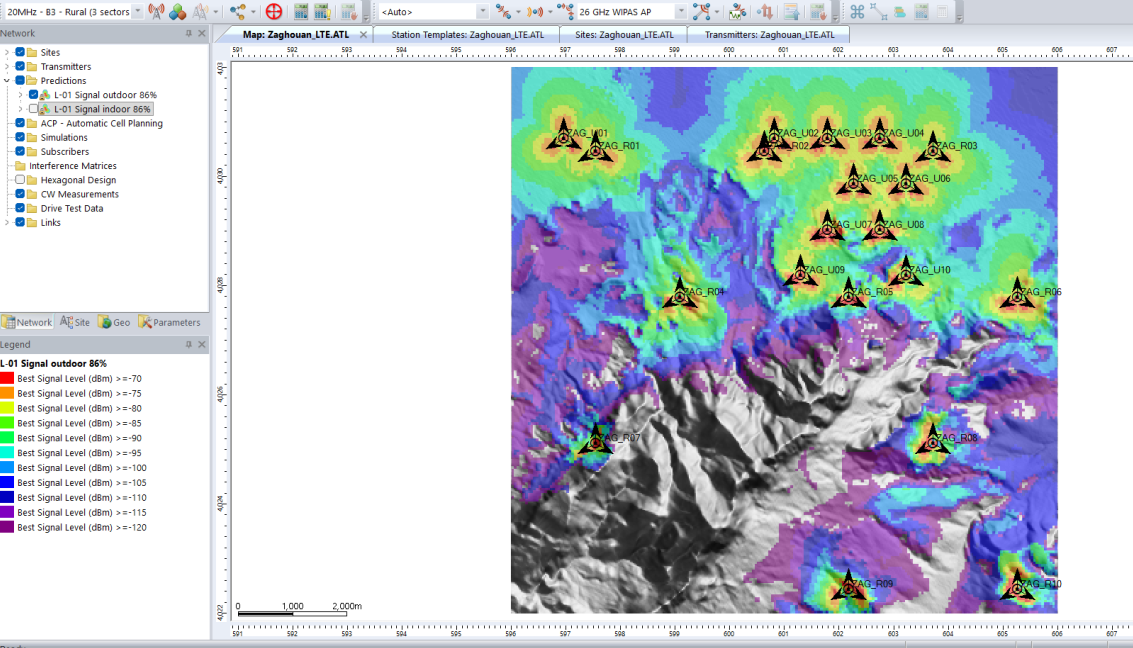
\includegraphics[width=\textwidth]{L-01_signal_outdoor_86_initial.png}\caption{Carte et légende Atoll, outdoor.}\end{subfigure}\hfill
\begin{subfigure}[b]{0.4\textwidth}\centering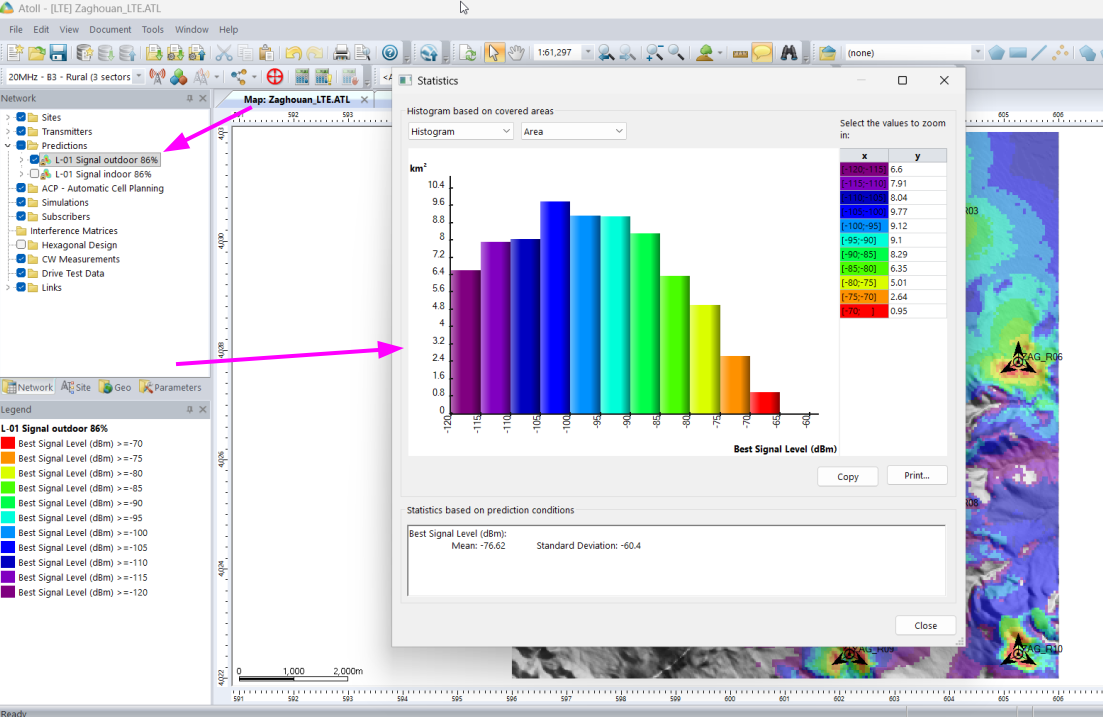
\includegraphics[width=\textwidth]{L-02_histogramme_outdoor_initial.png}\caption{Histogramme (surface par classe).}\end{subfigure}
\caption{Niveau de signal du réseau initial (outdoor).}
\label{fig-l1}
\end{figure}

L'histogramme donne \SI{59,1}{\kilo\metre\squared} au-dessus de \SI{-120}{\dBm} en indoor et \SI{73,8}{\kilo\metre\squared} en outdoor, sur les \SI{100}{\kilo\metre\squared} de la carte (massif compris). Par zone :

\begin{table}[H]
\centering
\caption{Couverture par niveau de signal du réseau initial.}
\label{tab-l1}
\small\setlength{\tabcolsep}{5pt}
\begin{tabular}{@{}lccccc@{}}
\toprule
\thead{Zone} & \thead{Mode} & \thead{Surface\\couverte} & \thead{Population\\couverte} & \thead{Objectif} & \thead{Verdict} \\
\midrule
Centre urbain & indoor & \SI{99,5}{\percent} & \SI{99,6}{\percent} & \SI{95}{\percent} & \ok \\
Rural & outdoor & \SI{83,4}{\percent} & \SI{95,4}{\percent} & \SI{95}{\percent} & \ko{} ($-11{,}6$ pts) \\
Massif & outdoor & \SI{7}{\percent} & -- & aucun & -- \\
\bottomrule
\end{tabular}
\end{table}

La ville est entièrement couverte en indoor. En campagne, il manque 11,6 points. Les trous se situent derrière le massif (\cref{fig-trous}) : le coin sud-ouest, où R07, placé sur le flanc, est masqué ; le pied est de la crête ; le sud-est, entre R08, R09 et R10. Ces zones sont peu peuplées : \SI{95,4}{\percent} des habitants ruraux sont couverts. L'objectif étant fixé en surface, il n'est pas atteint.

\begin{figure}[H]
\centering
\begin{subfigure}[b]{0.49\textwidth}\centering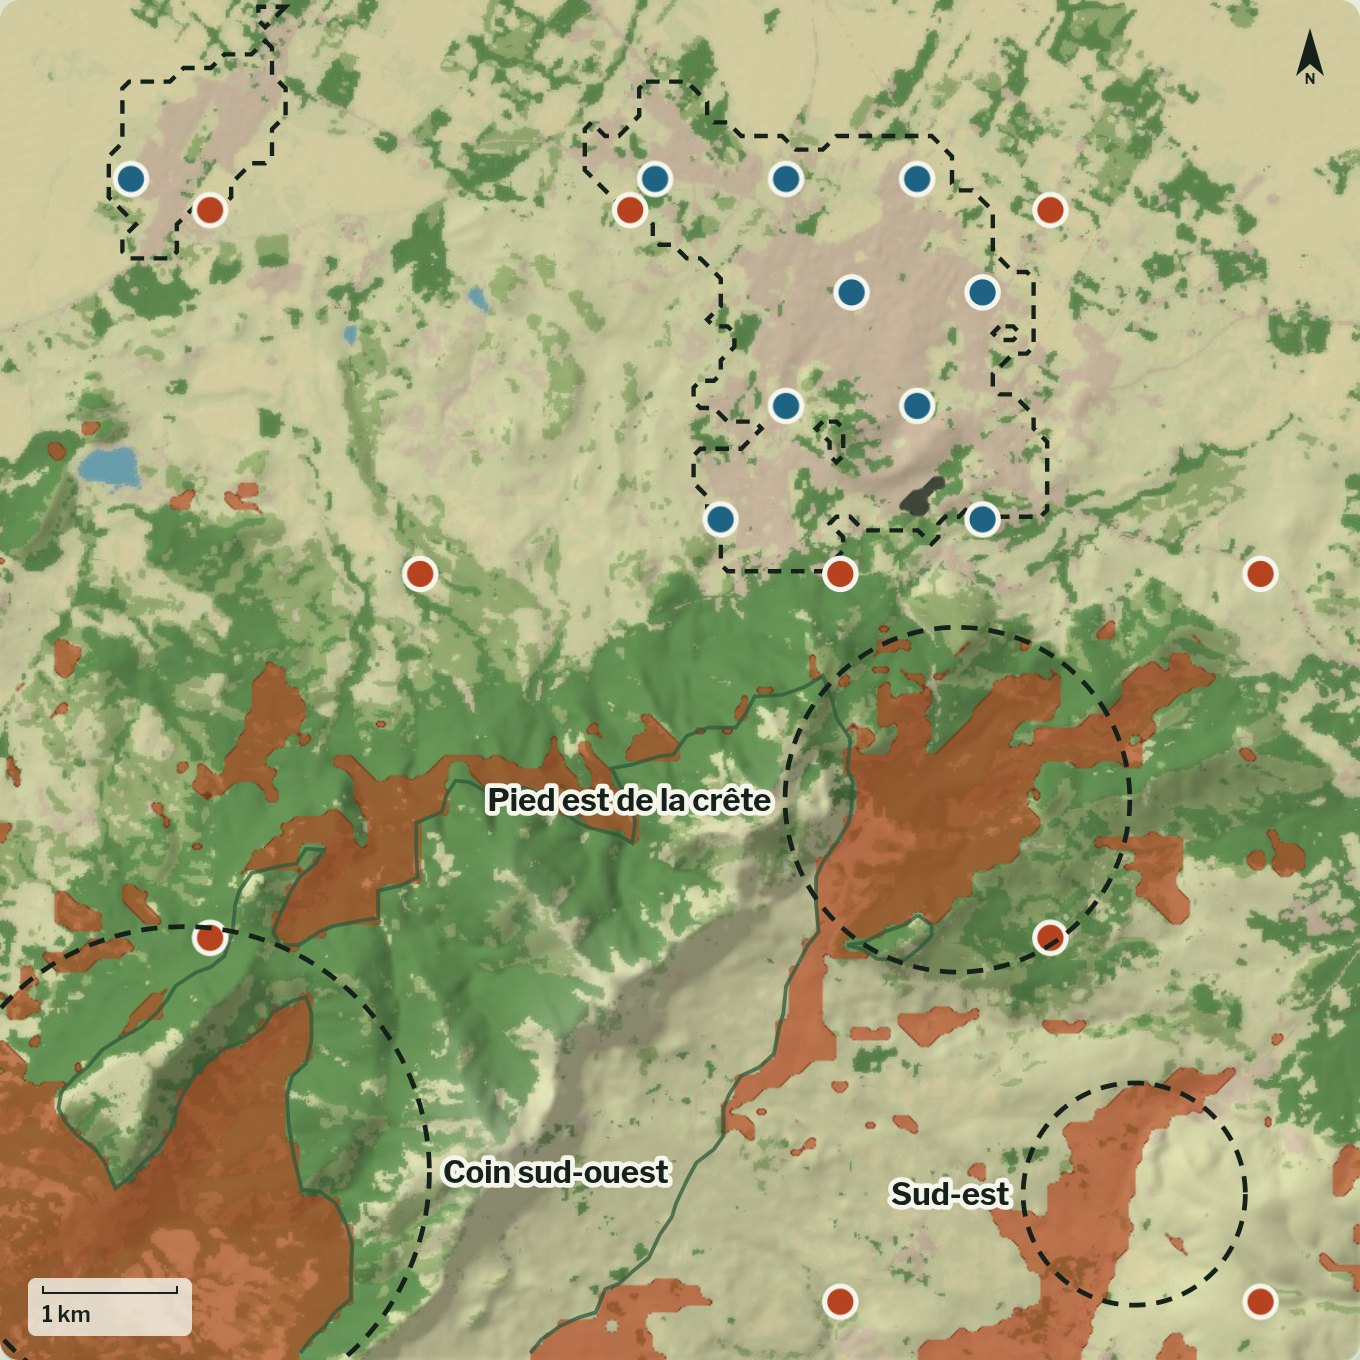
\includegraphics[width=\textwidth]{trous-initial.jpg}\caption{Trous de couverture rurale (en rouge).}\end{subfigure}\hfill
\begin{subfigure}[b]{0.49\textwidth}\centering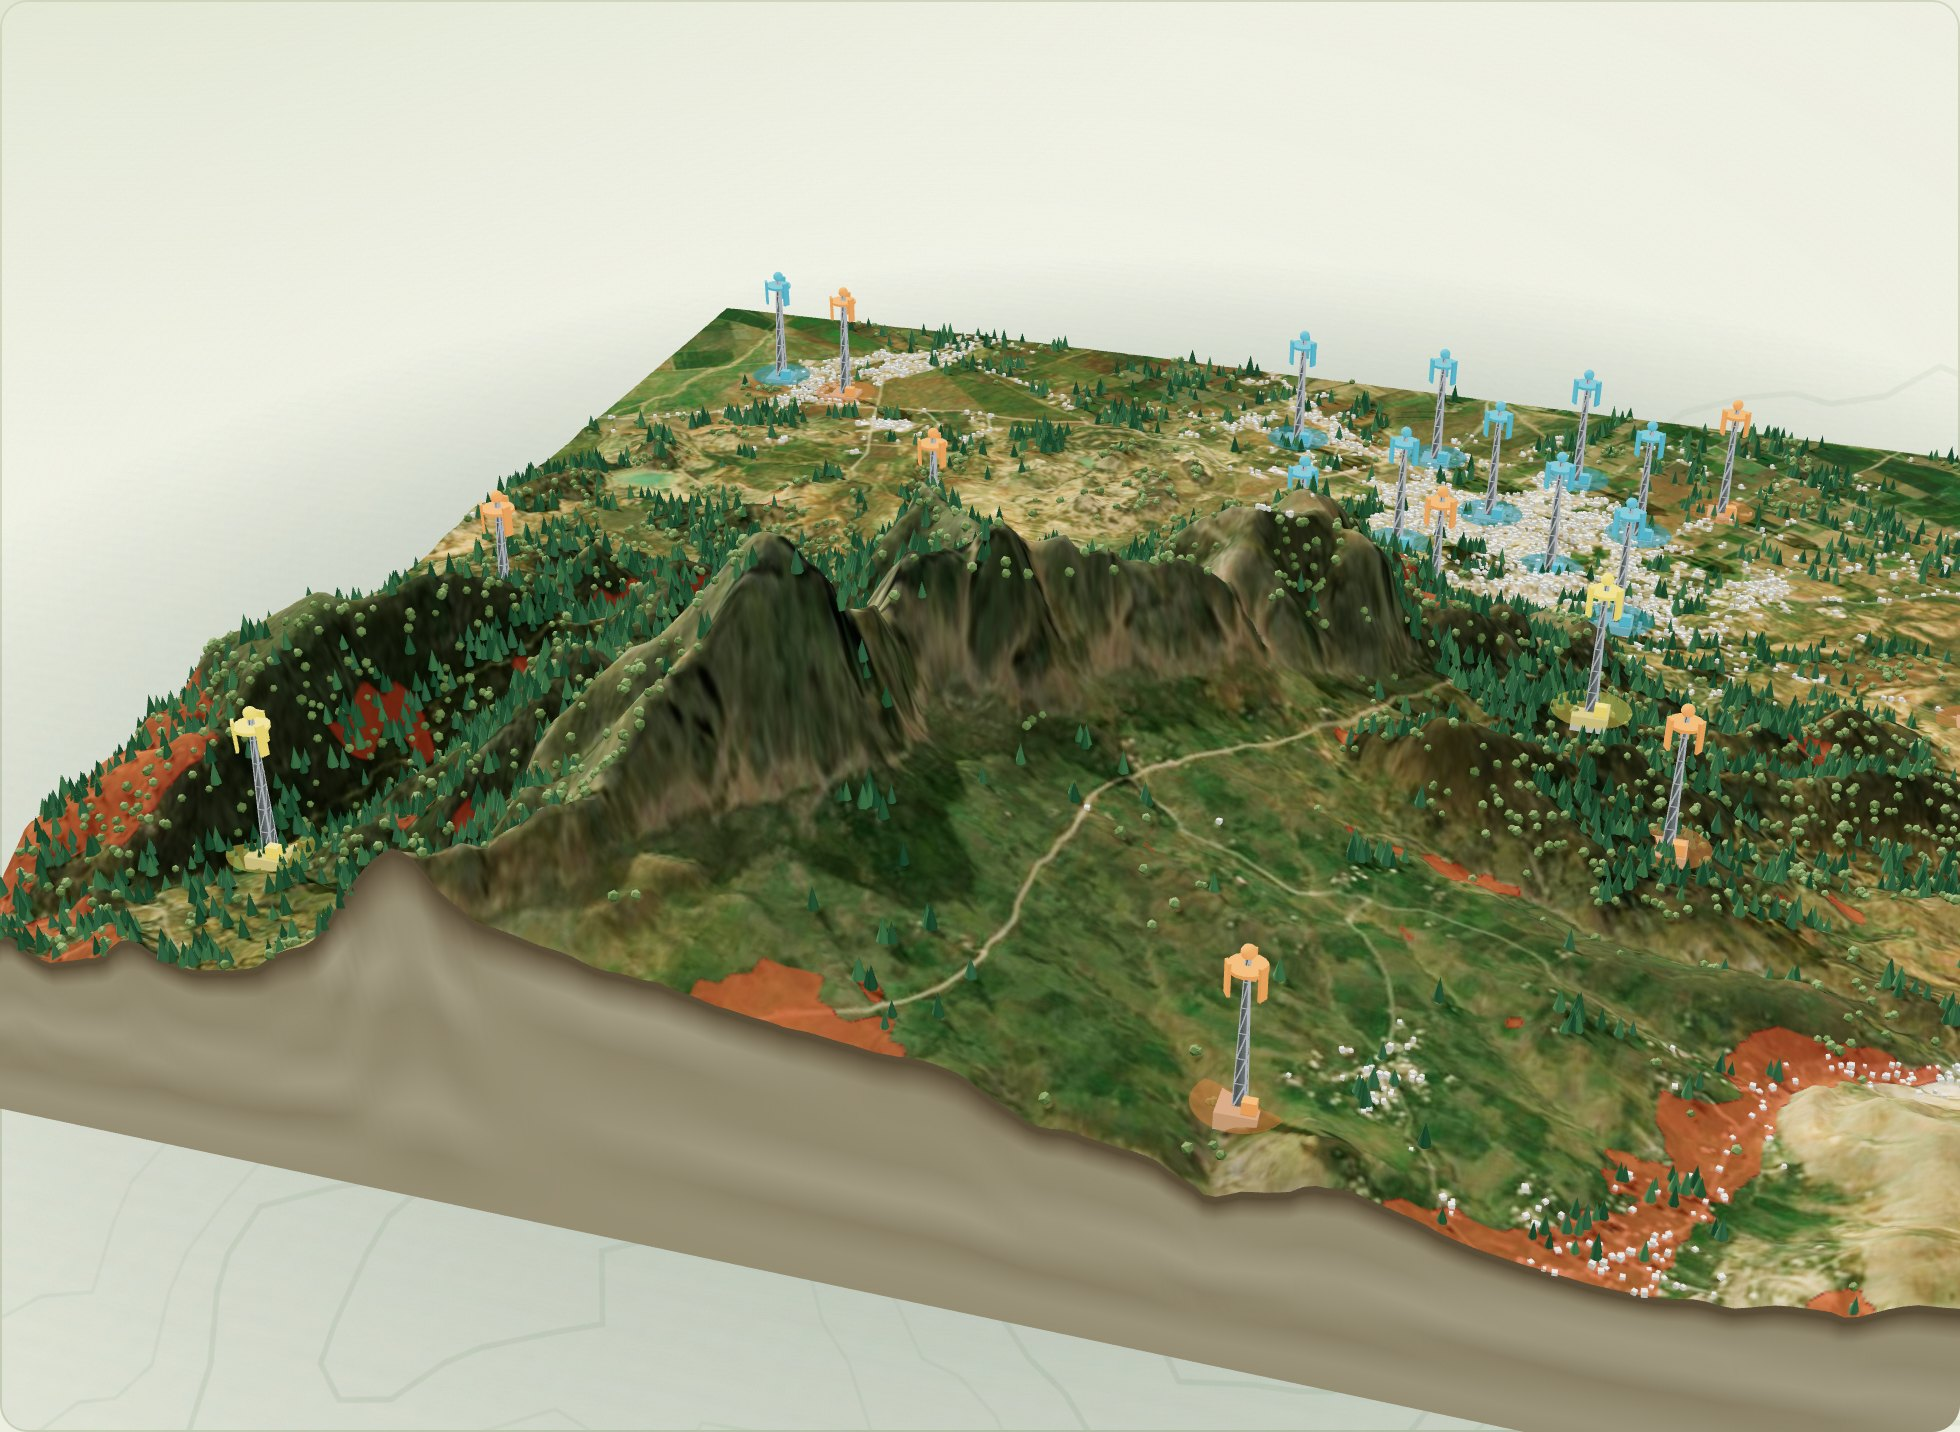
\includegraphics[width=\textwidth]{ombre-initial.jpg}\caption{Les mêmes trous drapés sur le relief réel.}\end{subfigure}
\caption{Trous de couverture rurale du réseau initial.}
\label{fig-trous}
\end{figure}

Les trous (en rouge) sont dans l'ombre de la crête. C'est la diffraction sur le relief, ignorée par la formule de Hata seule, qui les fait apparaître.

\section{Couverture par émetteur et recouvrement}
\label{sec-recouvrement}

La carte par émetteur (\cref{fig-l4}a) montre la zone servie par chaque cellule : les sites ruraux placés en hauteur (R04, R06) servent loin dans la plaine. La carte de recouvrement (\cref{fig-l4}b) compte, en chaque point, le nombre d'émetteurs reçus à moins de \SI{5}{\deci\bel} du meilleur.

\begin{figure}[H]
\centering
\begin{subfigure}[b]{0.49\textwidth}\centering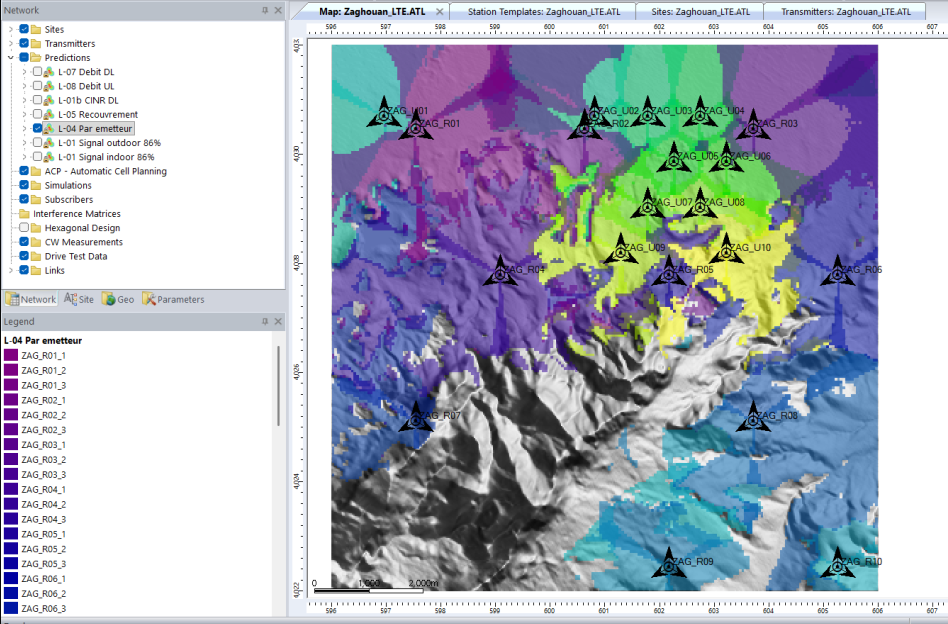
\includegraphics[width=\textwidth]{L-04_par_emetteur_initial.png}\caption{Couverture par émetteur.}\end{subfigure}\hfill
\begin{subfigure}[b]{0.49\textwidth}\centering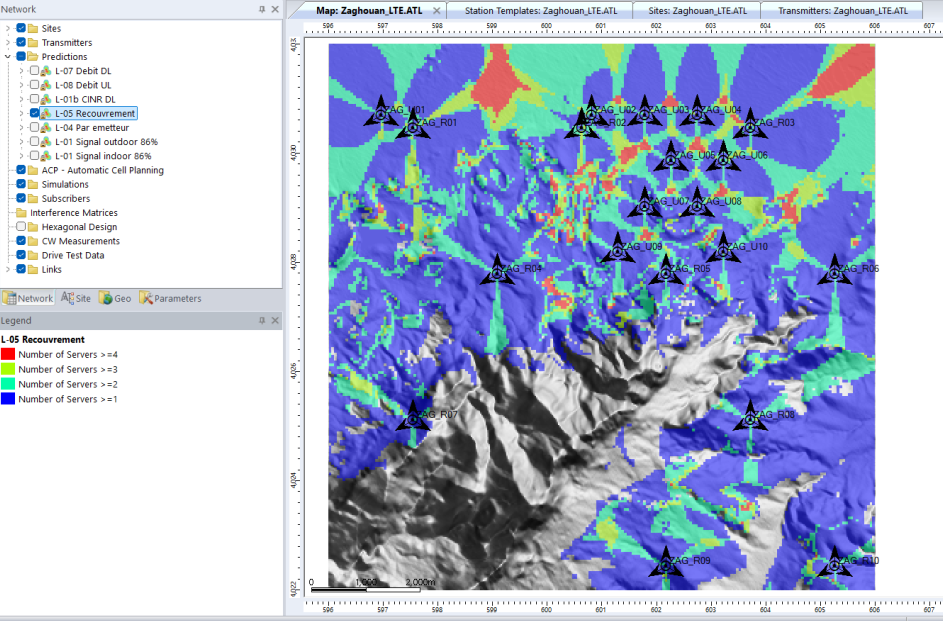
\includegraphics[width=\textwidth]{L-05_recouvrement_initial.png}\caption{Recouvrement (marge \SI{5}{\deci\bel}) et légende.}\end{subfigure}
\caption{Couverture par émetteur et recouvrement du réseau initial.}
\label{fig-l4}
\end{figure}

\begin{table}[H]
\centering
\caption{Histogramme de recouvrement du réseau initial.}
\label{tab-l5}
\begin{tabular}{@{}lccccc@{}}
\toprule
\thead{Nombre de serveurs} & \thead{1} & \thead{2} & \thead{3} & \thead{$\geq$ 4} & \thead{Total couvert} \\
\midrule
Surface (\si{\kilo\metre\squared}) & 48,85 & 17,83 & 4,70 & \textcolor{terre}{\textbf{2,39}} & 73,77 \\
\bottomrule
\end{tabular}
\end{table}

Avec une marge de \SI{5}{\deci\bel}, \SI{34}{\percent} de la surface couverte reçoit au moins deux serveurs à \SI{5}{\deci\bel} près (en moyenne 1,49 serveur). C'est utile pour le handover, mais en réutilisation~1 chaque serveur en trop est un interféreur. Les zones à quatre serveurs ou plus se situent dans la ville, entre U02 et U04, autour de U05 à U08 et près de R02.

\section{Qualité du signal : C/(I+N)}
\label{sec-cinr}

Un point couvert doit aussi recevoir un signal utile qui domine l'interférence. La prédiction C/(I+N) en DL (\cref{fig-cinr}) utilise la charge écrite dans la table des cellules, par défaut \SI{100}{\percent} pour les 60 cellules.

\begin{figure}[H]
\centering
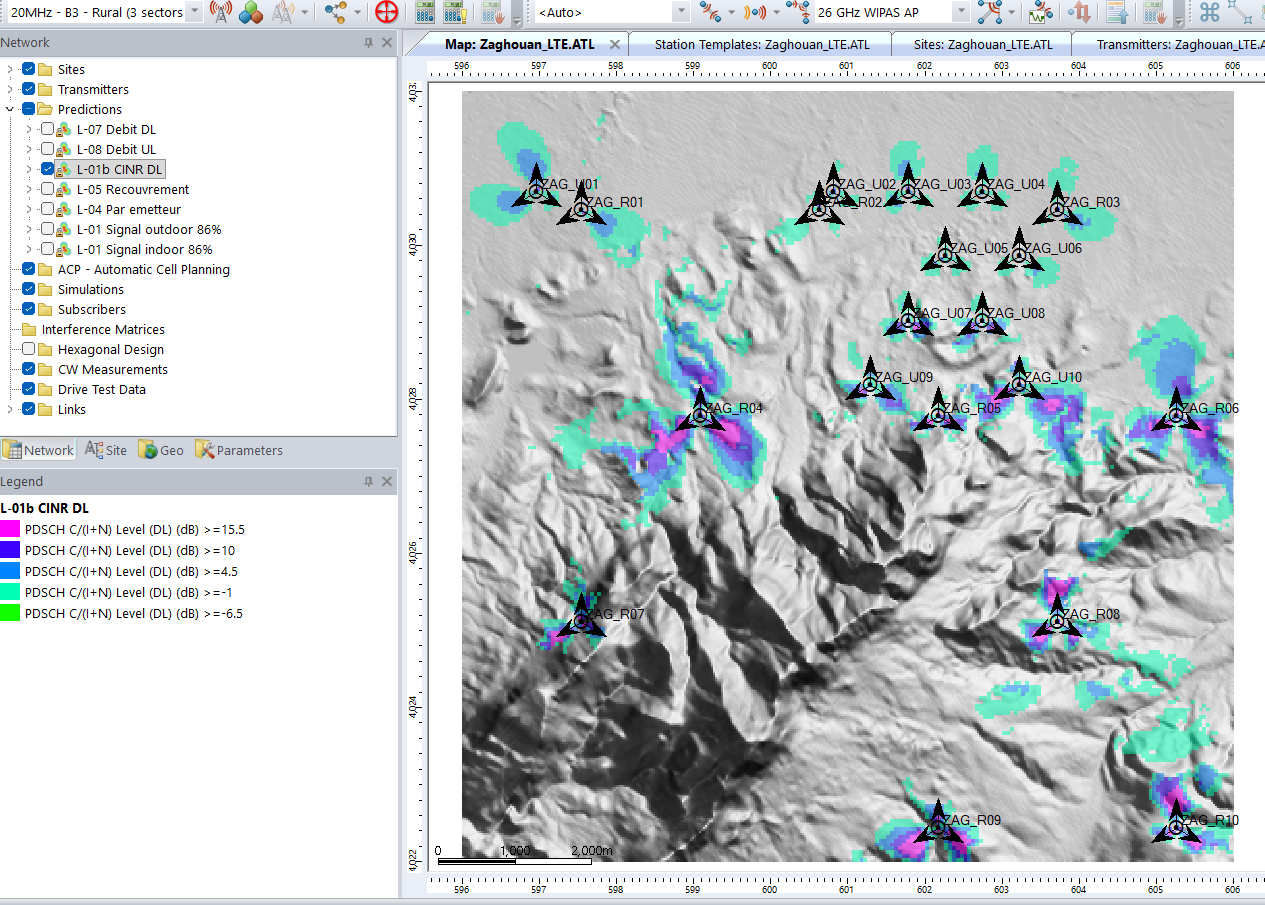
\includegraphics[width=0.7\textwidth]{L-01b_CINR_DL_initial.png}
\caption{C/(I+N) en DL du réseau initial (charge \SI{100}{\percent}).}
\label{fig-cinr}
\end{figure}

Sur la \cref{fig-cinr}, les zones blanches n'ont aucun bearer utilisable pour le service. Seuls \SI{13,1}{\kilo\metre\squared} atteignent \SI{-1}{\deci\bel}, le seuil du bearer~4 (moyenne \SI{4,9}{\deci\bel}). Le recouvrement l'explique : avec quatre serveurs reçus au même niveau, le signal utile fait face à trois interféreurs, soit $C/I = 1/3 \approx \SI{-5}{\deci\bel}$. C'est la limite de $K = 1$ annoncée par la formule du cours (formule~\eqref{eq-ci}, pire cas \SI{-12,6}{\deci\bel}), cette fois sur un relief réel. Trois causes ont été examinées séparément :
\begin{enumerate}
  \item \textbf{la géométrie des sites urbains} (recouvrement, tilt trop faible), traitée au \cref{ch-opt} ;
  \item \textbf{la charge de \SI{100}{\percent}} sur les 60 cellules, très pessimiste, remplacée plus loin par la charge simulée (\cref{sec-charge}) ;
  \item \textbf{la marge d'effet de masque} de \SI{86}{\percent}, qu'Atoll applique aussi au C/(I+N) : une prédiction sans cette marge agrandit nettement les zones de bonne qualité, mais les trous entre sites urbains restent. La cause principale est donc la géométrie.
\end{enumerate}
La même table des cellules fixe une montée du bruit en UL de \SI{0}{\deci\bel} : les prédictions UL ignorent donc l'interférence montante. Les cartes DL sont ainsi pessimistes et les cartes UL optimistes.

\section{Débits DL et UL}
\label{sec-debits}

Les prédictions de débit utilisent le service High Speed Internet (notre objectif de bord de cellule), un terminal MIMO, la mobilité piéton et les mêmes conditions d'effet de masque que le niveau de signal. Nous affichons le débit \emph{applicatif}, reçu par l'application après les erreurs de transmission et le facteur de 0,95 ; c'est lui qui se compare aux \SI{1024}{\kbps}. Les légendes commencent à l'objectif (\SI{1024}{\kbps} en DL, \SI{128}{\kbps} en UL), si bien qu'un point blanc dans la zone couverte est un point où l'objectif n'est pas atteint.

\begin{figure}[H]
\centering
\begin{subfigure}[b]{0.49\textwidth}\centering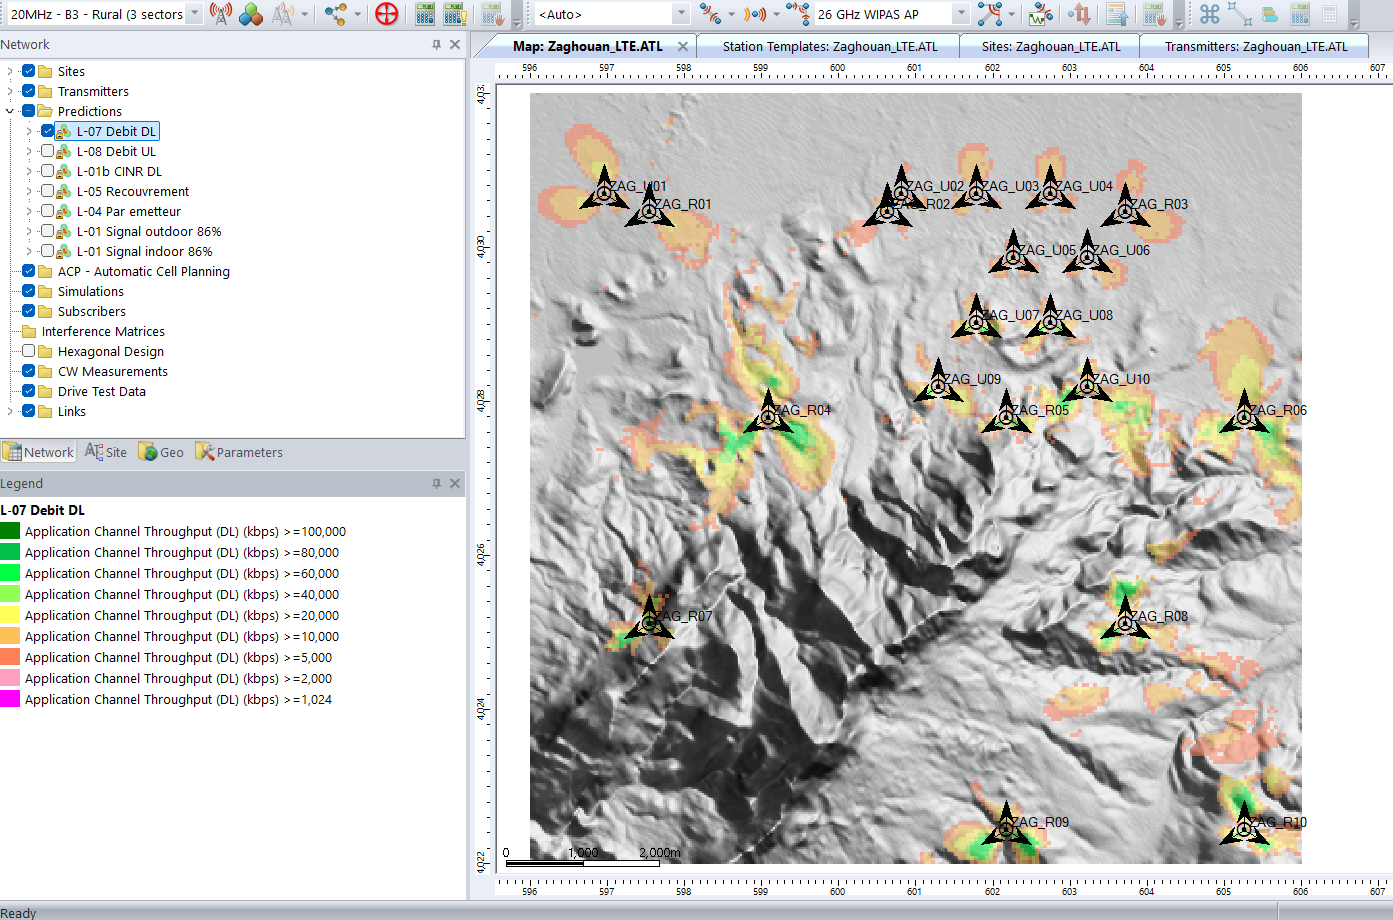
\includegraphics[width=\textwidth]{L-07_debit_DL_initial.png}\caption{Débit DL et légende.}\end{subfigure}\hfill
\begin{subfigure}[b]{0.49\textwidth}\centering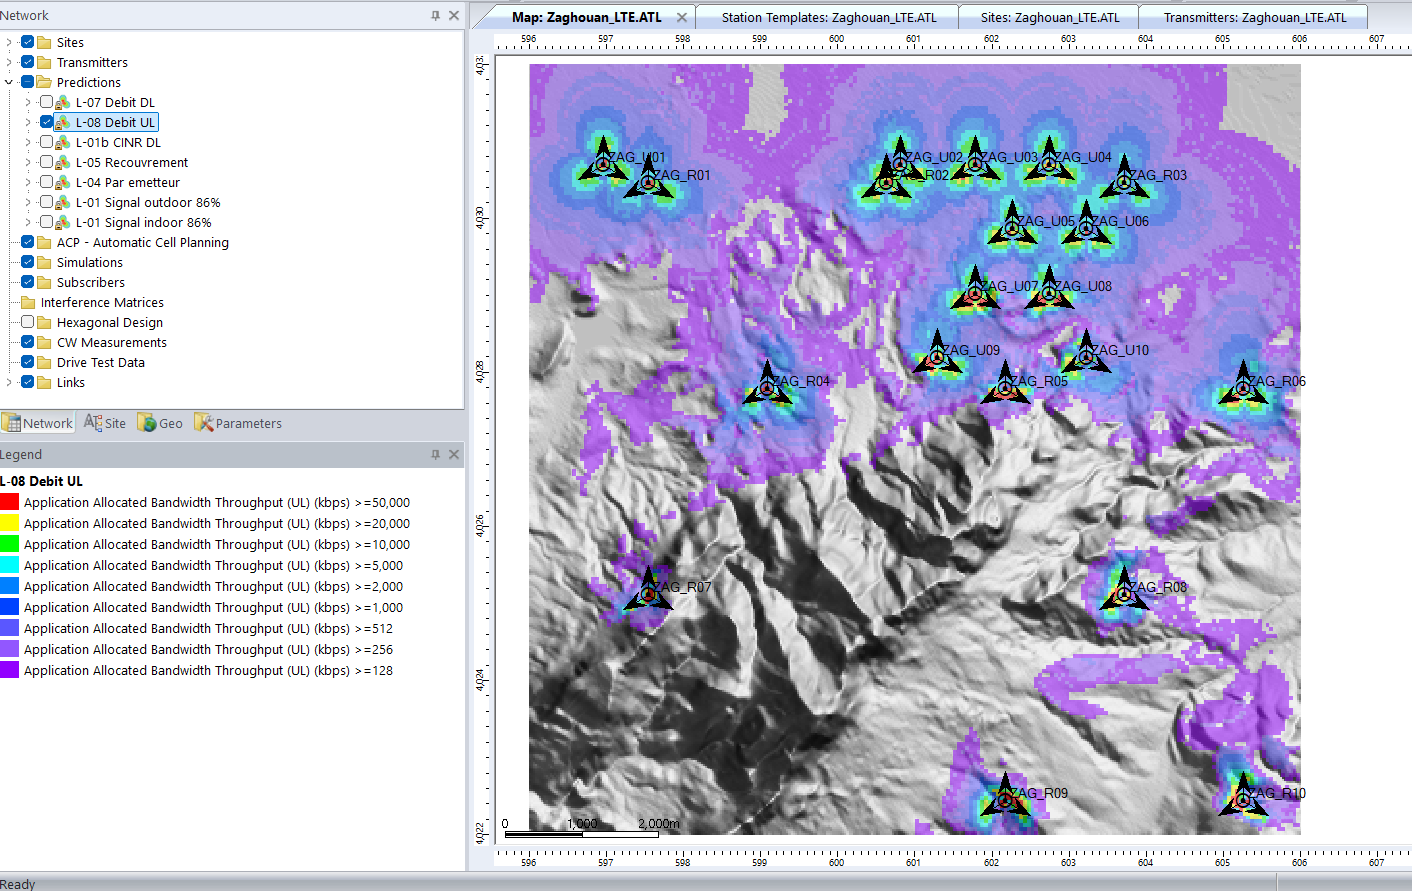
\includegraphics[width=\textwidth]{L-08_debit_UL_initial.png}\caption{Débit UL et légende.}\end{subfigure}
\caption{Débits applicatifs du réseau initial (charge \SI{100}{\percent}).}
\label{fig-debits}
\end{figure}

\begin{itemize}
  \item DL : \SI{13,1}{\kilo\metre\squared} reçoivent au moins \SI{1024}{\kbps}, exactement la surface où C/(I+N) $\geq \SI{-1}{\deci\bel}$. L'histogramme ne contient aucun pixel entre 1 et \SI{5}{\Mbps} : dès qu'un bearer existe, l'utilisateur dispose d'au moins \SI{5,8}{\Mbps} environ, ce que confirme notre calcul ($0{,}60$ bit/RE × 120 RE × 100 RB ≈ \SI{7,2}{\Mbps}, × 0,95, avant erreurs). En DL, c'est donc l'interférence qui décide de l'objectif.
  \item UL : \SI{48,6}{\kilo\metre\squared} reçoivent au moins \SI{128}{\kbps}. La limite est la puissance du terminal : en bord de cellule, il concentre ses \SI{23}{\dBm} sur quelques RB ; répartir sa puissance sur les 100 RB lui ferait perdre $10\log_{10}(100/2) \approx \SI{17}{\deci\bel}$ par RB.
\end{itemize}

\begin{table}[H]
\centering
\caption{Débits obtenus et débits cibles (réseau initial).}
\label{tab-l10}
\small\setlength{\tabcolsep}{5pt}
\begin{tabular}{@{}lcccc@{}}
\toprule
\thead{Sens} & \thead{Débit\\cible} & \thead{Surface atteignant\\la cible} & \thead{Débit moyen dans\\la zone servie} & \thead{Verdict} \\
\midrule
DL & \SI{1024}{\kbps} & \SI{13,1}{\kilo\metre\squared} (\SI{13}{\percent}) & \SI{18,7}{\Mbps} & \ko \\
UL & \SI{128}{\kbps} & \SI{48,6}{\kilo\metre\squared} (\SI{49}{\percent}) & -- & \ko \\
\bottomrule
\end{tabular}
\end{table}

\section{L'effet de la charge réelle}
\label{sec-charge}

La charge de \SI{100}{\percent} des prédictions est une valeur par défaut. Les simulations Monte-Carlo (\cref{ch-mc}) calculent la charge réelle de chaque cellule : à \num{1000} utilisateurs, \SIrange{4}{18}{\percent} pour les cellules urbaines et au plus \SI{30,7}{\percent} (la cellule R01\_1, qui sert le village du nord-ouest) ; la montée du bruit en UL reste sous \SI{0,5}{\deci\bel}. Atoll permet d'enregistrer ces charges dans la table des cellules ; les prédictions recalculées (sur le réseau après l'action 1 du \cref{ch-opt}) changent fortement :

\begin{figure}[H]
\centering
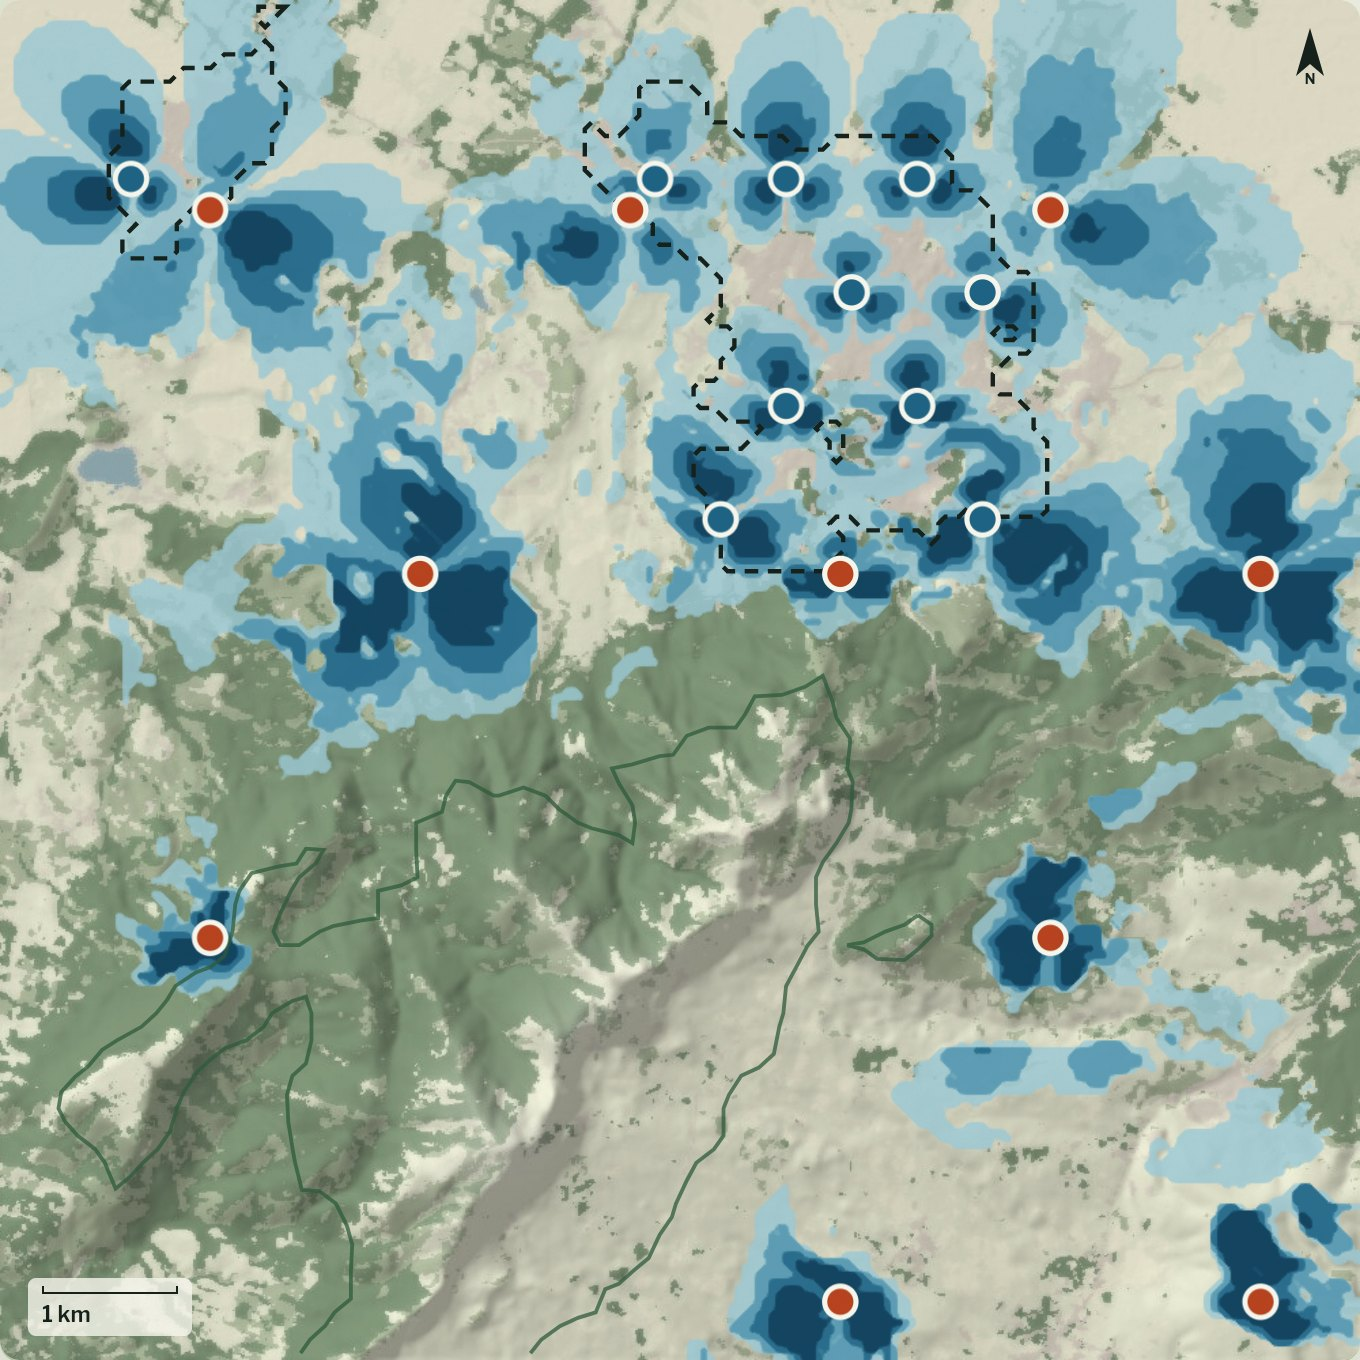
\includegraphics[width=0.56\textwidth]{cinr-mc1000.jpg}
\caption{C/(I+N) en DL avec les charges simulées.}
\label{fig-cinr-mc}
\end{figure}

Avec les charges de la simulation à \num{1000} utilisateurs (\cref{fig-cinr-mc}), la ville passe en grande partie au-dessus de \SI{-1}{\deci\bel}. Le \cref{tab-charge} compare les deux hypothèses sur le même réseau, avec les mêmes tilts.

\begin{table}[H]
\centering
\caption{Effet de la charge sur la qualité et les débits.}
\label{tab-charge}
\begin{tabular}{@{}lccc@{}}
\toprule
\thead{Indicateur} & \thead{Charge \SI{100}{\percent}} & \thead{Charge simulée} & \thead{Évolution} \\
\midrule
Surface C/(I+N) $\geq \SI{-1}{\deci\bel}$ & \SI{14,6}{\kilo\metre\squared} & \SI{36,1}{\kilo\metre\squared} & × 2,5 \\
C/(I+N) moyen & \SI{5,1}{\deci\bel} & \SI{6,6}{\deci\bel} & +\SI{1,5}{\deci\bel} \\
Débit DL moyen (zone servie) & \SI{18,7}{\Mbps} & \SI{34,0}{\Mbps} & \\
\bottomrule
\end{tabular}
\end{table}

En réutilisation~1, l'interférence reçue est proportionnelle à la charge des cellules voisines : passer de \SI{100}{\percent} à moins de \SI{20}{\percent} multiplie par 2,5 la surface utilisable en DL. Par zone, avec la charge simulée, la ville atteint \SI{99,5}{\percent} en UL ($\geq \SI{128}{\kbps}$) mais seulement \SI{78,9}{\percent} en DL ($\geq \SI{1}{\Mbps}$) ; la campagne atteint \SI{55,8}{\percent} en UL et \SI{38,0}{\percent} en DL.

\begin{retenir}
Il reste deux problèmes distincts : l'interférence entre sites urbains, qui limite le DL en ville, et la couverture derrière le massif, sur laquelle la charge n'a aucun effet.
\end{retenir}

\chapter{Simulations Monte-Carlo}
\label{ch-mc}

Une prédiction décrit le réseau en chaque point, pour une charge fixée à l'avance. Une simulation Monte-Carlo place de vrais utilisateurs : Atoll les tire au hasard selon la carte de trafic, calcule pour chacun son serveur, son SINR, son bearer et son débit, ainsi que la charge de chaque cellule, puis répète le tirage pour obtenir des statistiques. Le sujet demande des simulations pour 10, 100 et \num{1000} utilisateurs et leur fonction de distribution cumulative inverse (DCFI) sur un même graphique.

\section{Paramétrage}

\begin{itemize}
  \item \textbf{Nombre d'utilisateurs :} la carte de trafic contient \num{25359} utilisateurs potentiels (un par habitant). Le facteur d'échelle global de chaque groupe vaut $N / \num{25359}$, soit \SI{0,0394}{\percent}, \SI{0,394}{\percent} et \SI{3,94}{\percent} pour 10, 100 et \num{1000} utilisateurs. Les trois groupes partagent ainsi la même carte : leurs courbes sont comparables.
  \item \textbf{Répétitions :} 20 simulations par groupe ; charge maximale de \SI{80}{\percent} en DL et en UL ; paramètres de convergence par défaut.
  \item \textbf{Graine du générateur :} fixée à 1, ce qui rend les tirages reproductibles. Cette propriété sert au \cref{ch-opt} : les mêmes utilisateurs sont tirés sur le réseau initial et sur le réseau final.
\end{itemize}

Un utilisateur actif du service High Speed Internet demande environ \SI{1}{\Mbps} ; la demande de l'heure chargée calculée à l'Étape 1 (\SI{225}{\Mbps} en ville) correspond donc à quelques centaines d'utilisateurs simultanés. 10 utilisateurs représentent donc un réseau presque vide, 100 une charge normale et \num{1000} un test de stress au-delà de l'heure chargée.

\section{Résultats par groupe}

\begin{table}[H]
\centering
\caption{Résultats Monte-Carlo (moyenne de 20 tirages).}
\label{tab-mc}
\begin{tabular}{@{}lccc@{}}
\toprule
\thead{Indicateur} & \thead{MC-10} & \thead{MC-100} & \thead{MC-1000} \\
\midrule
Utilisateurs tirés (écart-type) & 9,95 (3,0) & 100 (11,3) & \num{1001,6} (35,6) \\
Rejetés & \SI{8,5}{\percent} & \SI{9,5}{\percent} & \SI{10,8}{\percent} \\
\quad dont pas de couverture / pas de service & 0,30 / 0,55 & 2,35 / 7,2 & 26,6 / 81,7 \\
\quad dont saturation & 0 & 0 & 0 \\
Demande DL & \SI{6,06}{\Mbps} & \SI{64,4}{\Mbps} & \SI{650,9}{\Mbps} \\
Débit DL servi (applicatif, cumulé) & \SI{4,23}{\Mbps} & \SI{40,2}{\Mbps} & \SI{257,3}{\Mbps} \\
Débit UL servi (applicatif, cumulé) & \SI{0,68}{\Mbps} & \SI{6,85}{\Mbps} & \SI{68,3}{\Mbps} \\
\bottomrule
\end{tabular}
\end{table}

Le nombre d'utilisateurs tirés varie autour de la demande : pour MC-10, la moyenne vaut 9,95 et l'écart-type 3,04, proche de $\sqrt{10} \approx 3{,}16$, ce qui correspond à un tirage de Poisson. Pour la demande DL de MC-10, le mélange de services donne $0{,}60 × 1024 + 0{,}25 × 128 + 0{,}15 × 12{,}2 \approx \SI{648}{\kbps}$ par utilisateur, soit environ \SI{6,4}{\Mbps} pour 9,95 utilisateurs, du même ordre que les \SI{6,06}{\Mbps} d'Atoll.

\section{Pourquoi des utilisateurs sont rejetés}
\label{sec-tests}

Atoll fait passer à chaque utilisateur tiré trois tests successifs ; la fenêtre de statistiques d'Atoll (\cref{fig-mc}b) donne le nombre d'échecs à chacun :
\begin{enumerate}
  \item Le signal arrive-t-il ? Au moins une cellule doit être reçue au-dessus du seuil de réception. Sinon : \enquote{pas de couverture}.
  \item Le signal est-il assez propre ? Le C/(I+N) doit atteindre le seuil du bearer le plus robuste, \SI{-1}{\deci\bel}. Sinon : \enquote{pas de service}. Ce seuil se lit dans les données exportées : tous les utilisateurs connectés ont un C/(I+N) d'au moins \SI{-0,9}{\deci\bel}, tous les \enquote{pas de service} au plus \SI{-1,1}{\deci\bel}.
  \item La cellule a-t-elle de la place ? Il doit rester des ressources radio (charge maximale de \SI{80}{\percent}). Sinon : saturation.
\end{enumerate}

\begin{figure}[H]
\centering
\begin{subfigure}[b]{0.56\textwidth}\centering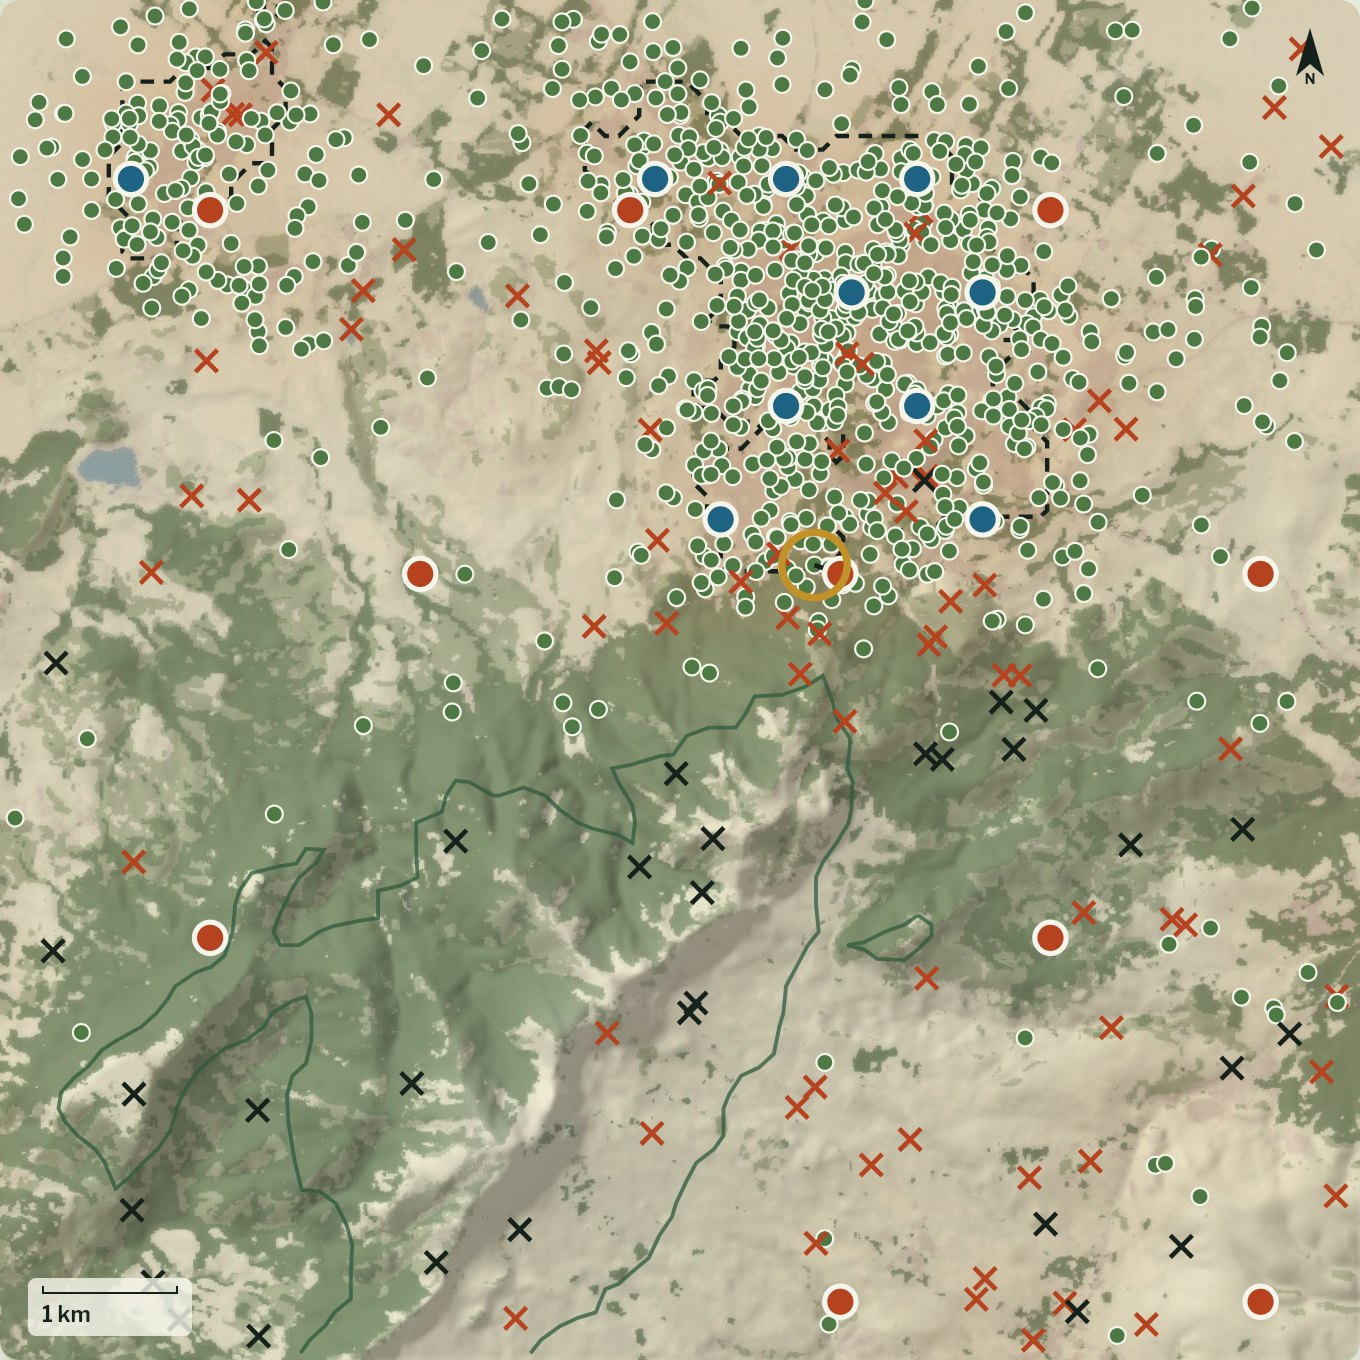
\includegraphics[width=\textwidth]{mc-tests.jpg}\caption{Un tirage de MC-1000.}\end{subfigure}\hfill
\begin{subfigure}[b]{0.42\textwidth}\centering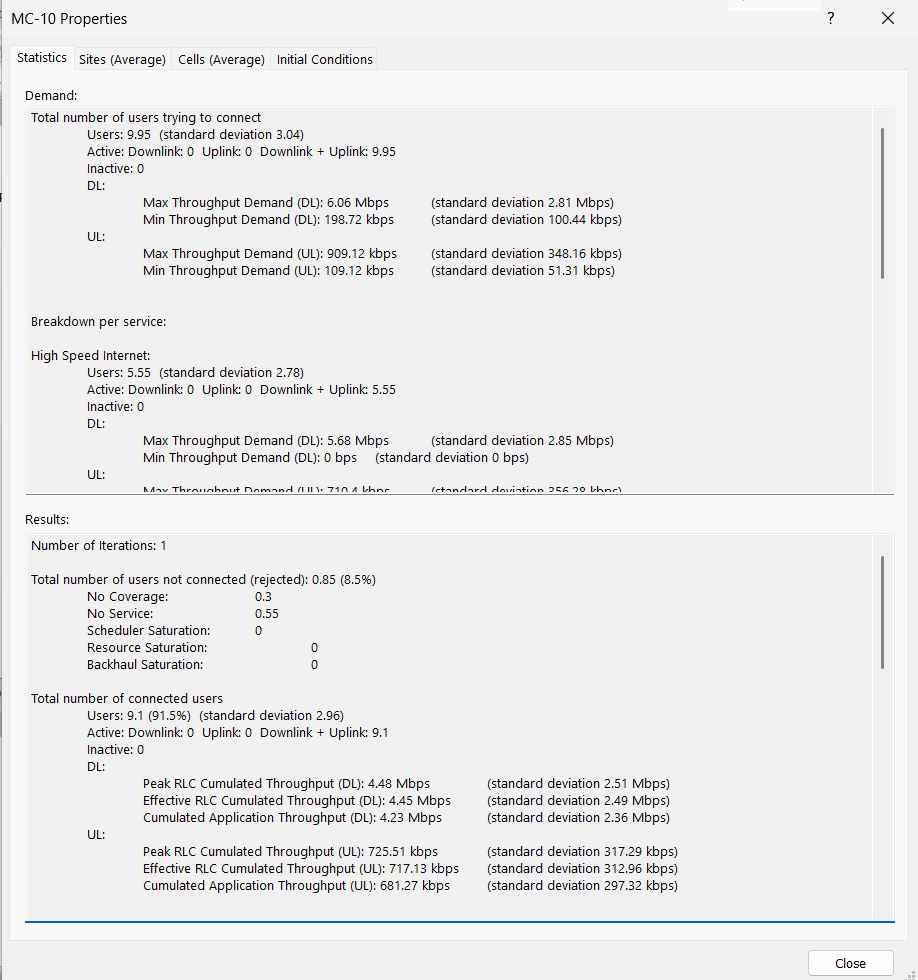
\includegraphics[width=\textwidth]{S04-05_MC10_statistiques.png}\caption{Statistiques d'Atoll (MC-10).}\end{subfigure}
\caption{Utilisateurs simulés et causes de rejet.}
\label{fig-mc}
\end{figure}

Sur la \cref{fig-mc}a, les utilisateurs connectés sont en vert, les \enquote{pas de couverture} en croix noires et les \enquote{pas de service} en croix rouges ; les sites urbains et ruraux sont en bleu et en terre cuite. Dans ce tirage de \num{1041} utilisateurs, 31 échouent au test 1, 77 au test 2 et \textbf{aucun au test 3} ; 933 sont connectés. Sur les 20 tirages, le taux de saturation est nul pour les trois groupes. Tous les rejets viennent donc du signal (couverture et interférence), aucun de la capacité. Les 108 rejetés se répartissent en 76 dans la campagne loin des sites, 14 sur le massif et 18 en ville, dont 17 à l'intérieur des bâtiments, où \SI{15}{\deci\bel} de pénétration s'ajoutent à l'interférence entre sites urbains.

\section{La DCFI}
\label{sec-dcfi}

La DCFI est la fonction de distribution cumulative inverse (ou complémentaire) du débit : pour chaque débit $x$, elle donne la proportion des utilisateurs qui obtiennent au moins $x$,
\begin{equation}
  \text{DCFI}(x) = P(\text{débit} \geq x) = 1 - F(x),
\end{equation}
où $F$ est la fonction de répartition. Pour un débit choisi sur l'axe horizontal, la courbe donne la part des utilisateurs servis au moins à ce débit. Nous l'avons tracée à partir du débit applicatif de \emph{chaque} utilisateur, exporté d'Atoll (onglet \enquote{Mobiles} des simulations), en comptant les utilisateurs rejetés à \SI{0}{\kbps}. Les courbes portent sur les utilisateurs du service High Speed Internet, celui qui porte l'objectif de bord de cellule.

Échantillons utilisés : MC-10, les 20 tirages (199 utilisateurs, dont 111 HSI) ; MC-100, 5 tirages (528, dont 326 HSI) ; MC-1000, 2 tirages (\num{2104}, dont \num{1224} HSI). Leur taux de rejet (\SI{8,5}{\percent}, \SI{9,3}{\percent}, \SI{10,5}{\percent}) est proche de la moyenne des 20 tirages : les échantillons sont représentatifs.

\begin{figure}[H]
\centering
\begin{subfigure}[b]{0.49\textwidth}\centering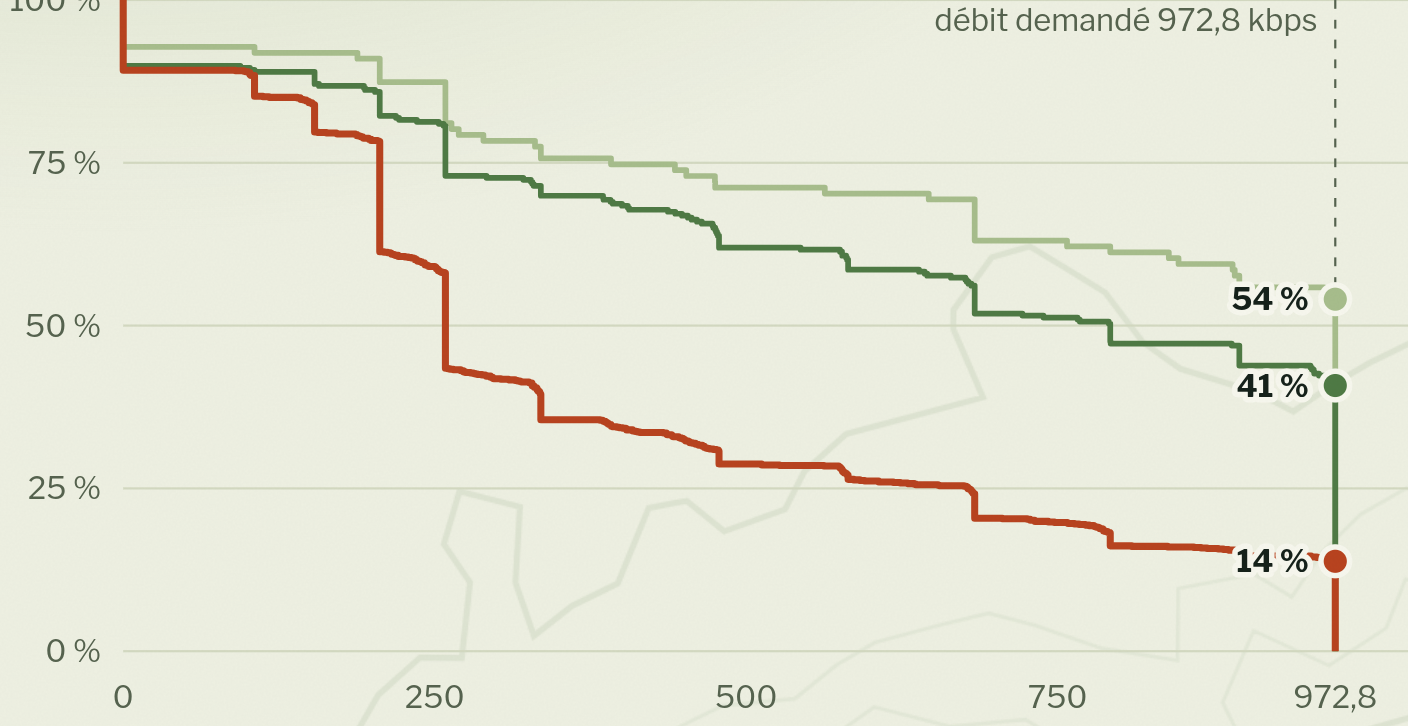
\includegraphics[width=\textwidth]{dcfi-dl.png}\caption{DL.}\end{subfigure}\hfill
\begin{subfigure}[b]{0.49\textwidth}\centering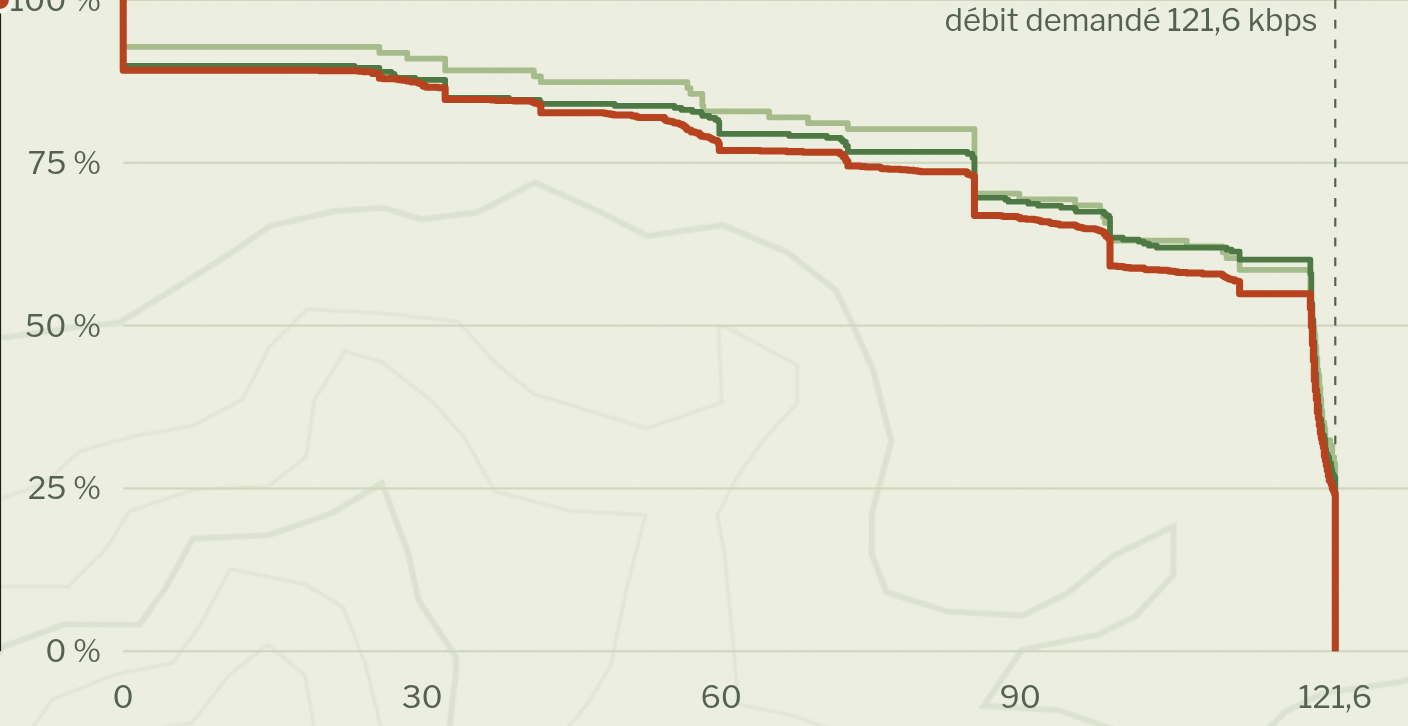
\includegraphics[width=\textwidth]{dcfi-ul.png}\caption{UL.}\end{subfigure}
\caption{DCFI du débit applicatif des utilisateurs HSI.}
\label{fig-dcfi}
\end{figure}

Sur la \cref{fig-dcfi}, les courbes de 10, 100 et \num{1000} utilisateurs sont en vert clair, en vert et en terre cuite. Le débit demandé vaut \SI{972,8}{\kbps} en DL et \SI{121,6}{\kbps} en UL : ce sont les débits applicatifs $1024 × 0{,}95$ et $128 × 0{,}95$.

\begin{table}[H]
\centering
\caption{Lecture des DCFI (utilisateurs HSI).}
\label{tab-dcfi}
\begin{tabular}{@{}lccc@{}}
\toprule
\thead{Indicateur} & \thead{MC-10} & \thead{MC-100} & \thead{MC-1000} \\
\midrule
Part au débit demandé en DL & \SI{54}{\percent} & \SI{41}{\percent} & \textcolor{terre}{\textbf{\SI{14}{\percent}}} \\
Débit DL médian & \SI{973}{\kbps} & \SI{792}{\kbps} & \textcolor{terre}{\textbf{\SI{259}{\kbps}}} \\
Part au débit demandé en UL & \SI{32}{\percent} & \SI{29}{\percent} & \SI{26}{\percent} \\
Tous services : part servie au débit demandé en DL & \SI{59}{\percent} & \SI{47}{\percent} & \SI{25}{\percent} \\
\bottomrule
\end{tabular}
\end{table}

\section{Synthèse et impact sur le dimensionnement}
\label{sec-p4}

Les courbes se lisent en trois points.
\begin{enumerate}
  \item À $x = 0$, les trois courbes partent d'environ \SI{90}{\percent} : environ \SI{10}{\percent} des utilisateurs sont rejetés quel que soit leur nombre, tous pour une raison de signal. Ce problème de couverture est la cible de l'optimisation.
  \item Le débit DL médian passe de 973 à \SI{259}{\kbps} de 10 à \num{1000} utilisateurs. Le service est \enquote{best effort} : faute de place, Atoll donne moins de débit à l'utilisateur au lieu de le rejeter. Le DL est donc limité par la capacité et l'interférence.
  \item Les trois courbes UL sont presque superposées. L'UL est limité par la puissance du terminal, comme l'annonçait le bilan de liaison (liaison montante limitante de \SI{2}{\deci\bel}).
\end{enumerate}

Ces résultats confirment l'Étape 1 sur deux points : la liaison montante limite la couverture, et la capacité n'est pas le facteur dimensionnant aujourd'hui (aucune saturation, même à \num{1000} utilisateurs). Ils précisent aussi la limite de capacité : à \num{1000} utilisateurs simultanés, la médiane tombe à \SI{259}{\kbps}. L'objectif de \SI{1}{\Mbps} tient pour quelques centaines d'utilisateurs simultanés, ce qui couvre la demande actuelle de l'heure chargée ; au-delà, il faudra ajouter de la capacité (une seconde porteuse ou de petites cellules) et non de la couverture.

Un résultat reste inexpliqué : même dans MC-10, \SI{46}{\percent} des utilisateurs HSI reçoivent moins de \SI{1}{\Mbps} alors qu'ils sont seuls dans leur cellule avec un bon C/I (médiane d'environ \SI{20}{\deci\bel}). Ce n'est expliqué ni par la mobilité ni par le nombre d'utilisateurs par cellule ; il s'agit probablement d'une règle interne de l'ordonnanceur d'Atoll, que nous n'avons pas pu vérifier. Nous la signalons parmi les limites (\cref{sec-limites}).

\chapter{Optimisation}
\label{ch-opt}

\section{Méthode}

Les actions sont appliquées une à la fois. Après chaque action, les prédictions sont recalculées et notre script mesure la couverture par zone sur les rasters exportés, de la même façon pour toutes les actions. L'action est gardée si elle améliore les objectifs sans dégrader le reste, et annulée sinon. Les mesures avant et après sont ainsi comparables d'une action à l'autre. Cette boucle reprend celle du cours : prédictions de couverture et d'interférence, ajustement, puis densification~\cite{afif2026cours}.

\section{Diagnostic}

Après les deux premières actions, il reste \SI{13,0}{\kilo\metre\squared} de trous ruraux en outdoor. Pour atteindre \SI{95}{\percent} des \SI{76,95}{\kilo\metre\squared} ruraux, au plus \SI{3,85}{\kilo\metre\squared} peuvent rester découverts : il faut regagner environ \SI{9}{\kilo\metre\squared}.

\begin{figure}[H]
\centering
\begin{minipage}[c]{0.44\textwidth}\centering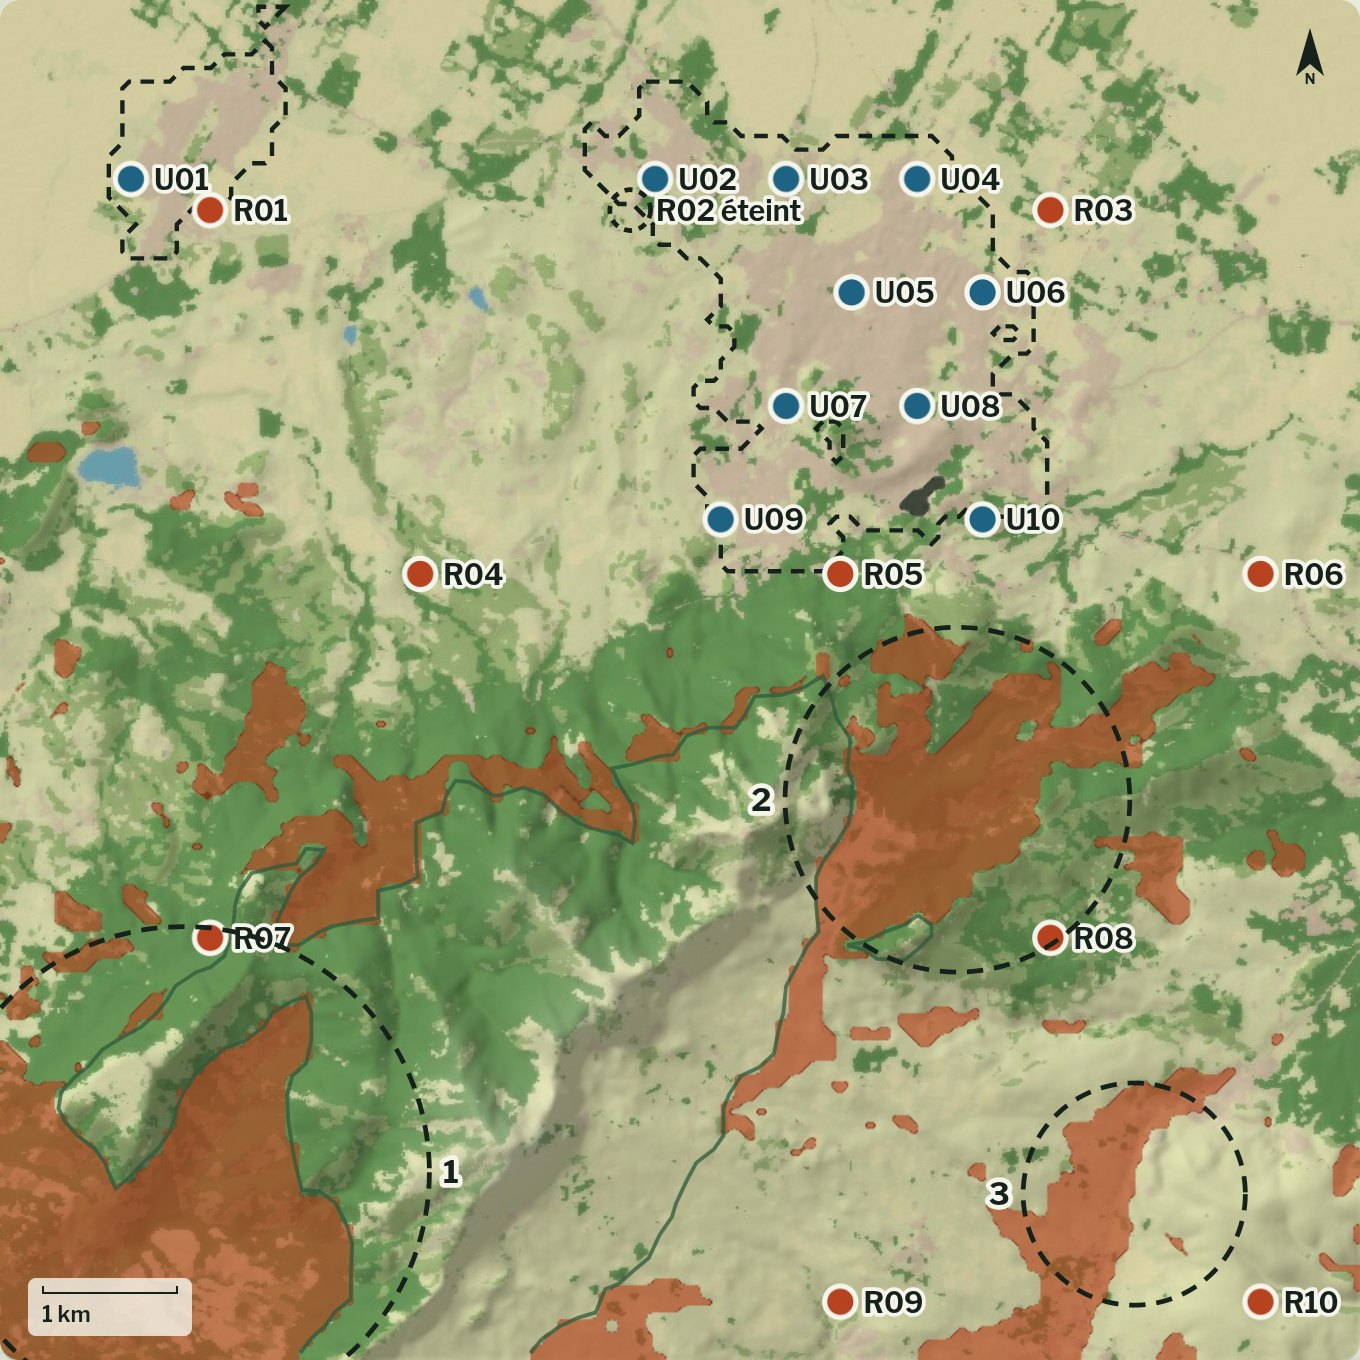
\includegraphics[width=\textwidth]{diagnostic.jpg}\end{minipage}\hfill
\begin{minipage}[c]{0.52\textwidth}
\captionof{table}{Trous ruraux (raster d'Atoll).}
\label{tab-trous}
\footnotesize
\begin{tabular}{@{}lrr@{}}
\toprule
\thead{Trou} & \thead{Surface} & \thead{Habitants} \\
\midrule
1 · coin sud-ouest & \SI{4,84}{\kilo\metre\squared} & 128 \\
2 · pied est de la crête & \SI{3,25}{\kilo\metre\squared} & 144 \\
3 · sud-est & \SI{1,81}{\kilo\metre\squared} & 198 \\
poches ouest et nord-ouest & \SI{2,09}{\kilo\metre\squared} & 52 \\
\midrule
total, avec les pixels isolés & \SI{13,0}{\kilo\metre\squared} & \\
\bottomrule
\end{tabular}
\end{minipage}
\captionof{figure}{Trous ruraux avant les actions de couverture.}
\label{fig-diag}
\end{figure}

En ville, la couverture est atteinte ; le problème est l'interférence (\cref{sec-cinr}), due à trop de recouvrement et à un tilt trop faible. Les actions 1, 2 et 7 visent la ville, les actions 3 à 6 la campagne.

\section{Action 1 : tilt urbain de 4° à 6°}

Le diagramme vertical de l'antenne, relevé dans Atoll, a une ouverture d'environ \ang{6,3} à \SI{-3}{\deci\bel} et n'est atténué que de \SI{4,1}{\deci\bel} à l'horizon. Avec un tilt de \ang{4}, le bord supérieur du lobe (\ang{3,4} au-dessus de l'axe) n'est incliné que de \ang{0,6} et touche le sol à $30 / \tan 0{,}6^\circ \approx \SI{2,9}{\kilo\metre}$, cinq fois le rayon de la cellule : chaque secteur arrose ses voisins. Le tilt qui place ce bord au bord de la cellule vaut
\begin{equation}
  \arctan\!\left(\frac{30}{640}\right) + 3{,}4^\circ \approx 2{,}7^\circ + 3{,}4^\circ \approx 6{,}1^\circ .
\end{equation}
Nous avons ajouté \ang{2} de tilt mécanique aux \ang{4} électriques des secteurs urbains. La \cref{fig-tilt} montre l'effet : avec \ang{6}, le bord du lobe touche le sol à \SI{0,66}{\kilo\metre}, au bord de la cellule.

\begin{figure}[H]
\centering
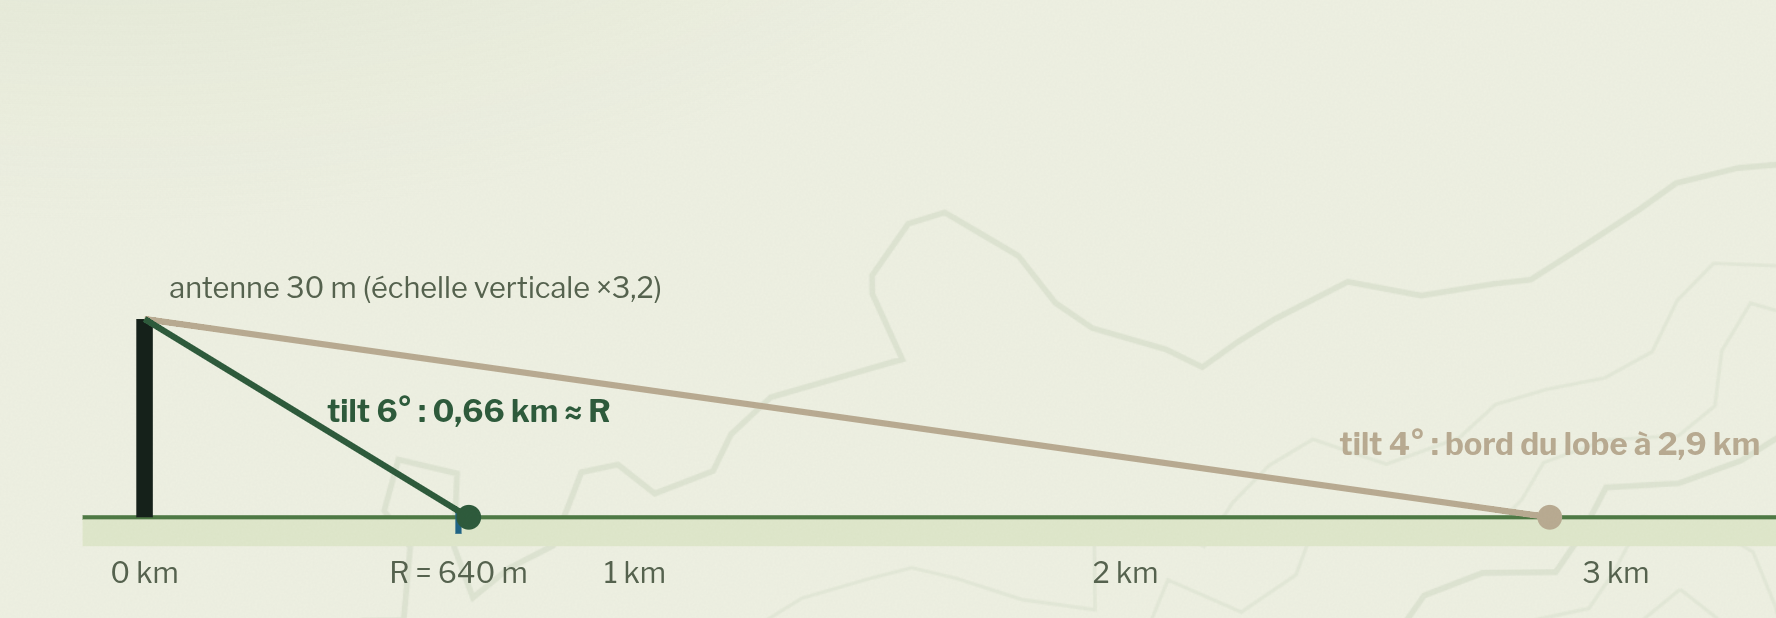
\includegraphics[width=0.8\textwidth]{tilt.png}
\caption{Géométrie du tilt urbain (échelle verticale × 3,2).}
\label{fig-tilt}
\end{figure}

\begin{table}[H]
\centering
\caption{Action 1 : tilt urbain de \ang{4} à \ang{6}.}
\label{tab-a1}
\begin{tabular}{@{}lccc@{}}
\toprule
\thead{Indicateur} & \thead{Avant} & \thead{Après} & \thead{Évolution} \\
\midrule
Surface à 4 serveurs ou plus & \SI{2,39}{\kilo\metre\squared} & \SI{1,45}{\kilo\metre\squared} & $-\SI{39}{\percent}$ \\
Surface C/(I+N) $\geq \SI{-1}{\deci\bel}$ & \SI{13,1}{\kilo\metre\squared} & \SI{14,6}{\kilo\metre\squared} & $+\SI{11}{\percent}$ \\
Couverture urbaine indoor & \SI{99,5}{\percent} & \SI{99,4}{\percent} & $-0{,}1$ pt \\
Couverture rurale outdoor & \SI{83,4}{\percent} & \SI{83,2}{\percent} & sites ruraux inchangés \\
\bottomrule
\end{tabular}
\end{table}

\begin{verdict}
Action \gardee{} (mesures à charge \SI{100}{\percent}) : le recouvrement à quatre serveurs baisse de \SI{39}{\percent} et la surface de bonne qualité augmente de \SI{11}{\percent}, pour une perte de couverture urbaine négligeable.
\end{verdict}

\section{Action 2 : désactivation du site R02}

R02, site rural de la grille nominale, se trouve à \SI{300}{\metre} du site urbain U02. Il a été désactivé plutôt que supprimé, car Atoll efface toutes les simulations qui utilisent un site supprimé. Les mesures du \cref{tab-a2} utilisent les charges simulées à \num{1000} utilisateurs.

\begin{table}[H]
\centering
\caption{Action 2 : désactivation de R02.}
\label{tab-a2}
\begin{tabular}{@{}lccc@{}}
\toprule
\thead{Indicateur} & \thead{Avant} & \thead{Après} & \thead{Évolution} \\
\midrule
Couverture urbaine indoor & \SI{99,4}{\percent} & \SI{99,4}{\percent} & 0 \\
Couverture rurale outdoor & \SI{83,2}{\percent} & \SI{83,1}{\percent} & $-0{,}1$ pt \\
Surface à 2 serveurs ou plus & \SI{24,37}{\kilo\metre\squared} & \SI{23,10}{\kilo\metre\squared} & $-\SI{5}{\percent}$ \\
Surface C/(I+N) $\geq \SI{-1}{\deci\bel}$ & \SI{36,13}{\kilo\metre\squared} & \SI{36,82}{\kilo\metre\squared} & $+\SI{2}{\percent}$ \\
Nombre de sites & 20 & 19 & $-1$ \\
\bottomrule
\end{tabular}
\end{table}

\begin{verdict}
Action \gardee{} : le gain radio est faible, mais un site entier est économisé (pylône, équipements, énergie, loyer) sans perte de couverture. R01, également proche d'un site urbain, a été conservé : la simulation montre que sa cellule R01\_1 est la plus chargée du réseau, car elle sert le village du nord-ouest.
\end{verdict}

\section{Actions 3 et 3b : déplacer ou réorienter R07, rejetées}

R07 est placé sur le flanc du massif, à \SI{503}{\metre}. Première idée (action 3) : le déplacer au centre du trou sud-ouest, à \SI{391}{\metre}. Seconde idée (action 3b) : le laisser en place et tourner ses secteurs vers le coin (azimuts \ang{30}, \ang{190}, \ang{290}).

\begin{table}[H]
\centering
\caption{Actions 3 et 3b, mesurées puis annulées.}
\label{tab-a3}
\small\setlength{\tabcolsep}{5pt}
\begin{tabular}{@{}lccl@{}}
\toprule
\thead{Action} & \thead{Rural\\outdoor (surface)} & \thead{Rural\\(population)} & \thead{Verdict} \\
\midrule
Avant (R02 désactivé) & \SI{83,1}{\percent} & \SI{95,2}{\percent} & \\
3 · R07 déplacé dans le coin sud-ouest & \SI{82,7}{\percent} & \SI{94,7}{\percent} & \rejetee \\
3b · R07 réorienté (\ang{30}/\ang{190}/\ang{290}) & \SI{82,4}{\percent} & \SI{95,1}{\percent} & \rejetee \\
\bottomrule
\end{tabular}
\end{table}

Déplacé, R07 couvre le coin mais ne voit plus la plaine ouest qu'il servait depuis sa hauteur. Réorienté, il ne gagne que \SI{0,01}{\kilo\metre\squared} dans le coin (comparaison pixel à pixel). Le profil du terrain explique ces deux échecs (\cref{fig-profil}). R07 est à \SI{503}{\metre}, plus \SI{30}{\metre} de mât, et le coin sud-ouest à \SI{389}{\metre}, à \SI{2,4}{\kilo\metre} ; entre les deux, la crête monte à \SI{807}{\metre} et coupe la ligne de vue. Changer l'azimut ne sert à rien : seul un site placé dans le coin peut servir cette zone d'ombre.

\begin{figure}[H]
\centering
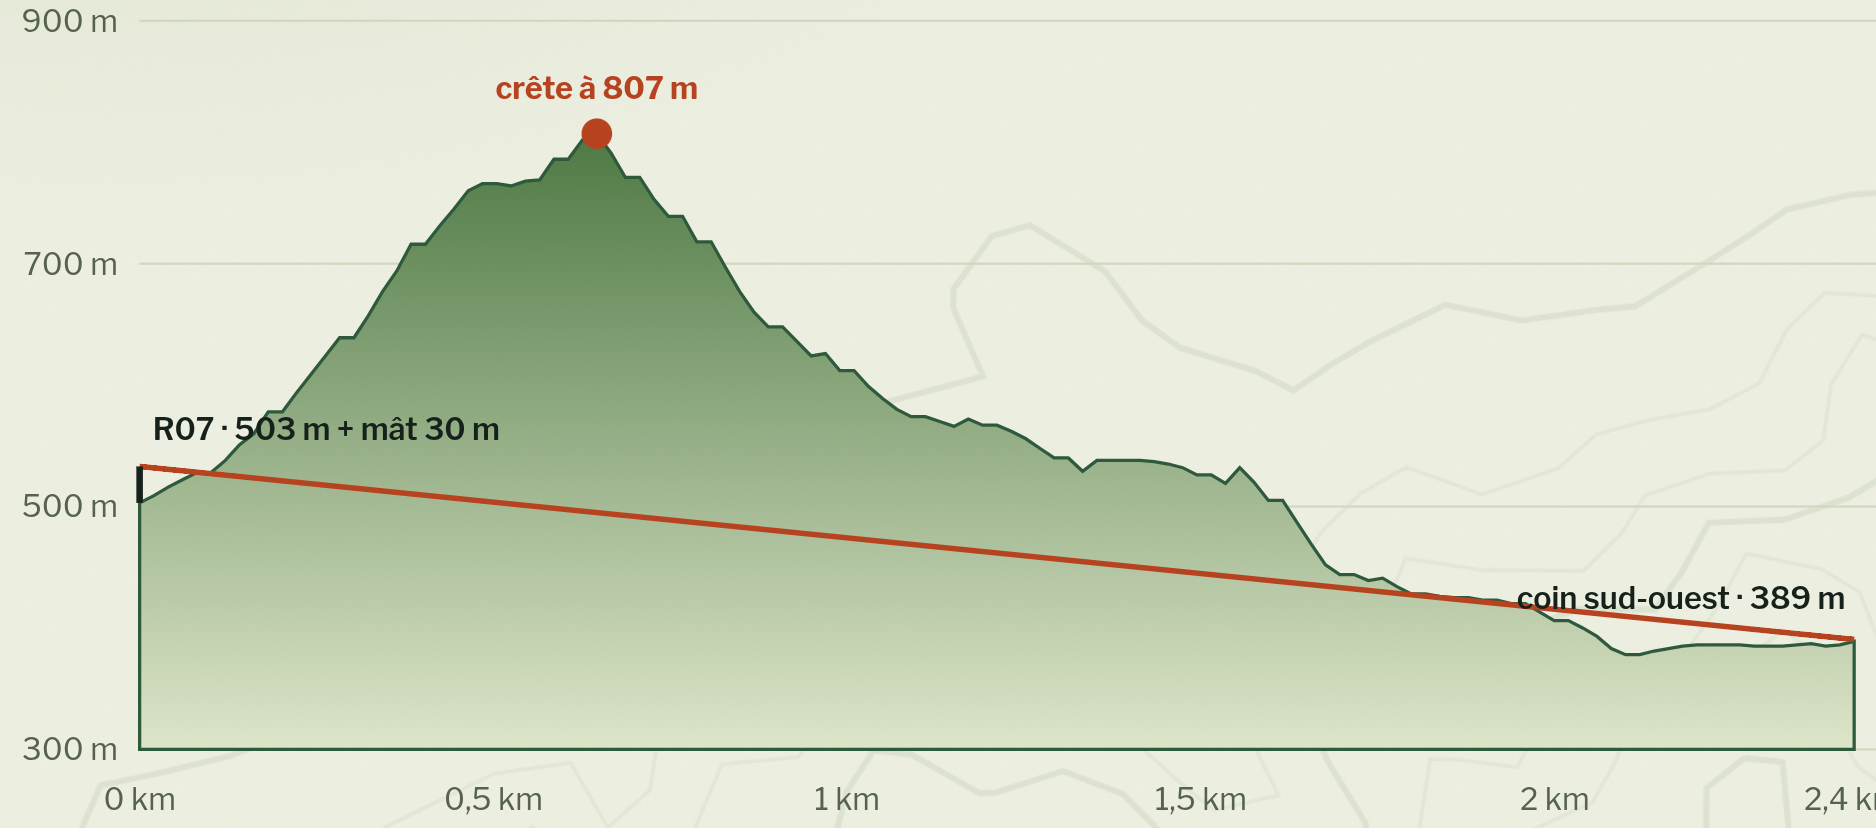
\includegraphics[width=0.85\textwidth]{profil-r07.png}
\caption{Profil du terrain entre R07 et le coin sud-ouest.}
\label{fig-profil}
\end{figure}

\section{Actions 4 et 5 : deux sites là où le relief l'exige}

Le budget de R02 est déplacé là où la couverture manque : un site R11 est créé au centre du trou sud-ouest (X = \SI{597240}{\metre}, Y = \SI{4023060}{\metre}, \SI{391}{\metre}), puis un site R12 au centre du trou du pied est (X = \SI{603230}{\metre}, Y = \SI{4026200}{\metre}).

\begin{table}[H]
\centering
\caption{Actions 4 et 5 : ajout des sites R11 et R12.}
\label{tab-a45}
\small\setlength{\tabcolsep}{5pt}
\begin{tabular}{@{}lccccl@{}}
\toprule
\thead{Étape} & \thead{Rural\\(surface)} & \thead{Rural\\(population)} & \thead{Urbain\\indoor} & \thead{Sites} & \thead{Verdict} \\
\midrule
Avant & \SI{83,1}{\percent} & \SI{95,2}{\percent} & \SI{99,4}{\percent} & 19 & \\
4 · + R11 (sud-ouest) & \SI{87,1}{\percent} & \SI{95,8}{\percent} & \SI{99,4}{\percent} & 20 & \gardee \\
5 · + R12 (pied est) & \SI{90,3}{\percent} & \SI{96,6}{\percent} & \SI{99,4}{\percent} & 21 & \gardee \\
\bottomrule
\end{tabular}
\end{table}

\begin{figure}[H]
\centering
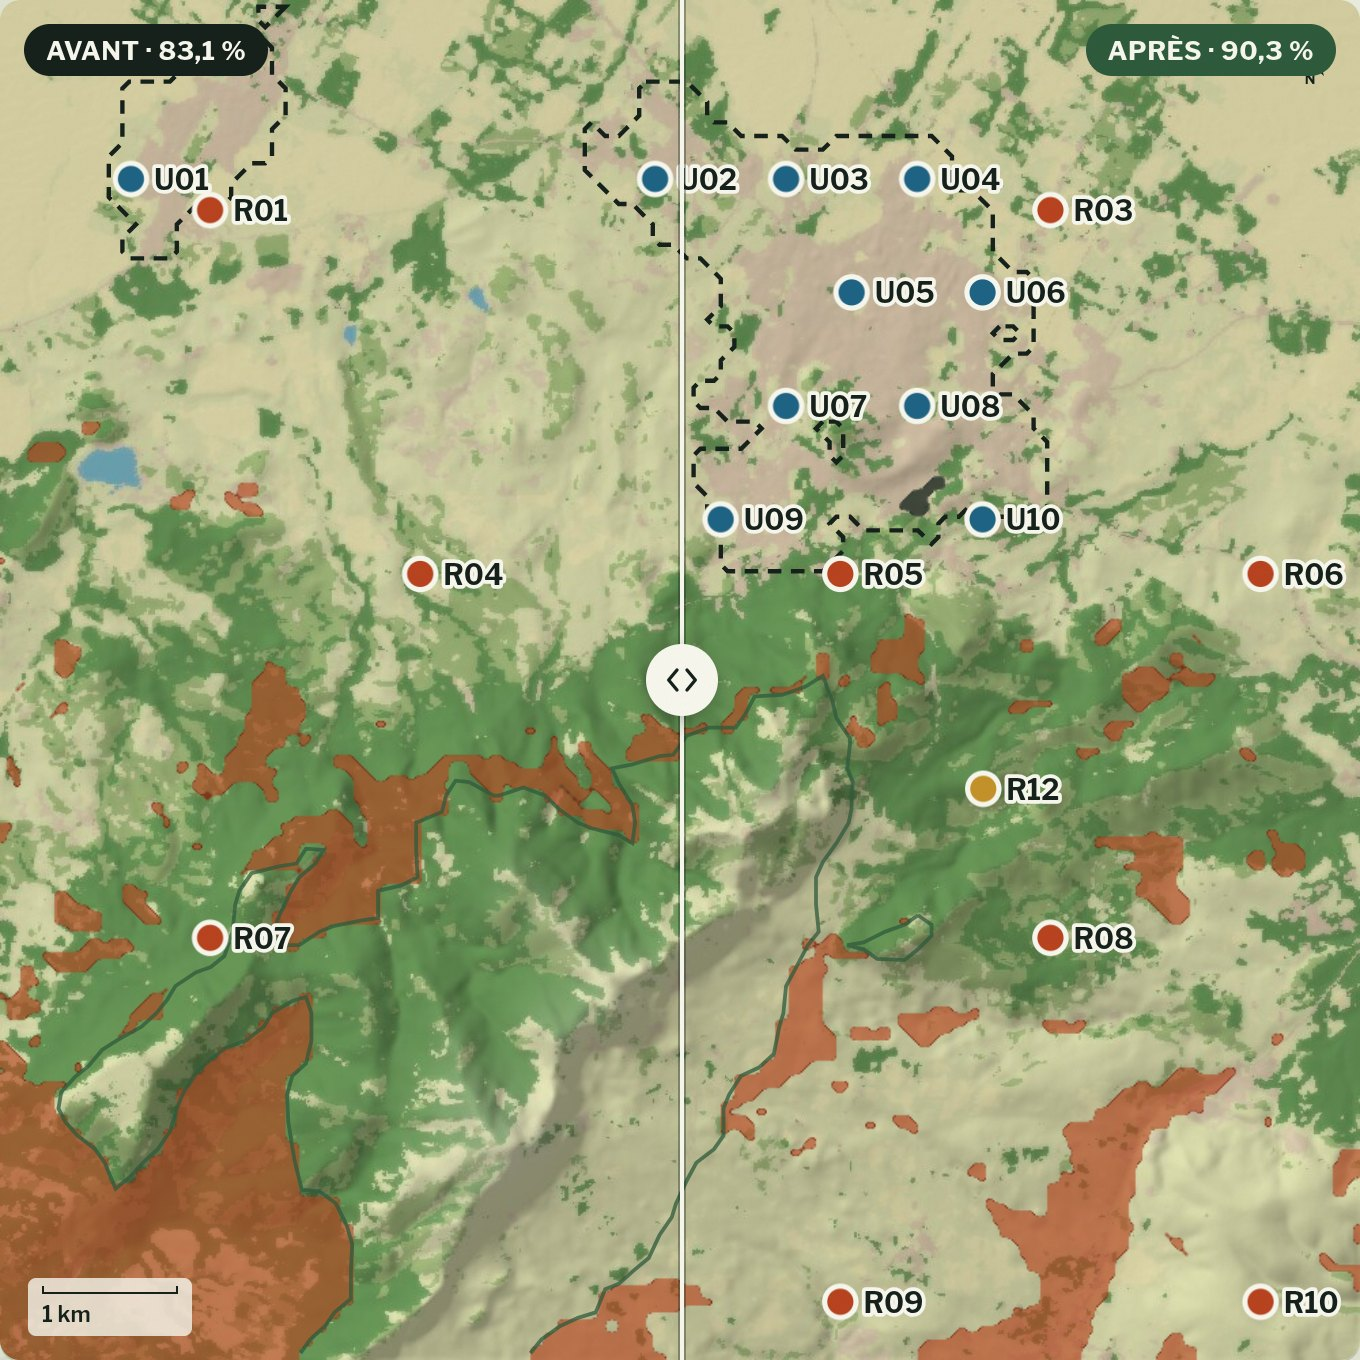
\includegraphics[width=0.58\textwidth]{r11-r12.jpg}
\caption{Couverture avant et après l'ajout de R11 et R12.}
\label{fig-r11r12}
\end{figure}

Sur la \cref{fig-r11r12}, la carte de gauche est le réseau sans R02, celle de droite le réseau avec R11 et R12 (en or) : les deux grands trous ruraux sont comblés.

Le réseau compte alors 21 sites, le nombre prévu par l'Étape 1, mais pas aux mêmes endroits. Nous n'ajoutons pas d'autre site. Il reste 4,7 points à gagner : le meilleur site suivant (au sud-est) apporterait environ 2,3 points, et il en faudrait encore environ trois pour atteindre \SI{95}{\percent} en surface, pour quelque 300 habitants dispersés, alors que \SI{96,6}{\percent} de la population rurale est déjà couverte. La suite est confiée au réglage automatique des antennes.

\section{Action 6 : planification automatique (ACP)}

Le module ACP (\emph{Automatic Cell Planning}) d'Atoll cherche la combinaison de réglages d'antennes qui maximise des objectifs de couverture. Nous lui avons donné nos objectifs : RSRP $\geq \SI{-120}{\dBm}$ sur \SI{95}{\percent} de la zone (son seuil par défaut était \SI{-105}{\dBm}) et RSRQ $\geq \SI{-15}{\deci\bel}$ sur \SI{85}{\percent}. Les réglages autorisés étaient le tilt électrique (\ang{0} à \ang{10}), l'azimut (± \ang{20}) et le tilt mécanique (\ang{0} à \ang{5}) ; la sélection de sites a été désactivée, car les sites sont décidés par nos actions mesurées. Le calcul (380 itérations) converge après environ 90 itérations.

\begin{figure}[H]
\centering
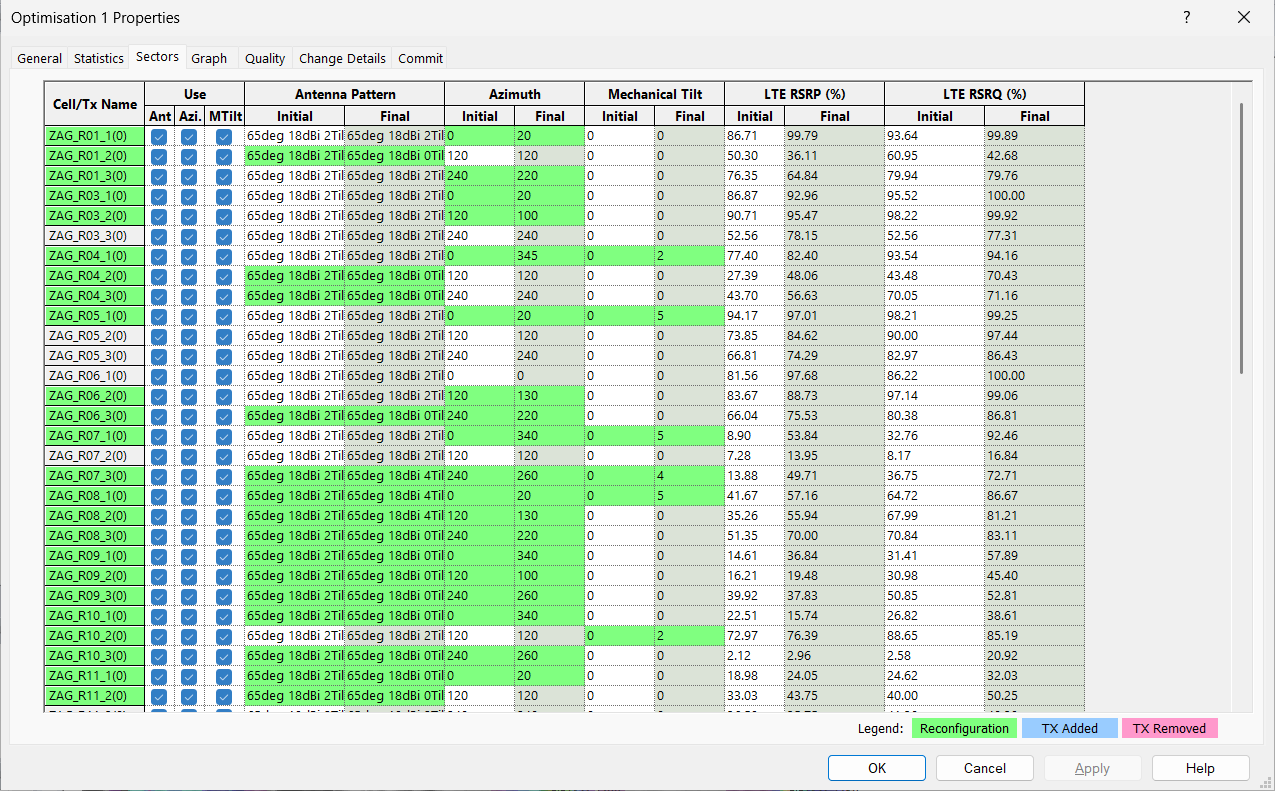
\includegraphics[width=0.75\textwidth]{acp_secteurs.png}
\caption{Changements proposés par l'ACP, secteur par secteur.}
\label{fig-acp}
\end{figure}

La \cref{fig-acp} détaille les propositions. L'ACP propose une soixantaine de changements, surtout sur les secteurs ruraux : beaucoup de tilts électriques ramenés de \ang{2} à \ang{0} pour porter plus loin, quelques secteurs basculés de \ang{2} à \ang{4}, des azimuts tournés jusqu'à \ang{20} et un tilt mécanique sur certains secteurs tournés vers la ville. Il relève aussi trois secteurs urbains de bordure orientés vers la campagne (U01\_3, U02\_3, U09\_3). Les premiers changements apportent l'essentiel du gain.

L'ACP évalue ses objectifs sur toute la zone de calcul d'Atoll (\SI{240}{\kilo\metre\squared}, en grande partie hors de nos cartes et loin des sites), d'où une couverture de départ de \SI{21,7}{\percent} selon sa propre mesure. Nous n'utilisons donc que son gain \emph{relatif} (+4,3 points) et vérifions chaque proposition avec nos propres prédictions :

\begin{table}[H]
\centering
\caption{Action 6 : réglages de l'ACP.}
\label{tab-acp}
\begin{tabular}{@{}lccc@{}}
\toprule
\thead{Indicateur} & \thead{Avant ACP} & \thead{Après ACP} & \thead{Évolution} \\
\midrule
Couverture rurale outdoor (surface) & \SI{90,3}{\percent} & \textbf{\SI{94,3}{\percent}} & +4,0 pts \\
Couverture rurale outdoor (population) & \SI{96,6}{\percent} & \SI{97,9}{\percent} & +1,3 pt \\
Couverture urbaine indoor & \SI{99,4}{\percent} & \SI{99,7}{\percent} & +0,3 pt \\
\bottomrule
\end{tabular}
\end{table}

\begin{verdict}
Action \gardee{} : le gain mesuré sur notre zone (+4,0 points) correspond au gain annoncé par l'ACP sur la sienne (+4,3 points). Il reste 0,7 point (environ \SI{0,5}{\kilo\metre\squared}) pour atteindre \SI{95}{\percent}, moins que l'incertitude du modèle.
\end{verdict}

\section{Action 7 : tilt urbain à 8°, rejetée}

Pour réduire encore l'interférence urbaine, les secteurs urbains ont été basculés à \ang{8}. Le DL en ville gagne 1,2 point (de \SI{79,4}{\percent} à \SI{80,6}{\percent} de la surface à \SI{1}{\Mbps}), un écart dans le bruit du modèle, tandis que la campagne perd 0,1 point de couverture et 0,6 point de DL. L'action est \rejetee{} : le tilt de \ang{6} est déjà proche de l'optimum géométrique de \ang{6,1}.

\section{Action 8 : relations de voisinage (ANR)}

Le module ANR (\emph{Automatic Neighbour Relations}) construit les listes de voisins utilisées pour le handover. Il a été lancé avec une distance maximale de \SI{10}{\kilo\metre}, au plus 16 voisins par cellule, une marge de handover de \SI{0}{} à \SI{5}{\deci\bel} (la marge de notre carte de recouvrement) et des relations symétriques. Il attribue en général 3 à 6 voisins par cellule. L'ANR ne change pas les cartes radio ; il permet le handover entre les cellules qui se recouvrent, utile pour les utilisateurs mobiles. Après le tilt de \ang{6}, les cellules urbaines n'ont pas beaucoup plus de voisins que les cellules rurales, signe que le recouvrement a été contenu.

\section{Le réseau final}
\label{sec-final}

Le réseau final compte 21 sites : le réseau initial, sans R02, avec R11 et R12, le tilt urbain de \ang{6} et les réglages de l'ACP. Une nouvelle simulation à \num{1000} utilisateurs, avec la même graine, a fourni les charges finales, puis toutes les prédictions ont été recalculées.

\begin{figure}[H]
\centering
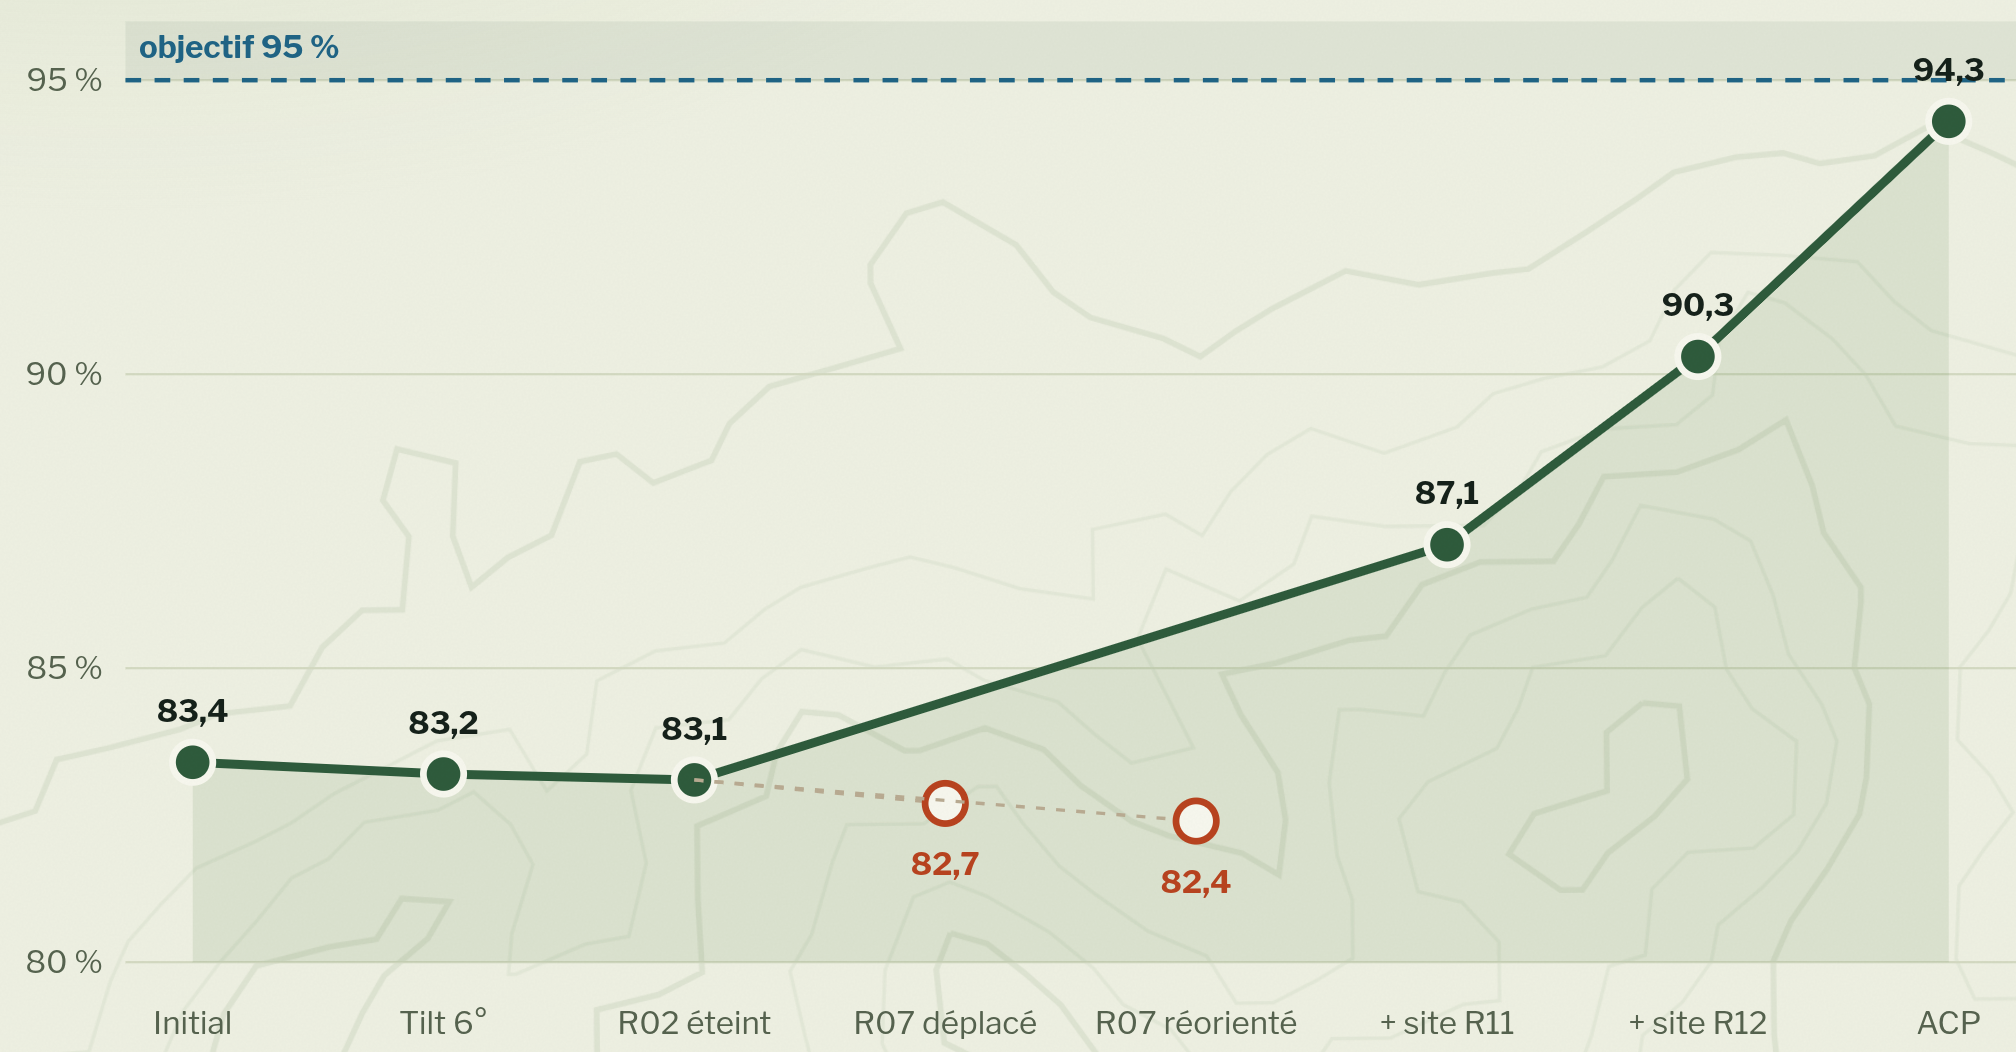
\includegraphics[width=0.9\textwidth]{progression.png}
\caption{Couverture rurale outdoor après chaque action.}
\label{fig-progression}
\end{figure}

Sur la \cref{fig-progression}, les cercles creux sont les actions rejetées, mesurées puis annulées ; la ligne pointillée est l'objectif de \SI{95}{\percent}. Sur la \cref{fig-ombre-final}, R11 et R12 (en or) sont posés à l'intérieur de l'ombre de la crête.

\begin{figure}[H]
\centering
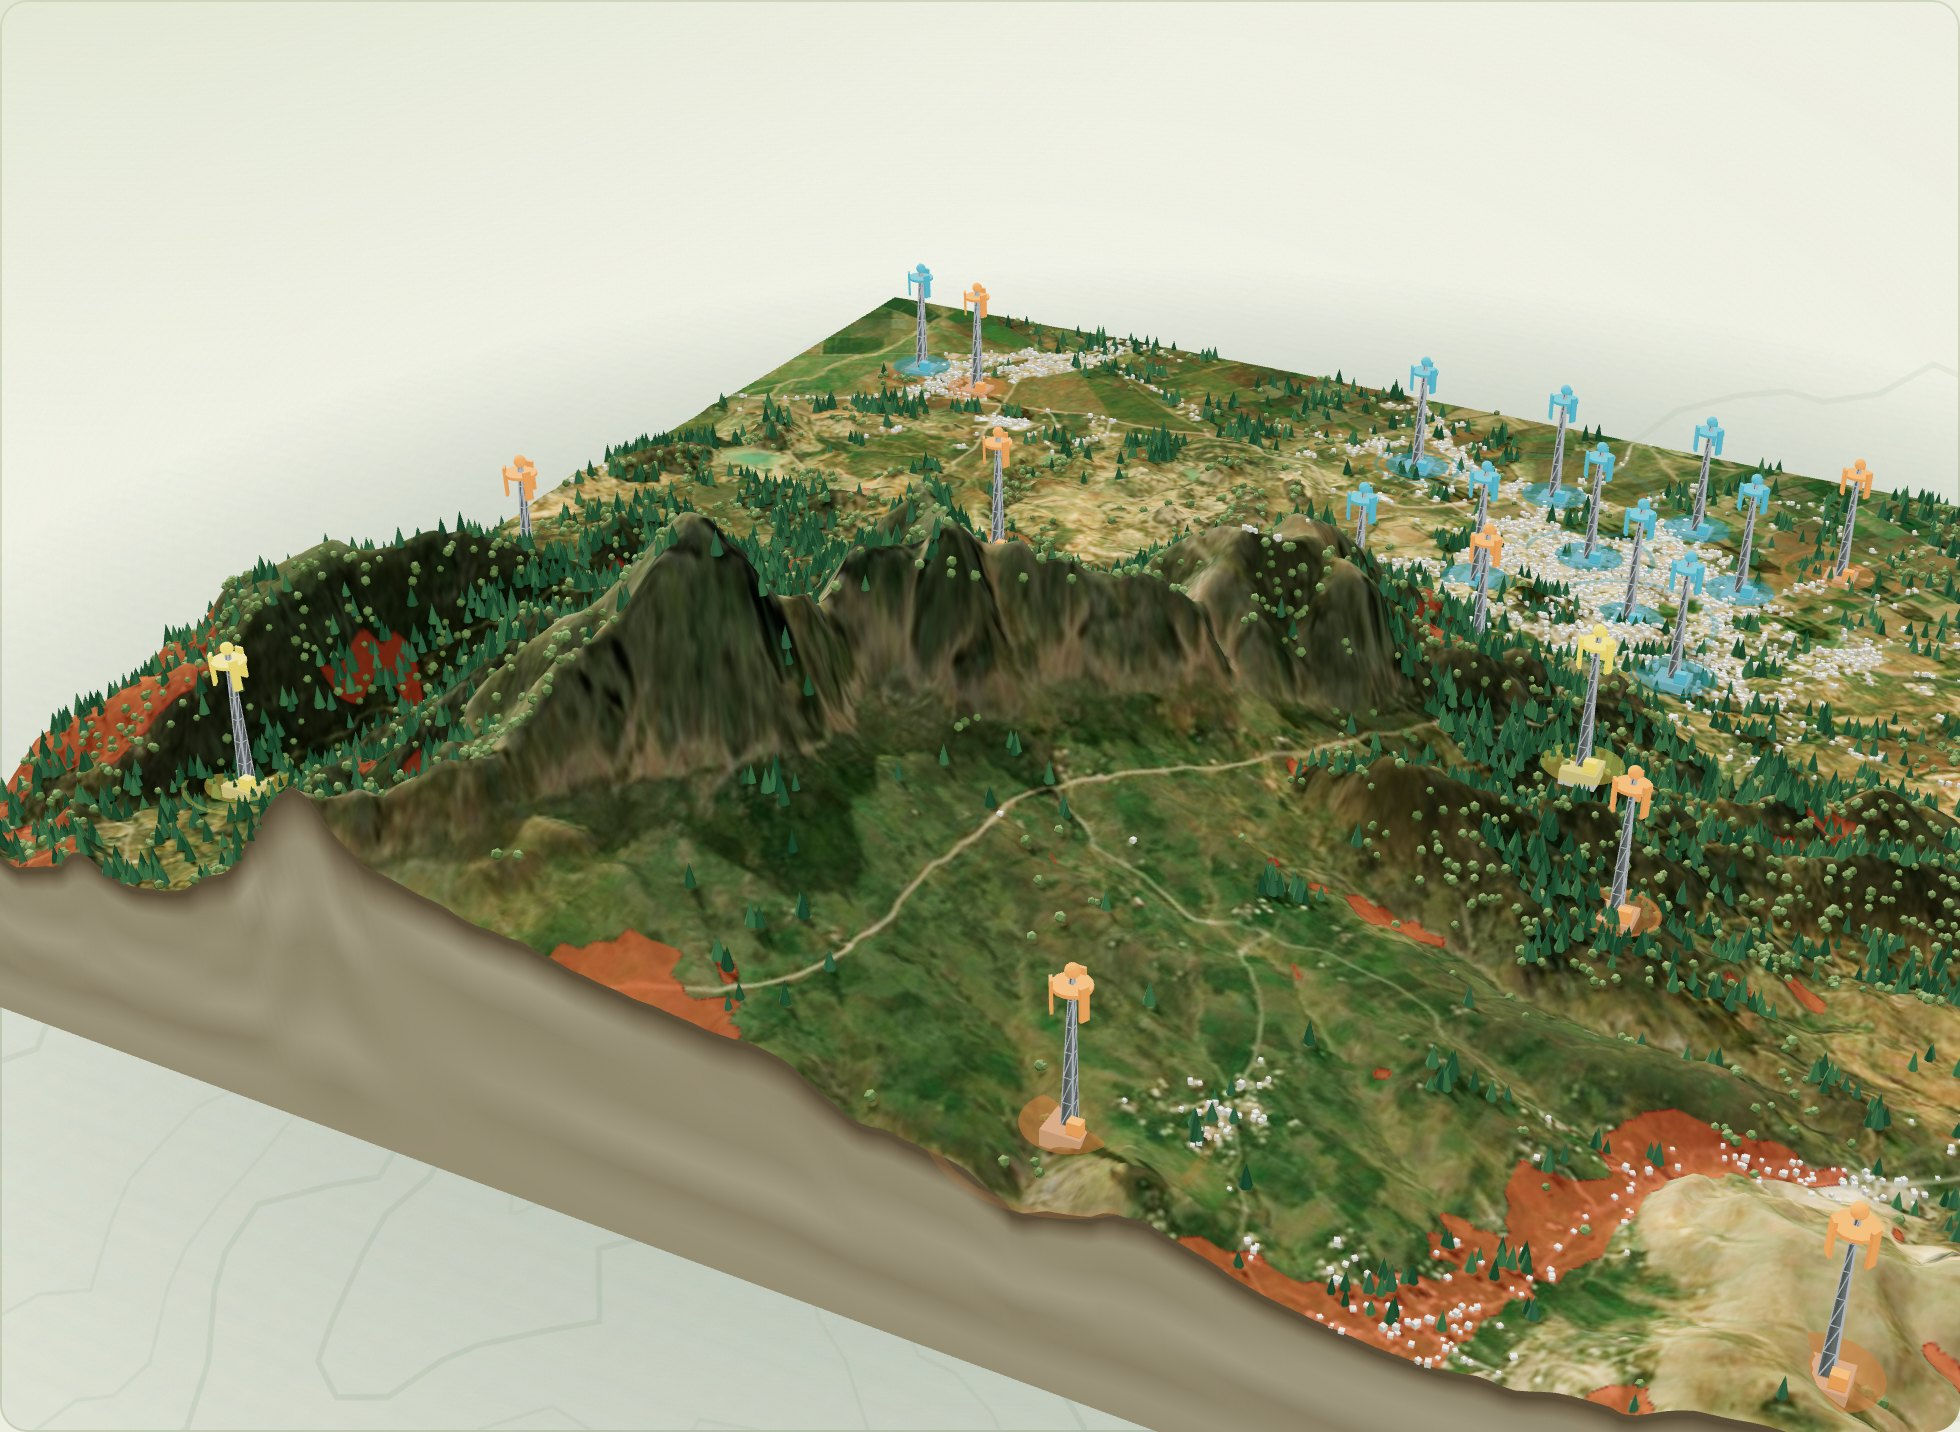
\includegraphics[width=0.62\textwidth]{ombre-final.jpg}
\caption{Le réseau final sur le relief.}
\label{fig-ombre-final}
\end{figure}

\begin{table}[H]
\centering
\caption{Réseau initial et réseau final.}
\label{tab-final}
\begin{tabularx}{\textwidth}{@{}Lccc@{}}
\toprule
\thead{Indicateur} & \thead{Initial} & \thead{Final} & \thead{Objectif} \\
\midrule
Couverture urbaine indoor & \SI{99,5}{\percent} & \textbf{\SI{99,7}{\percent}} & \SI{95}{\percent} \ok \\
Couverture rurale (surface / population) & \SI{83,4}{\percent} / \SI{95,4}{\percent} & \textbf{\SI{94,3}{\percent}} / \SI{97,9}{\percent} & \SI{95}{\percent} ($-0{,}7$ pt) \\
DL $\geq \SI{1}{\Mbps}$, ville (surface / population) & \SI{78,9}{\percent} / \SI{77,4}{\percent} & \SI{79,4}{\percent} / \SI{77,7}{\percent} & \SI{95}{\percent} \ko \\
DL $\geq \SI{1}{\Mbps}$, campagne (surface / population) & \SI{38,0}{\percent} / \SI{58,9}{\percent} & \SI{54,5}{\percent} / \SI{67,9}{\percent} & \\
UL $\geq \SI{128}{\kbps}$, ville & \SI{99,5}{\percent} & \SI{99,7}{\percent} & \SI{95}{\percent} \ok \\
UL $\geq \SI{128}{\kbps}$, campagne (surface / population) & \SI{55,8}{\percent} / \SI{83,0}{\percent} & \SI{73,9}{\percent} / \SI{89,6}{\percent} & \\
Surface couverte (toute la carte) & \SI{73,8}{\kilo\metre\squared} & \SI{86,8}{\kilo\metre\squared} & \\
Surface à 4 serveurs ou plus & \SI{2,39}{\kilo\metre\squared} & \SI{0,91}{\kilo\metre\squared} & \\
Nombre de sites & 20 & 21 & 21 (Étape 1) \\
\bottomrule
\end{tabularx}
\end{table}

Le \cref{tab-final} utilise les prédictions outdoor sauf mention, avec les charges simulées à \num{1000} utilisateurs. Pour les lignes DL et UL, la colonne \enquote{initial} est le réseau après l'action 1, recalculé avec les charges simulées (\cref{sec-charge}).

\subsection{Le Monte-Carlo final}

\begin{table}[H]
\centering
\caption{Monte-Carlo à \num{1000} utilisateurs, avant et après.}
\label{tab-mc-final}
\begin{tabular}{@{}lccc@{}}
\toprule
\thead{Indicateur} & \thead{Réseau initial} & \thead{Réseau final} & \thead{Évolution} \\
\midrule
Utilisateurs rejetés & 108,3 (\SI{10,8}{\percent}) & \textbf{76,8 (\SI{7,7}{\percent})} & $-\SI{29}{\percent}$ \\
\quad pas de couverture & 26,6 & 12,85 & divisé par 2 \\
\quad pas de service & 81,7 & 63,95 & $-\SI{22}{\percent}$ \\
\quad saturation & 0 & 0 & \\
Débit DL servi (cumulé) & \SI{257,3}{\Mbps} & \SI{281,1}{\Mbps} & $+\SI{9}{\percent}$ \\
Débit UL servi (cumulé) & \SI{68,3}{\Mbps} & \SI{70,5}{\Mbps} & $+\SI{3}{\percent}$ \\
\bottomrule
\end{tabular}
\end{table}

\begin{figure}[H]
\centering
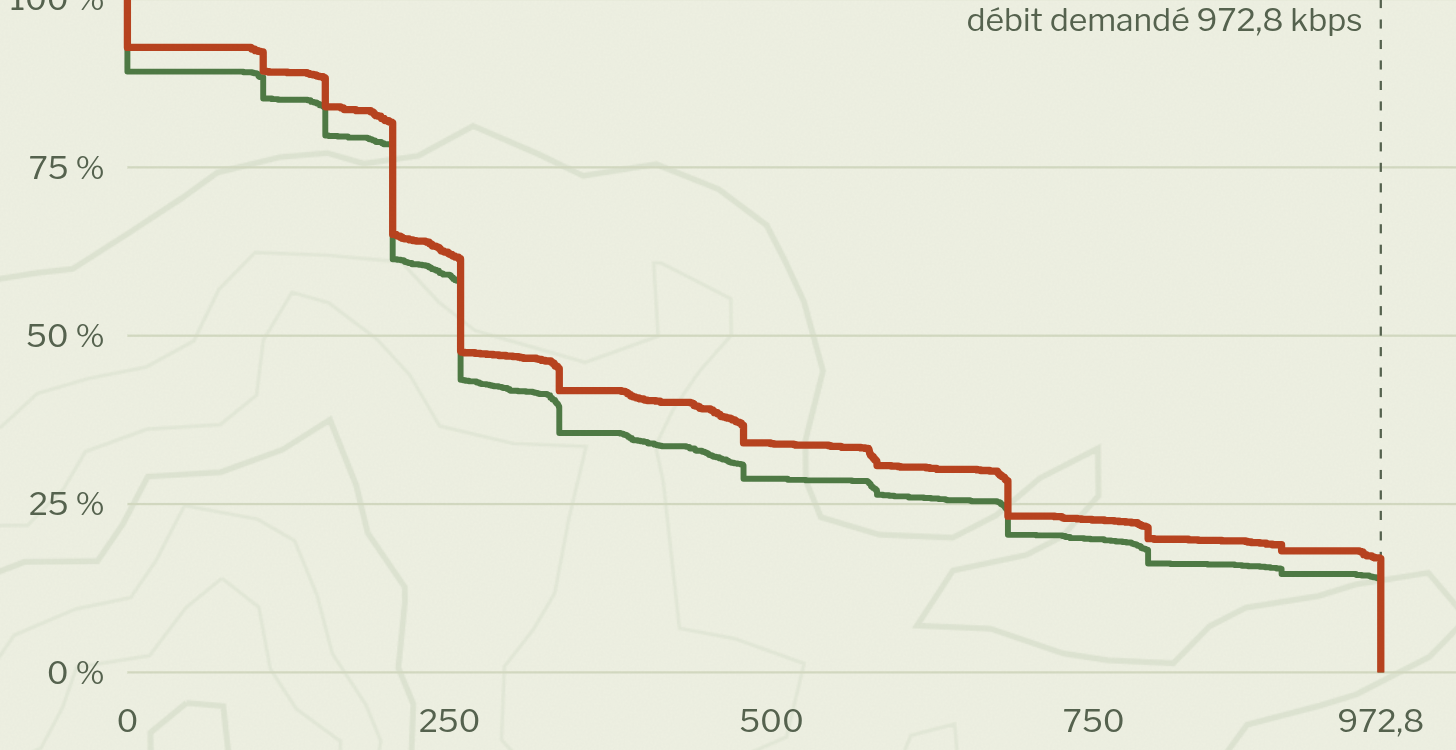
\includegraphics[width=0.66\textwidth]{dcfi-avant-apres.png}
\caption{DCFI DL à \num{1000} utilisateurs, avant et après.}
\label{fig-dcfi-final}
\end{figure}

Le \cref{tab-mc-final} donne la moyenne des 20 tirages, avec la même graine. Sur la \cref{fig-dcfi-final} (utilisateurs HSI, réseau initial en vert, final en terre cuite), toute la courbe monte d'environ 4 points : sur l'échantillon tracé, les rejets passent de \SI{10,5}{\percent} à \SI{6,7}{\percent} et la part des utilisateurs HSI servis au débit demandé de \SI{13,8}{\percent} à \SI{16,8}{\percent}. La médiane reste à \SI{259}{\kbps} : à \num{1000} utilisateurs, la limite est la capacité, que l'optimisation de la couverture ne règle pas (\cref{sec-p4}).

\subsection{Les mêmes utilisateurs, avant et après}

La graine fixée permet une comparaison directe : Atoll tire exactement les mêmes \num{1041} utilisateurs (mêmes positions, mêmes services) sur les deux réseaux. On peut donc suivre chaque utilisateur (\cref{fig-memes}). Sur la carte, un anneau or marque un utilisateur rejeté au départ et connecté sur le réseau final, un cercle creux terre cuite un utilisateur connecté au départ puis perdu, et une croix un utilisateur toujours rejeté.

\begin{figure}[H]
\centering
\begin{subfigure}[b]{0.5\textwidth}\centering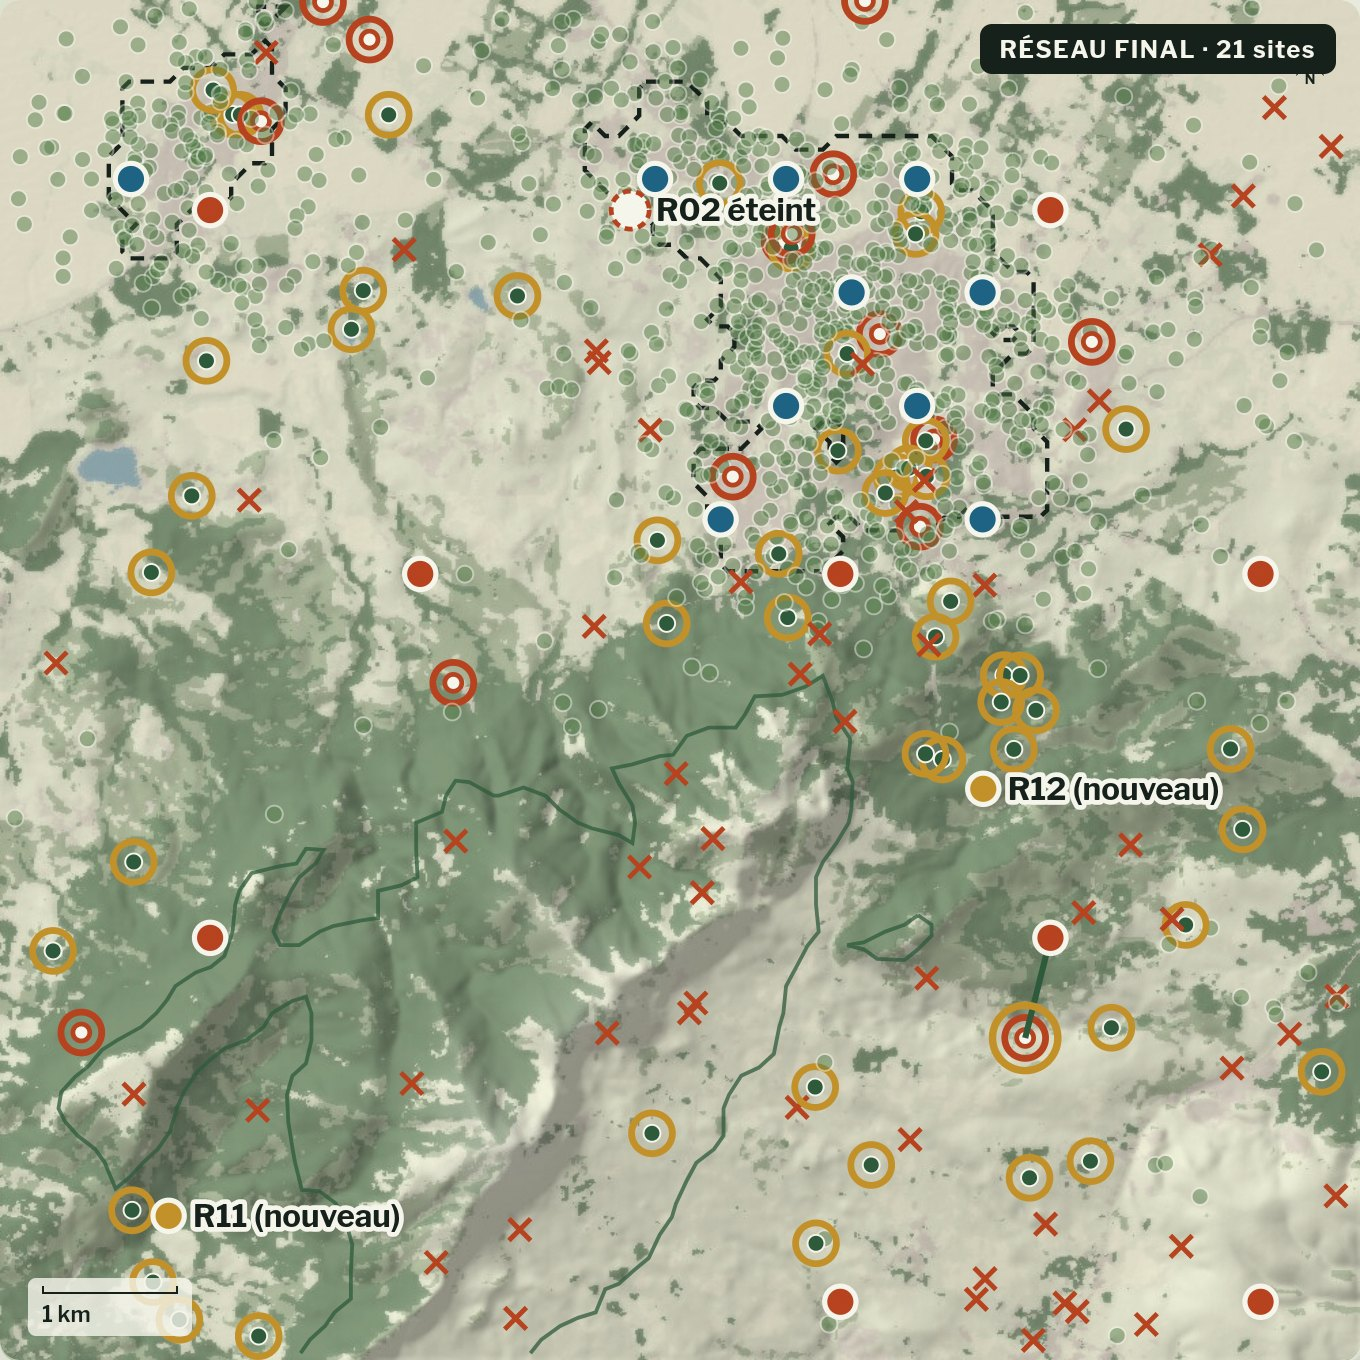
\includegraphics[width=\textwidth]{memes-utilisateurs.jpg}\caption{Réseau final.}\end{subfigure}\hfill
\begin{subfigure}[b]{0.47\textwidth}\centering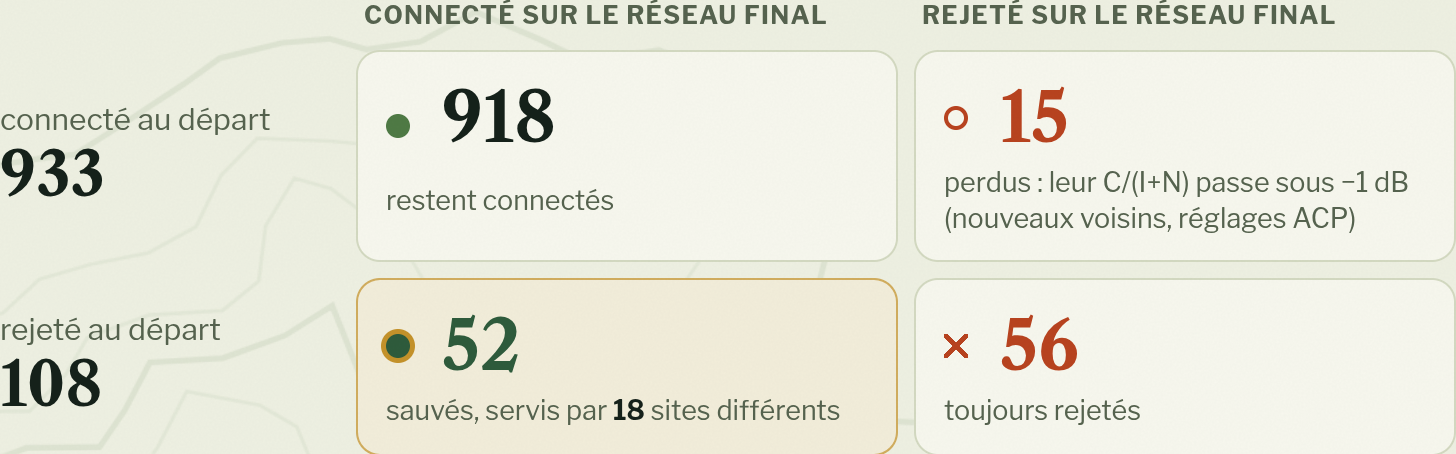
\includegraphics[width=\textwidth]{matrice-transitions.png}\caption{Transitions.}\end{subfigure}
\caption{Les mêmes \num{1041} utilisateurs sur les deux réseaux.}
\label{fig-memes}
\end{figure}

\begin{itemize}
  \item 52 utilisateurs rejetés sont sauvés. Ils sont servis par 18 sites différents, donc le gain vient de l'ensemble des actions (R11, R12 et les réglages de l'ACP). Par exemple, un utilisateur du coin sud-ouest sans couverture sur le réseau initial est servi par R11 avec un C/(I+N) de \SI{17,1}{\deci\bel}.
  \item 15 utilisateurs connectés sont perdus : leur C/(I+N) passe sous \SI{-1}{\deci\bel}, car les nouveaux sites et les réglages de l'ACP déplacent l'interférence.
  \item Au total, les rejetés passent de 108 à 71. Les 71 restants se trouvent dans la campagne isolée (46), sur le massif sans objectif (13) et en ville (12, dont 11 à l'intérieur des bâtiments), où la cause est l'interférence entre sites urbains.
\end{itemize}

\begin{retenir}
Cinq actions gardées (tilt urbain, R02 désactivé, R11, R12, ACP), trois rejetées après mesure (R07 déplacé, R07 réorienté, tilt à \ang{8}) et les relations de voisinage (ANR). La couverture rurale passe de \SI{83,4}{\percent} à \SI{94,3}{\percent}, la couverture urbaine reste au-dessus de \SI{99}{\percent}, avec 21 sites, et les rejets à \num{1000} utilisateurs passent de \SI{10,8}{\percent} à \SI{7,7}{\percent}.
\end{retenir}

\chapter{Étape 1 contre Étape 2 : discussion critique}
\label{ch-disc}

\section{Ce que la simulation confirme et ce qu'elle corrige}

\begin{table}[H]
\centering
\caption{Étape 1 et Étape 2 comparées.}
\label{tab-compare}
\begin{tabularx}{\textwidth}{@{}lLLl@{}}
\toprule
\thead{Grandeur} & \thead{Étape 1 (analytique)} & \thead{Étape 2 (Atoll)} & \thead{Verdict} \\
\midrule
Nombre de sites & 21 & 21, positions différentes ($-$R02, +R11, +R12) & confirmé \\
Couverture urbaine indoor & objectif \SI{95}{\percent} & \SI{99,7}{\percent} & atteint \\
Couverture rurale outdoor & objectif \SI{95}{\percent} & \SI{94,3}{\percent} de la surface, \SI{97,9}{\percent} de la population & $-0{,}7$ pt \\
Liaison limitante & montante, \SI{2}{\deci\bel} sous la descendante & DCFI UL insensible à la charge : limite de puissance du terminal & confirmé \\
Capacité & 5 sites suffiraient dans le centre & aucune saturation, même à \num{1000} utilisateurs & confirmé \\
Interférence ($K = 1$) & \SI{8,4}{\percent} de la cellule idéale sous \SI{-1}{\deci\bel} & \SI{21}{\percent} de la ville sous \SI{-1}{\deci\bel} avec la charge simulée & optimiste \\
Forme des cellules & cercles réguliers de \SI{0,64}{\kilo\metre} et \SI{2,06}{\kilo\metre} & ombres du relief au sud-ouest et au pied est & relief ignoré \\
\bottomrule
\end{tabularx}
\end{table}

La simulation confirme le nombre de sites, la liaison limitante et la conclusion sur la capacité : le calcul analytique a donné le bon ordre de grandeur. Quatre points changent.

\begin{itemize}
  \item Les positions. La formule de Hata ne voit pas le relief ; Atoll, avec la diffraction, calcule l'obstruction de la crête. Deux sites ont été ajoutés à l'intérieur des ombres du massif, et un site de la grille régulière s'est révélé inutile.
  \item L'interférence. L'hexagone idéal suppose des voisins réguliers sur un terrain plat. Le réseau réel a des sites perchés qui débordent loin dans la plaine, et Atoll applique la marge d'effet de masque aussi au C/(I+N). Le DL en ville reste ainsi à \SI{79}{\percent} de la surface au lieu de \SI{95}{\percent} ; sur ce point, notre calcul de l'Étape 1 était optimiste.
  \item La charge. Les prédictions par défaut supposent toutes les cellules chargées à \SI{100}{\percent}, alors que la charge simulée est de \SIrange{4}{31}{\percent}. Une même carte peut paraître très mauvaise ou acceptable selon cette hypothèse, qu'il faut donc toujours préciser.
  \item Le bord de cellule en UL. Dans l'Étape 1, le seuil de \SI{-120}{\dBm} et le débit UL de \SI{128}{\kbps} décrivent le même point. Dans Atoll, la surface couverte en outdoor (\SI{73,8}{\kilo\metre\squared}) dépasse la surface où l'UL atteint \SI{128}{\kbps} (\SI{48,6}{\kilo\metre\squared}). Les surcoûts et le taux d'erreur appliqués par Atoll pourraient exiger un troisième RB en bord de cellule, soit $10\log_{10}(3/2) \approx \SI{1,8}{\deci\bel}$ de moins par RB ; nous ne l'avons pas vérifié.
\end{itemize}

\section{Les notions du cours dans le projet}
\label{sec-cours}

Le \cref{tab-cours} reprend les notions du cours~\cite{afif2026cours} utilisées dans ce rapport, la façon dont nous les avons appliquées au LTE et le résultat obtenu.

\begin{table}[H]
\centering
\caption{Notions du cours et leur application.}
\label{tab-cours}
\small
\begin{tabularx}{\textwidth}{@{}>{\raggedright\arraybackslash}p{0.23\textwidth}>{\raggedright\arraybackslash}p{0.26\textwidth}L@{}}
\toprule
\thead{Notion du cours} & \thead{Formule ou règle} & \thead{Application et résultat} \\
\midrule
Objectif selon le contexte & urbain : capacité ; rural : couverture & trois zones ; la ville reste limitée par la couverture aujourd'hui (11 sites contre 5) \\
Bilan de liaison équilibré & bord de cellule atteint en UL et en DL & deux bilans ; UL limitante de \SI{2}{\deci\bel}, $R = \SI{0,64}{\kilo\metre}$ et \SI{2,06}{\kilo\metre} \\
Marge de fading & 10 à \SI{15}{\deci\bel} (FDMA) & \SI{0}{\deci\bel} en LTE, déjà dans les seuils des bearers ; sinon 3,7 fois plus de sites \\
Site tri-sectoriel & un site couvre trois cellules & 21 sites, 63 cellules ; $A_{\text{site}} = 1{,}95\,R^2$ \\
Taille du motif & $K = i^2 + ij + j^2$ & $K = 1$ avec $(i, j) = (1, 0)$ \\
Distance de réutilisation & $D = \sqrt{3K}\,R$, $q = D/R$ & $q = 1{,}73$ pour $K = 1$ \\
C/I au premier anneau & $C/I = (q - 1)^{\alpha} / 6$ & $\alpha = 3{,}52$ (pente de Hata) ; \SI{-12,6}{\deci\bel} au pire cas, \SI{8,4}{\percent} de la cellule sous \SI{-1}{\deci\bel} \\
Seuils de C/I & GSM \SI{9}{\deci\bel} : $K = 7$ ou 9 ; \SI{3}{\deci\bel} : $K = 3$ ou 4 & retrouvés par le calcul ; LTE à \SI{-1}{\deci\bel}, d'où $K = 1$ \\
Rendement d'un canal & $\eta$ = canaux de trafic / canaux totaux & GSM 0,75 ; LTE 0,71 en DL et 0,86 en UL \\
Capacité & $n\,\eta / (K \cdot B \cdot \pi R^2)$ & leviers utilisés : $K = 1$ et taille des cellules ; 5 sites suffisent aujourd'hui, 11 dans cinq ans \\
Boucle de planification & prédictions, ajustement, densification & huit actions mesurées, dont deux sites ajoutés \\
\bottomrule
\end{tabularx}
\end{table}

\section{Limites de l'étude}
\label{sec-limites}

\begin{itemize}
  \item Modèle non calibré. Aucune mesure terrain n'a permis d'ajuster le modèle Cost-Hata. L'incertitude de chaque pixel ($\sigma$ de 6 à \SI{8}{\deci\bel}) est bien plus grande que les 0,7 point qui manquent en campagne.
  \item Extrapolation du modèle. Le modèle de Hata est validé à partir de \SI{1}{\kilo\metre} ; le rayon urbain de \SI{0,64}{\kilo\metre} en est une légère extrapolation.
  \item Critère de qualité sévère. La marge d'effet de masque de \SI{86}{\percent} est appliquée aussi au C/(I+N) ; sans elle, la carte de qualité est nettement meilleure.
  \item Ordonnanceur d'Atoll. Même à 10 utilisateurs, \SI{46}{\percent} des utilisateurs HSI n'obtiennent pas \SI{1}{\Mbps} alors qu'ils sont seuls dans leur cellule avec un bon C/I. Nous n'avons pas trouvé la règle interne qui l'explique.
  \item Trafic modélisé. Un habitant vaut un utilisateur potentiel, et le mélange de services, de mobilités et de terminaux est une hypothèse.
  \item Antenne. Le diagramme d'antenne utilisé est défini à \SI{2100}{\mega\hertz} ; la bibliothèque d'Atoll contient un modèle à \SI{1800}{\mega\hertz} (\ang{65}, \SI{17}{\dBi}, tilt électrique de \ang{6}) qui serait plus juste.
  \item Objectifs non tous atteints. La campagne reste à \SI{94,3}{\percent} de la surface (\SI{97,9}{\percent} de la population) et le DL en ville à \SI{79}{\percent} de la surface.
\end{itemize}

\section{Perspectives}

Les réglages d'antenne ont atteint leur limite (action 7 rejetée). Les pistes suivantes portent sur l'architecture du réseau :
\begin{itemize}
  \item la coordination d'interférence entre cellules (ICIC) pour les bords de cellule urbains ;
  \item une couche à \SI{800}{\mega\hertz} sur les sites existants, qui apporterait de la portée en campagne et à l'intérieur des bâtiments, en complément du \SI{1800}{\mega\hertz} qui porte la capacité (\cref{sec-800-1800}) ;
  \item des petites cellules dans le centre quand le trafic aura doublé, au rythme actuel de +\SI{40}{\percent} tous les deux ans ;
  \item une campagne de mesures pour calibrer le modèle de propagation avant tout déploiement réel.
\end{itemize}

\chapter{Conclusion}
\label{ch-conclusion}

Ce projet a suivi la démarche d'un ingénieur planification radio sur une zone réelle de \SI{100}{\kilo\metre\squared} autour de Zaghouan.

Le dimensionnement analytique a fixé un réseau LTE en bande~3, avec une porteuse de \SI{20}{\mega\hertz} réutilisée dans toutes les cellules. Le bilan de liaison, limité par la liaison montante, donne un rayon de \SI{0,64}{\kilo\metre} en ville (indoor) et de \SI{2,06}{\kilo\metre} en campagne (outdoor). La couverture impose 21 sites tri-sectoriels ; la capacité n'en demanderait que 5 dans le centre aujourd'hui, mais en demanderait 11 dans cinq ans au rythme actuel de croissance du trafic.

Construit dans Atoll sur le relief, l'occupation du sol et la population réels, ce réseau couvre la ville mais laisse des trous derrière le massif. Les simulations Monte-Carlo à 10, 100 et \num{1000} utilisateurs montrent que les rejets viennent tous du signal et jamais de la capacité, que le débit descendant se dégrade avec la charge et que la liaison montante est limitée par la puissance du terminal.

Huit actions d'optimisation, mesurées une à une, ont porté la couverture rurale de \SI{83,4}{\percent} à \SI{94,3}{\percent} de la surface (\SI{97,9}{\percent} de la population) et maintenu la ville au-dessus de \SI{99}{\percent}. Trois actions ont été rejetées après mesure, et leurs échecs ont orienté les actions suivantes. Sur les mêmes utilisateurs simulés, les rejets ont baissé d'environ un tiers (de 108 à 71). Le réseau final compte 21 sites, le nombre prévu par le calcul.

Le calcul analytique a donné le bon nombre de sites, et la simulation sur le terrain réel leurs bons emplacements. Les formules du cours (bilan équilibré, motif et rapport C/I, rendement et capacité) ont guidé chaque choix de l'Étape 1, et leurs limites, comme le pire cas de C/I en réutilisation~1, ont été vérifiées dans Atoll. Les écarts restants (0,7 point en campagne, interférence en ville) sont dans l'incertitude d'un modèle non calibré, ou demandent des changements d'architecture (coordination d'interférence, seconde couche de fréquence, petites cellules) plutôt que de nouveaux réglages d'antenne.


\cleardoublepage
\phantomsection
\addcontentsline{toc}{chapter}{Bibliographie}
\renewcommand{\bibname}{Bibliographie}
\bibliography{references}

\appendix
\chapter{Coordonnées des sites}
\label{ann-sites}

Coordonnées en UTM 32N (EPSG:32632). Les 20 sites du plan nominal sont issus de l'Étape 1 ; l'altitude est lue sur notre MNT. Le réseau final retire R02 et ajoute R11 et R12. Tous les sites ont un mât de \SI{30}{\metre} et trois secteurs ; les azimuts nominaux (\ang{0}, \ang{120}, \ang{240}) et les tilts ont ensuite été ajustés par l'optimisation.

\begin{table}[H]
\centering
\caption{Sites du réseau.}
\label{tab-coords}
\small
\begin{tabular}{@{}lrrrl@{\hspace{2.5em}}lrrrl@{}}
\toprule
\thead{Site} & \thead{X (m)} & \thead{Y (m)} & \thead{Alt.} & \thead{Final} & \thead{Site} & \thead{X (m)} & \thead{Y (m)} & \thead{Alt.} & \thead{Final} \\
\midrule
U01 & 596\,963 & 4\,030\,684 & 161 & oui & R01 & 597\,545 & 4\,030\,455 & 173 & oui \\
U02 & 600\,817 & 4\,030\,684 & 155 & oui & R02 & 600\,634 & 4\,030\,455 & 162 & \textcolor{terre}{retiré} \\
U03 & 601\,780 & 4\,030\,684 & 146 & oui & R03 & 603\,724 & 4\,030\,455 & 128 & oui \\
U04 & 602\,744 & 4\,030\,684 & 131 & oui & R04 & 599\,090 & 4\,027\,780 & 270 & oui \\
U05 & 602\,262 & 4\,029\,850 & 152 & oui & R05 & 602\,179 & 4\,027\,780 & 283 & oui \\
U06 & 603\,225 & 4\,029\,850 & 145 & oui & R06 & 605\,269 & 4\,027\,780 & 164 & oui \\
U07 & 601\,780 & 4\,029\,015 & 195 & oui & R07 & 597\,545 & 4\,025\,104 & 503 & oui \\
U08 & 602\,744 & 4\,029\,015 & 178 & oui & R08 & 603\,724 & 4\,025\,104 & 393 & oui \\
U09 & 601\,299 & 4\,028\,181 & 241 & oui & R09 & 602\,179 & 4\,022\,428 & 419 & oui \\
U10 & 603\,225 & 4\,028\,181 & 235 & oui & R10 & 605\,269 & 4\,022\,428 & 401 & oui \\
 & & & & & R11 & 597\,240 & 4\,023\,060 & 391 & \textcolor{or!80!black}{ajouté} \\
 & & & & & R12 & 603\,230 & 4\,026\,200 & $\approx$ 430 & \textcolor{or!80!black}{ajouté} \\
\bottomrule
\end{tabular}
\end{table}

\chapter{Preuves et fichiers du projet}
\label{ann-preuves}

Le projet complet (calculs, cartes, projet Atoll, exports et présentation) est disponible en ligne :
\begin{itemize}
  \item dépôt : \url{https://github.com/Jozziiff/Atoll-Project-Zaghouan} ;
  \item présentation interactive : \url{https://jozziiff.github.io/Atoll-Project-Zaghouan/}.
\end{itemize}

\section*{Livrables Atoll (dossier \texttt{04-atoll/exports/})}

\begin{table}[H]
\centering
\caption{Correspondance entre les livrables du sujet (§\,4.2) et le rapport.}
\label{tab-livrables}
\footnotesize
\begin{tabularx}{\textwidth}{@{}p{0.17\textwidth}Lp{0.17\textwidth}p{0.2\textwidth}@{}}
\toprule
\thead{Livrable} & \thead{Contenu} & \thead{Dans ce rapport} & \thead{Fichiers} \\
\midrule
Niveau de signal & prédiction C/(I+N) et niveau de signal, histogramme, légende & \cref{sec-signal,sec-cinr} & \texttt{L-01*}, \texttt{L-02*} \\
Émetteur / recouvrement & prédiction par émetteur, histogramme de recouvrement, légende & \cref{sec-recouvrement} & \texttt{L-04*}, \texttt{L-05*} \\
Débit & débits DL et UL, légende, comparaison aux cibles & \cref{sec-debits,sec-charge} & \texttt{L-07*}, \texttt{L-08*} \\
Monte-Carlo & DCFI 10, 100 et \num{1000} utilisateurs & \cref{sec-dcfi} & \texttt{L-11*}, \texttt{dcfi*.md} \\
Optimisation & avant / après et justification de chaque action & \cref{ch-opt} & \texttt{trous\_*},\newline \texttt{couverture\_*} \\
\bottomrule
\end{tabularx}
\end{table}

\section*{Captures des réglages d'Atoll (dossier \texttt{04-atoll/captures/})}

Les captures sont nommées par séance de travail : \texttt{S01} import des cartes et modèles (coordonnées, MNT, occupation du sol, population, modèles de station, Cost-Hata, bearers, seuils) ; \texttt{S02} construction du réseau (valeurs par classe, table des sites et des émetteurs, correction de la population) ; \texttt{S03} prédictions (types disponibles, conditions, champs affichés, table des cellules, diagramme d'antenne) ; \texttt{S04} trafic et Monte-Carlo (carte de trafic, paramètres des simulations, statistiques, charges des cellules) ; \texttt{S05} optimisation (désactivation de R02, déplacement de R07, paramètres et résultats de l'ACP et de l'ANR).

\section*{Scripts}

\begin{table}[H]
\centering
\caption{Scripts du projet.}
\label{tab-scripts}
\small
\begin{tabularx}{\textwidth}{@{}lL@{}}
\toprule
\thead{Script} & \thead{Rôle} \\
\midrule
\texttt{02-dimensionnement/params.py} & tableau d'hypothèses sous forme de code, source unique des valeurs \\
\texttt{02-dimensionnement/calc.py} & Étape 1 complète : marges, bilans, rayons, sites, capacité, réutilisation, plan nominal, 800 contre \SI{1800}{\mega\hertz} \\
\texttt{03-cartes/scripts/make\_atoll\_maps.sh} & découpe, reprojection et mise au format Atoll des trois couches \\
\texttt{04-atoll/analyse\_couverture.py} & couverture par zone (surface, population) à partir des rasters exportés d'Atoll \\
\texttt{04-atoll/zones\_raster.py} & même mesure pour les cartes de C/(I+N) et de débit \\
\texttt{04-atoll/dcfi.py} & DCFI à partir des débits de chaque utilisateur exportés des simulations \\
\bottomrule
\end{tabularx}
\end{table}


\end{document}
